\documentclass[twocolumn, 10pt]{article}


% --- Page Layout --- %

\usepackage[utf8]{inputenc}
\usepackage{xcolor}
\usepackage{geometry}
\geometry{
	a4paper,
	left=20.0mm,
	right=20.0mm,
	top=20.0mm,
	bottom=22.0mm,
	columnsep=5.0mm,
	headsep=6.5mm,
	footskip=12.5mm
}
\usepackage[aux]{rerunfilecheck}
\usepackage{float}
\usepackage{dblfloatfix}


% --- Modern Font Setup --- %

\usepackage{fontspec}
\usepackage{unicode-math}
\setmainfont{TeX Gyre Termes}
\setmathfont{TeX Gyre Termes Math}


% --- Math Symbols --- %

\usepackage{amsmath}
\usepackage{mathtools}


% --- Units --- %

\usepackage[
	locale=US,
	per-mode = power,
	exponent-mode = input,
	print-unity-mantissa = false,
	range-units = single
]{siunitx}

\DeclareSIUnit{\year}{yr}
\DeclareSIUnit{\erg}{erg}
\DeclareSIUnit{\parsec}{pc}
\DeclareSIUnit{\angstrom}{\AA}
\DeclareSIUnit{\solarmass}{\ensuremath{M_\odot}}

\DeclareSIUnit{\dex}{dex}
\DeclareSIUnit{\rms}{rms}


% --- Aesthetic Improvements --- %

\usepackage{graphicx}
\usepackage{booktabs}
\usepackage{microtype}
\usepackage[autostyle]{csquotes}


% --- Draft Figures --- %

\usepackage[
	filename=false, 
	allfiguresdraft=draft
]{draftfigure}


% --- Float Improvements --- %

\usepackage{float}
\floatplacement{figure}{htbp}
\floatplacement{table}{htbp}

\usepackage[
	section,
	below,
]{placeins}


% --- Abstract Adjustments --- %

\usepackage{abstract}
\renewcommand{\abstracttextfont}{\small}
\setlength{\absleftindent}{0pt}
\setlength{\absrightindent}{0pt}
\setlength{\abstitleskip}{0.25\baselineskip}
\AfterEndEnvironment{abstract}{\vspace{1.5\baselineskip}}


% --- Section Styling --- %

\usepackage{titlesec}
\titleformat{\section}{\normalfont\large\bfseries}{\thesection}{1ex}{}
\titleformat{\subsection}{\normalfont\normalsize\bfseries}{\thesubsection}{1ex}{}


% --- Caption Styling --- %
\usepackage[
	labelfont=bf,
	font=small,
]{caption}
\usepackage{subcaption}

\captionsetup[figure]{width=0.9\columnwidth}
\captionsetup[figure*]{width=0.9\textwidth}

% --- Header & Footer --- %

\usepackage{fancyhdr}
\pagestyle{fancy}

\fancyhf{}
\renewcommand{\headrulewidth}{0pt}
\fancyfoot[C]{\itshape\thepage}

\fancypagestyle{plain}{
  \fancyhf{}
  \fancyfoot[C]{\itshape\thepage}
  \renewcommand{\headrulewidth}{0pt}
}


% --- Citation Setup --- %

\usepackage[american]{babel}

\usepackage[
	colorlinks=true, 
	linkcolor=black,      
	citecolor=black,      
	urlcolor=black
]{hyperref}

\usepackage[noabbrev, nameinlink]{cleveref}
\newcommand{\bcref}[1]{\textbf{\cref{#1}}}
\newcommand{\bCref}[1]{\textbf{\Cref{#1}}}

\usepackage[
	backend=biber,
	style=authoryear,
	giveninits=true,   
	maxnames=2,        
	minnames=1,
	uniquename=false,
	uniquelist=false
]{biblatex}

\DeclareNameAlias{author}{family-given} 
\DeclareDelimFormat{multinamedelim}{\addspace\&\addspace}
\DeclareDelimFormat{finalnamedelim}{\addspace\&\addspace}
\DefineBibliographyStrings{english}{andothers={et al.}} 

\DeclareFieldFormat{labeldate:extrayear}{}

\DeclareCiteCommand{\cite}[\mkbibparens]
	{\usebibmacro{prenote}}%
	{\usebibmacro{citeindex}%
	 \printtext[bibhyperref]{%
	 	\printnames{labelname}%
	 	\setunit{\addspace}%
	 	\printfield{labelyear}%
	 	\printfield{extrayear}%
	 }%
	}%
	{\multicitedelim}%
	{\usebibmacro{postnote}}%

\DeclareDelimFormat{multicitedelim}{\addcomma\addspace}

\DeclareFieldFormat[article,periodical]{journaltitle}{\textit{#1}}

\DeclareFieldFormat[article]{title}{}
\DeclareFieldFormat[book]{title}{}

\AtEveryBibitem{%
	\clearfield{volume}%
	\clearfield{number}%
	\clearfield{pages}%
	\clearfield{note}%
	\clearfield{location}%
	\clearfield{address}%
}

\renewcommand{\finentrypunct}{}

\DeclareBibliographyDriver{article}{%
	\usebibmacro{bibindex}%
	\usebibmacro{begentry}%
	\iffieldundef{doi}
		{\iffieldundef{url}
			{\printnames{author}\setunit{\addspace}%
			 \usebibmacro{journal}\setunit{\addspace}%
			 \printtext{\mkbibparens{\printfield{labelyear}\printfield{extrayear}}}}%
			{\href{\thefield{url}}{%
				\printnames{author}\setunit{\addspace}%
				\usebibmacro{journal}\setunit{\addspace}%
				\printtext{\mkbibparens{\printfield{labelyear}\printfield{extrayear}}}}}}
		{\href{https://doi.org/\thefield{doi}}{%
			\printnames{author}\setunit{\addspace}%
			\usebibmacro{journal}\setunit{\addspace}%
			\printtext{\mkbibparens{\printfield{labelyear}\printfield{extrayear}}}}}%
	\usebibmacro{finentry}%
}

\addbibresource{source.bib}


% --- Paragraph Skip --- %

\usepackage{parskip}
\setlength{\parindent}{0pt}
\setlength{\parskip}{0.4\baselineskip plus 2pt minus 2pt}


% --- Linted Code --- %

\usepackage{varwidth}
\usepackage{listings}
\usepackage{accsupp}

\newcommand{\noncopynumber}[1]{%
     \BeginAccSupp{ActualText={}}#1\EndAccSupp{}%
}

\definecolor{firebrick}{RGB}{178, 34, 34}     
\definecolor{goldenrod}{RGB}{218, 165, 32}    
\definecolor{olivedrab}{RGB}{107, 142, 35}    
\definecolor{steelblue}{RGB}{70, 130, 180}    
\definecolor{rebeccapurple}{RGB}{102, 51, 153}

\definecolor{lightergray}{RGB}{250, 250, 250} 
\definecolor{lightishgray}{RGB}{180, 180, 180}

\lstset{
	language=SQL,                          
	backgroundcolor=\color{lightergray},   
	basicstyle=\ttfamily\footnotesize\color{black},
	identifierstyle=\color{black},
	keywordstyle=\color{steelblue}\bfseries, 
	stringstyle=\color{goldenrod},        
	morekeywords=[2]{TOP, APPLY},
	keywordstyle=[2]{\color{firebrick}\bfseries},
	numberstyle=\tiny\color{lightishgray}\noncopynumber, 
	numbers=left,                          
	numbersep=8pt,                         
	breaklines=true,                       
	breakatwhitespace=false,               
	showstringspaces=false,                
	keepspaces=true,
	frame=single,                          
	rulecolor=\color{black},
	tabsize=4,                             
	keywordsprefix=,
	literate=*
		{=}{{{\color{rebeccapurple}=}}}1
		{!=}{{{\color{rebeccapurple}!=}}}2
		{<}{{{\color{rebeccapurple}<}}}1
		{>}{{{\color{rebeccapurple}>}}}1
		{+}{{{\color{rebeccapurple}+}}}1
		{-}{{{\color{rebeccapurple}-}}}1
		{*}{{{\color{rebeccapurple}*}}}1
		{:}{{{\color{rebeccapurple}:}}}1
		{10000}{{{\color{olivedrab}10000}}}5
		{\ 1\ }{{{\ \color{olivedrab}1\ }}}3
		{\ 3}{{{\ \color{olivedrab}3}}}2
		{0\.35}{{{\color{olivedrab}0.35}}}4
		{\ 0\.0}{{{\ \color{olivedrab}0.0}}}4
		{5\.0}{{{\color{olivedrab}5.0}}}3
		{2\.355}{{{\color{olivedrab}2.355}}}5
		{\ 500}{{{\ \color{olivedrab}500}}}4
}


% --- Dummy Text --- %

\usepackage{lipsum}


% --- Writing Lengths --- %

\AtEndDocument{
	\directlua{
		local factor = 65536 * 72.27
		
		local tw = math.floor((tex.getdimen("textwidth") / factor) * 100 + 0.5) / 100
		local cw = math.floor((tex.getdimen("columnwidth") / factor) * 100 + 0.5) / 100
		local cs = math.floor((tex.getdimen("columnsep") / factor) * 100 + 0.5) / 100
		local lw = math.floor((tex.getdimen("linewidth") / factor) * 100 + 0.5) / 100
		
		texio.write_nl("===================================================")
		texio.write_nl("CURRENT LAYOUT:")
		texio.write_nl("Textwidth:  " .. tw .. " in")
		texio.write_nl("Columnwidth: " .. cw .. " in")
		texio.write_nl("Columnsep:   " .. cs .. " in")
		texio.write_nl("Linewidth:   " .. lw .. " in")
		texio.write_nl("===================================================")
		io.flush()
	}
}



% --- Title --- %

\title{\textbf{Numerical Simulations of AGN Accretion Disks in PLUTO}}%


% --- Author --- %

\author{Fritz Ali Agildere%
		\vspace{-0.5ex}\\\small\href{mailto:fritz.agildere@udo.edu}{fritz.agildere@udo.edu}%
		\\\small\textit{Nicolaus Copernicus Astronomical Center, Polish Academy of Sciences, Warsaw}}%


% --- Compilation Date --- %

\date{\small \today}


% --- Header & Footer --- %

\fancyhead[C]{\textit{Numerical Simulations of AGN Accretion Disks in PLUTO}}
\fancyfoot[L]{Summer Student Program 2026}
\fancyfoot[R]{CAMK PAN \& EMJM MASS}

\fancypagestyle{plain}{
	\fancyhead[C]{}
	\fancyfoot[L]{Summer Student Program 2026}
	\fancyfoot[R]{CAMK PAN \& EMJM MASS}
}


% --- Custom Macros --- %

\newcommand{\dash}{\rule[0.49ex]{0.35em}{0.06em}}
\newcommand{\xray}{X\hspace{0.04em}\dash\hspace{0.11em}ray\space}
\newcommand{\xrays}{X\hspace{0.04em}\dash\hspace{0.11em}rays\space}


% --- Metadata --- %

\hypersetup{
	pdfauthor={Fritz Ali Agildere},
	pdftitle={Course Report – Fritz Agildere}
}


% --- Float Setup --- %

\renewcommand{\topfraction}{0.9}   
\renewcommand{\bottomfraction}{0.8}
\renewcommand{\textfraction}{0.1}  
\renewcommand{\floatpagefraction}{0.7}




% --- Line Breaking --- %

\raggedbottom
\hyphenpenalty=10000
\exhyphenpenalty=10000
\emergencystretch=2em


% --- Begin Document --- %

\begin{document}

	\twocolumn[{
		\maketitle
		\begin{abstract}
			We present two dimensional radiation hydrodynamic simulations of a thin viscous accretion disk around a nonrotating
			supermassive black hole with a mass of \qty{1e8}{\solarmass} in the PLUTO code. Starting from an existing star disk setup with
			viscosity and resistivity, we replace the central star with an absorbing inner boundary and a Paczyński–Wiita potential, and
			add the nonrelativistic two moment radiation module with Kramers, Thomson and an effective Compton opacity. Once radiation is
			enabled, the advected passive tracer that restricted viscosity, resistivity and opacities to the disk no longer follows the
			disk material. We therefore develop a replacement called DiskFraction, which classifies each cell from its density relative to
			adaptive radial reference profiles and from its rotation. We validate the classifier against the tracer in hydrodynamic,
			magnetohydrodynamic and resistive runs without radiation, and then use it in two radiation runs at different resolutions.
			Both reach statistically steady states with accretion rates of about \num{0.07} to \num{0.09} times the Eddington rate and
			a radiative efficiency close to \num{0.048} in both runs. They carry quasiperiodic density waves that travel outward with a period of
			about \num{350} gravitational times, and a weak inflow stream at intermediate altitudes. We discuss which of these features
			may be artifacts of the fixed sound speed in the viscosity prescription, of the boundaries and of the physics still missing
			from the setup.
		\end{abstract}
	}]

	\section{Introduction}

	Active Galactic Nuclei (AGN) are powered by accretion onto Super Massive Black Holes (SMBH). In the standard picture, the gas
	forms a geometrically thin disk in which an effective viscosity transports angular momentum outward and converts gravitational
	energy into heat that is radiated away locally \cite{shak1973}. For accretion rates around a tenth of the Eddington rate, the inner
	parts of such disks are dominated by radiation pressure, and in this regime the standard disk with a viscous stress proportional
	to the total pressure is thermally and viscously unstable \cite{ligh1974, shak1976}. Whether real disks follow this prediction,
	and what happens to them if they do, is a question that requires following the coupled evolution of gas and radiation in time,
	which is what numerical simulations can do.

	In this work, we build such a setup in the PLUTO code \cite{mign2007}. We start from an existing setup for the interaction of a
	star with its accretion disk \cite{ceme2019}, adapt it to a black hole and then enable radiation. Along the way, we find that the
	passive tracer used to separate disk and corona, and with it the physics restricted to the disk, stops working once radiation is
	enabled. Most of our effort therefore went into a replacement for this tracer, the DiskFraction classifier, which we describe and
	validate in \Cref{sec:classifier}. With this classifier, we then run the radiation setup at two resolutions until both reach a
	steady state, and present first results in \Cref{sec:results}. The limitations of the setup are discussed in
	\Cref{sec:discussion}. Equations of secondary importance, the analysis methods, supplementary figures and the link to all source
	files are included in the \hyperref[sec:appendix]{appendix}.

	\section{Numerical Setup}
	\label{sec:setup}

	All simulations use version 4.4 of PLUTO \cite{mign2007} on a two dimensional grid in spherical coordinates, with radius $r$ and
	polar angle $\theta$ as well as axisymmetry and equatorial symmetry, so that only one hemisphere is simulated. We also use the
	cylindrical radius $R = r \sin\theta$ and the height $z = r \cos\theta$ above the midplane in what follows.

	\subsection{Base Model}

	The starting point is a star disk setup from a numerical atlas of such systems \cite{ceme2019}, which solves the equations of viscous and
	resistive magnetohydrodynamics for a thin disk around a rotating star with a magnetic field. The initial disk follows an
	analytic solution for a thin viscous disk \cite{kluz2000} with aspect ratio $\epsilon = H/R$ and is embedded in a corona in
	hydrostatic equilibrium. Viscosity and resistivity follow an alpha prescription and are restricted to the disk by a passive
	tracer, which is advected with the flow and initially equals one in the disk and zero in the corona. To keep the disk thin
	without radiative cooling, the setup also includes an artificial cooling term, which S. Kundu and M. Čemeljić use in their setup.
	It removes a multiple of the local viscous and Ohmic heating from the disk gas, again weighted by the tracer, wherever this
	removal stays below ten percent of the thermal energy of the cell. Its exact form is given in \Cref{app:equations}.

	\subsection{Black Hole Adaptation}

	Our first tests ran on the stellar setups of the atlas. For a black hole, we replace the stellar surface at the inner radial
	boundary with an absorbing diode condition, which copies the state of the first active cell but lets gas and radiation only
	flow inward. The gravity of the star is replaced with the pseudo Newtonian potential \cite{pacz1980}
	\begin{equation}
		\Phi = -\frac{G M}{r - r_s}
	\end{equation}
	where $r_s = 2 G M / c^2$ is the Schwarzschild radius. Within Newtonian dynamics, this potential reproduces the innermost stable
	circular orbit of a nonrotating black hole at six gravitational radii, and with it the efficiency $\eta = 1/16$ of a disk that
	ends there. Lengths are measured in gravitational radii $r_g = G M / c^2$ and times in gravitational times $t_g = r_g / c$ with
	velocities in units of $c$ accordingly. Without radiation, the equations solved here contain no other scale, so all results
	of the non radiative runs hold for any black hole mass.

	The domain extends from $r = 2.1$ to $r = 30$ in gravitational radii on a logarithmic radial grid and from the pole to the
	midplane on a uniform polar grid. The initial disk has $\epsilon = 0.1$ and an inner edge at $R = 6$ in these units, while
	the corona has the density profile $\rho_c \propto r^{-3/2}$ with a normalization of \num{0.01} in code units. At the
	outer boundary, the analytic disk is reinjected in a narrow wedge around the midplane, while inflow of coronal gas is
	blocked at higher latitudes. All tests of the tracer and the classifier in \Cref{sec:classifier} were performed in this
	black hole setup, that is for a nonrotating black hole under Newtonian dynamics with the pseudo potential, with and without
	magnetic fields and resistivity.

	\subsection{Radiation and Physical Units}

	For radiation, we use the nonrelativistic version of the two moment radiation module of PLUTO \cite{melo2019, melo2021} with
	the full speed of light. Radiation introduces physical scales through the opacities and the radiation constant, so the units
	have to be fixed. We choose a black hole mass of \qty{1e8}{\solarmass} for all radiation runs, which gives $r_g \approx \qty{1.48e13}{\centi\meter}$
	and $t_g \approx \qty{493}{\second}$ as units. The density unit $\rho_0 = \qty{5.8e-10}{\gram\per\centi\meter\cubed}$ is
	chosen together with the viscosity parameter $\alpha = 0.5$ so that viscous heating and radiative cooling of the initial
	disk roughly balance, which corresponds to accretion at around a tenth of the Eddington rate. A twenty times higher density
	unit with $\alpha = 1$ gave a heating excess equivalent to strongly super Eddington accretion, and the disk was disrupted
	within a few hundred gravitational times. In the radiation runs, the artificial cooling is removed, since the radiation now
	carries the heat away.

	For the opacities, we assume a hydrogen mass fraction $X = 0.7$ and a metallicity $Z = 0.02$ and include Kramers free free and
	bound free absorption \cite{kram1923} as well as Thomson scattering with $\kappa_\mathrm{es} = 0.2 \left(1 + X\right)$ in
	units of square centimeters per gram. PLUTO treats scattering as coherent, so in this form electron scattering never
	exchanges energy between gas and radiation. In AGN disks, however, it is Compton scattering that keeps the gas close to the
	radiation temperature, and without it viscous heating drove the gas in the inner disk to between \num{1e10} and
	\qty{1e11}{\kelvin} in our tests, until overpressured bubbles broke the disk apart. We therefore add an effective absorption
	opacity
	\begin{equation}
		\kappa_C = \kappa_\mathrm{es} \frac{4 k_B T_r^4}{m_e c^2 \left(T_g + T_r\right) \left(T_g^2 + T_r^2\right)}
		\label{eq:compton}
	\end{equation}
	with gas temperature $T_g$ and radiation temperature $T_r$ as inputs. With this opacity, the absorption term
	$\rho \kappa_C c \left(a_R T_g^4 - E_r\right)$ reproduces exactly the nonrelativistic Compton exchange rate
	\begin{equation}
		\Lambda_C = 4 \rho \kappa_\mathrm{es} c E_r \frac{k_B \left(T_g - T_r\right)}{m_e c^2}
	\end{equation}
	since the factor $T_g - T_r$ cancels analytically against $T_g^4 - T_r^4$ in the absorption form. This rate is the usual
	approximation for Compton cooling and heating in radiation hydrodynamics, and a term of this form is used for example in
	radiation magnetohydrodynamic simulations of accretion disks \cite{jian2019}. The Compton part is moved from scattering to absorption, so
	the total extinction stays that of Thomson scattering and only the energy exchange changes. Several safeguards complete the
	opacity model and are listed in \Cref{app:equations}. They hold the Compton rate fixed above a gas temperature of
	\qty{1e9}{\kelvin} and switch the energy exchange off in the corona and in gas that moves faster than about nine tenths of
	the speed of light. A floor of \qty{1e4}{\kelvin} for the gas temperature prevents surface layers from cooling far below the
	range in which the opacity model is valid.

	\section{Disk Classifier}
	\label{sec:classifier}

	In the base model, the passive tracer decides where viscosity, resistivity, artificial cooling and later the opacities act.
	Once radiation is enabled, this tracer stops following the disk material in our runs. It stays at its initial distribution,
	while the disk itself evolves, as the left column of \Cref{fig:valid_rad} shows. We did not isolate the cause of this in the
	code. But even without radiation, an advected scalar is smeared out by numerical diffusion where it has steep gradients, which
	on an Eulerian grid is mainly the disk surface. We therefore replace the tracer with a classifier that derives the disk
	membership of each cell from its current state alone.

	\subsection{Construction}

	DiskFraction assigns each cell a value $f$ between zero for corona and one for disk from two criteria. The first compares the
	density $\rho$ of the cell with a corona reference density $\rho_c(r)$ and a disk reference density $\rho_d(r)$ at its radius,
	which are stored in \num{90} logarithmic radial bins and interpolated linearly in logarithmic radius and density. With the
	relative position of the cell between these references
	\begin{equation}
		s = \frac{\log \rho - \log \rho_c}{\max\left(\log \rho_d - \log \rho_c, \, 0.5\right)}
	\end{equation}
	and the logistic function $\sigma(x) = 1 / \left(1 + e^{-x}\right)$ the classifier reads
	\begin{equation}
		f = \sigma\left(\frac{s - 1/6}{0.3}\right) \sigma\left(\frac{\lvert v_\phi \rvert \sqrt{R} - 0.5}{0.1}\right)
		\label{eq:diskfrac}
	\end{equation}
	where the second factor compares the rotation velocity $v_\phi$ with the Newtonian Keplerian velocity $R^{-1/2}$ in code units,
	so that only dense and rotating gas counts as disk. The midpoint of the density criterion lies one sixth of the way from the
	corona to the disk reference in logarithmic density. At the start of a run, before any profile has been updated, the classifier $f$ equals
	exactly the initial tracer, since both are evaluated from the same condition that sets up the disk.

	By default, the references are built from the classification itself. After every time step, the corona reference of a bin
	becomes the mean density weighted with $1 - f$ and the disk reference the mean density weighted with $f$ over all cells in the
	bin. A disk estimate only counts if its weighted volume exceeds one thousandth of the bin volume, and bins that never had one
	copy the nearest valid bin. Both profiles are smoothed in time by an exponential moving average, which gives each new estimate
	the weight
	\begin{equation}
		w = 1 - \exp\left(-\frac{\Delta t}{\tau}\right)
		\label{eq:ema}
	\end{equation}
	with the time $\Delta t$ between two updates and the time constant $\tau = 6 \, t_g$ as parameters. The state of the
	classifier is written with every output, so that restarts continue with exactly the same classification.

	\subsection{Versions and Guards}

	The first version of the classifier gave each update the fixed weight \num{0.05} instead. Updated after every step, the profiles
	then had a memory of about twenty steps, which depends on resolution and corresponds to about \num{0.12} and \num{0.17}
	gravitational times at the two resolutions used below. In a run with this version at the higher resolution, the density
	criterion inverted after the disk had been disrupted. In the bins at radii between about \num{2.4} and \num{3.4} the
	disk reference stayed about one dex below the corona reference until the end of the run. Since the references were built
	from the classification, this inversion sustained itself, as dense gas classified as corona raised the corona reference and
	thin gas classified as disk lowered the disk reference. The rotation criterion could not compensate, because gas plunging
	inside the innermost stable orbit keeps its specific angular momentum of about \num{3.7} and therefore rotates two to
	three times faster than the Newtonian Keplerian velocity there. The result was a region close to the black hole classified
	as disk up to about \ang{45} above the midplane, while the dense plunging stream inside it lost its viscosity and its coupling
	to the radiation.

	The current version therefore adds three guards. The logarithmic span between the references used in the classification is
	at least \num{0.5} dex, as already included in the denominator of $s$ above, so an inverted span can no longer flip the
	density criterion. After every update, bins with a smaller span copy both references from the nearest bin with a sufficient
	span, searching outward first, or have their disk reference raised to the minimum span if no such bin exists. Finally, the
	smoothing uses the time constant of \Cref{eq:ema} instead of a fixed weight, so that the memory of the profiles is the same
	at every resolution and update cadence. Slight artifacts at the inner boundary still appear in this version, but the guards
	let the classifier repair itself instead of locking an error in place.

	As an option, the references can also be built without reference to the classification. The disk reference is then the
	maximum density of each bin and the corona reference the geometric mean density of the cells above $z / R = 0.5$ in that bin.
	This mode cannot feed back on itself, but it has been tested much less than the default and is not used for the results
	presented here.

	\subsection{Validation}

	To test the classifier, we ran the black hole setup without radiation as hydrodynamic, magnetohydrodynamic and resistive
	magnetohydrodynamic simulations with \num{90} by \num{45} cells up to $t = 1000$ in gravitational times. Each case was run
	twice. In the tracer driven run, the tracer decides where viscosity, resistivity and the artificial cooling act. In the
	classifier driven run, DiskFraction takes this role, while the tracer is still advected passively and can be compared.
	\Cref{fig:valid_rho} compares the density of both hydrodynamic runs, and \Cref{fig:valid_class} the tracer and the
	classifier within the classifier driven run. The disk body is identified by both in the same way, and the differences
	concentrate in the surface layer, where the tracer is smeared out. \Cref{fig:valid_agreement} quantifies the agreement over
	time for all three cases, and the corresponding maps of the magnetohydrodynamic cases are included in
	\Cref{app:figures}. With radiation, on the other hand, the tracer remains at its initial wedge while the classifier follows
	the disk, as shown in \Cref{fig:valid_rad}.

	\begin{figure*}[t]
		\centering
		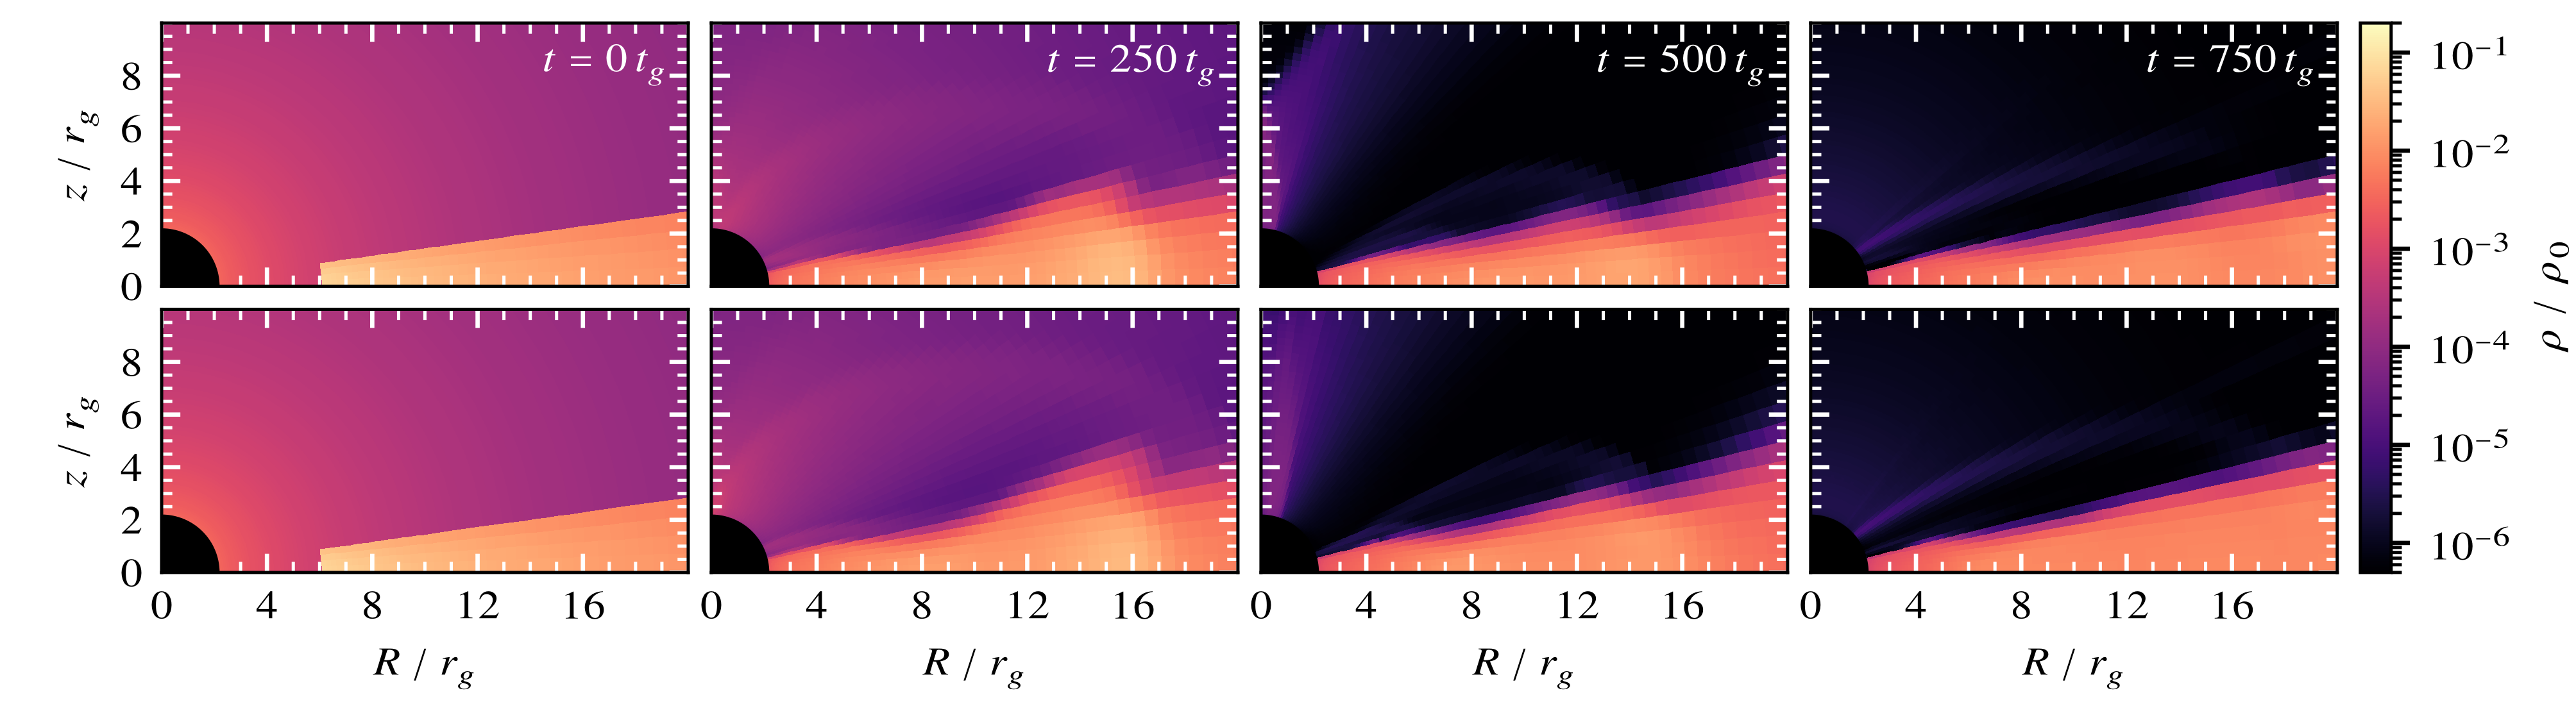
\includegraphics[width=\textwidth, draft=false]{plots/valid_hd_rho_text.png}
		\caption{Density in the hydrodynamic black hole setup without radiation. \textit{Top:} Run in which the passive tracer
				 restricts viscosity and artificial cooling to the disk. \textit{Bottom:} Run in which DiskFraction takes this role.}
		\label{fig:valid_rho}
	\end{figure*}

	\begin{figure*}[t]
		\centering
		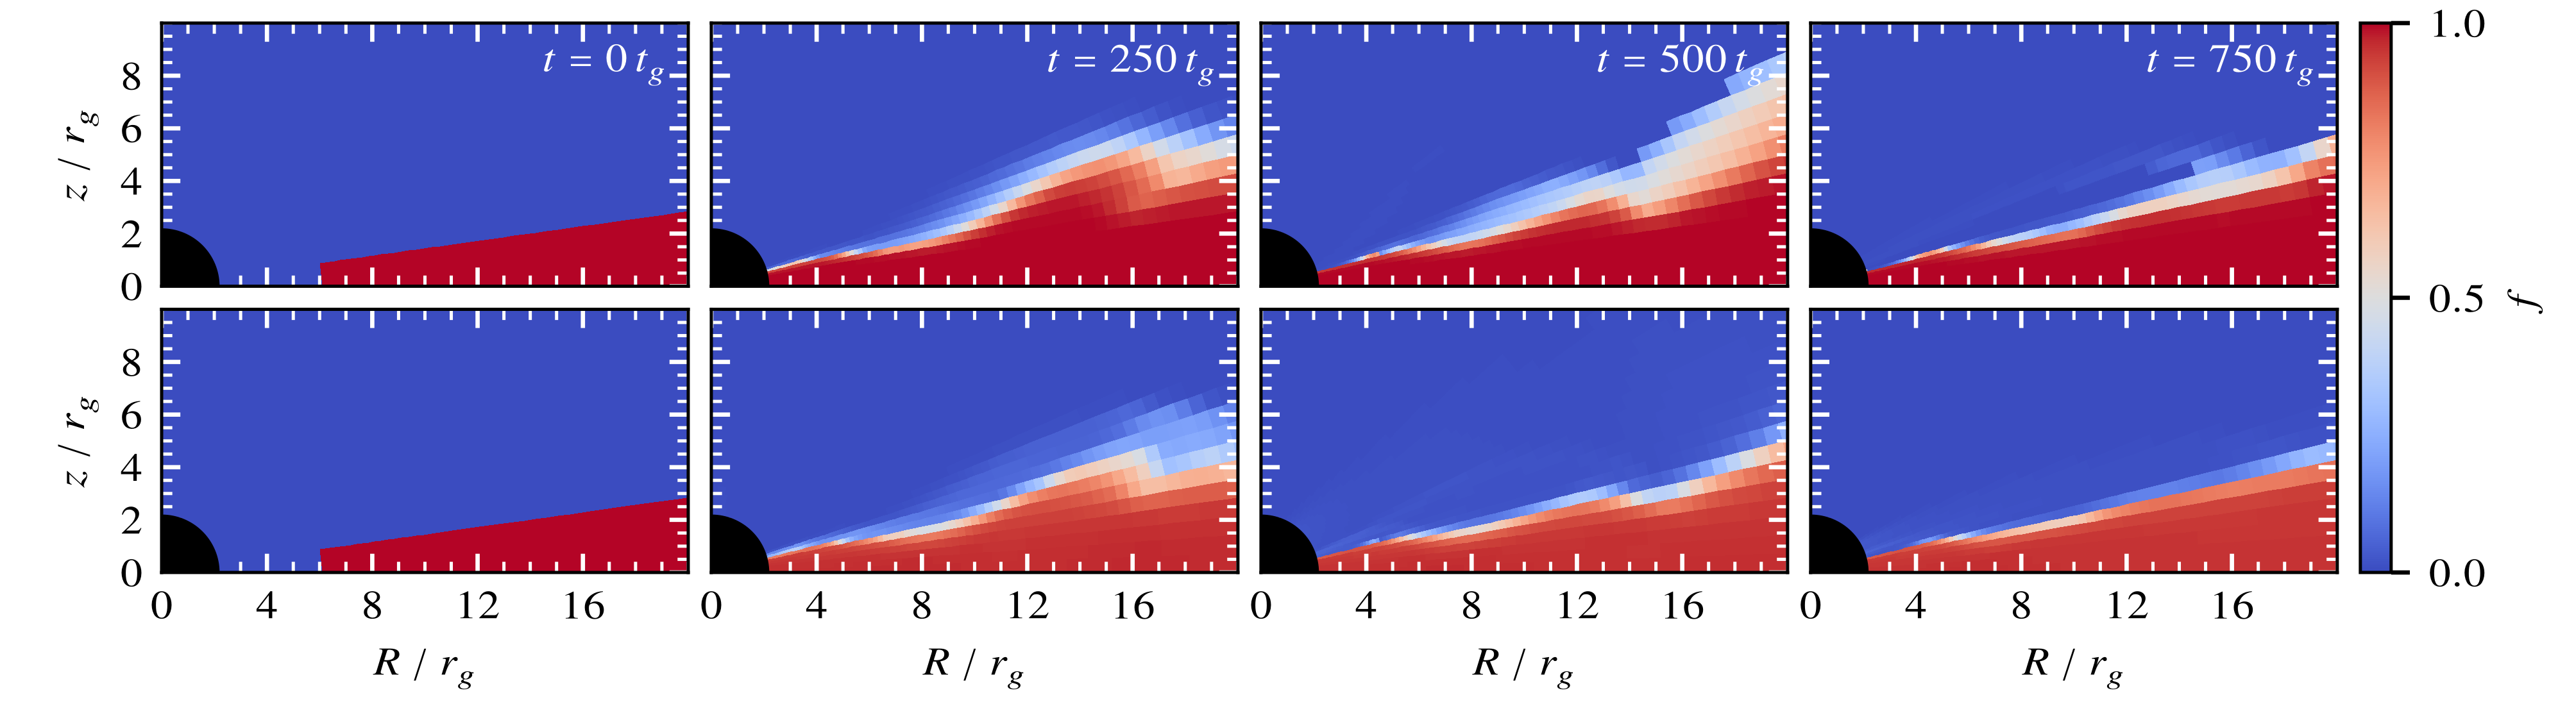
\includegraphics[width=\textwidth, draft=false]{plots/valid_hd_class_text.png}
		\caption{Passive tracer \textit{(top)} and DiskFraction \textit{(bottom)} in the classifier driven hydrodynamic run of
				 \Cref{fig:valid_rho} at the same times.}
		\label{fig:valid_class}
	\end{figure*}

	\begin{figure}[t]
		\centering
		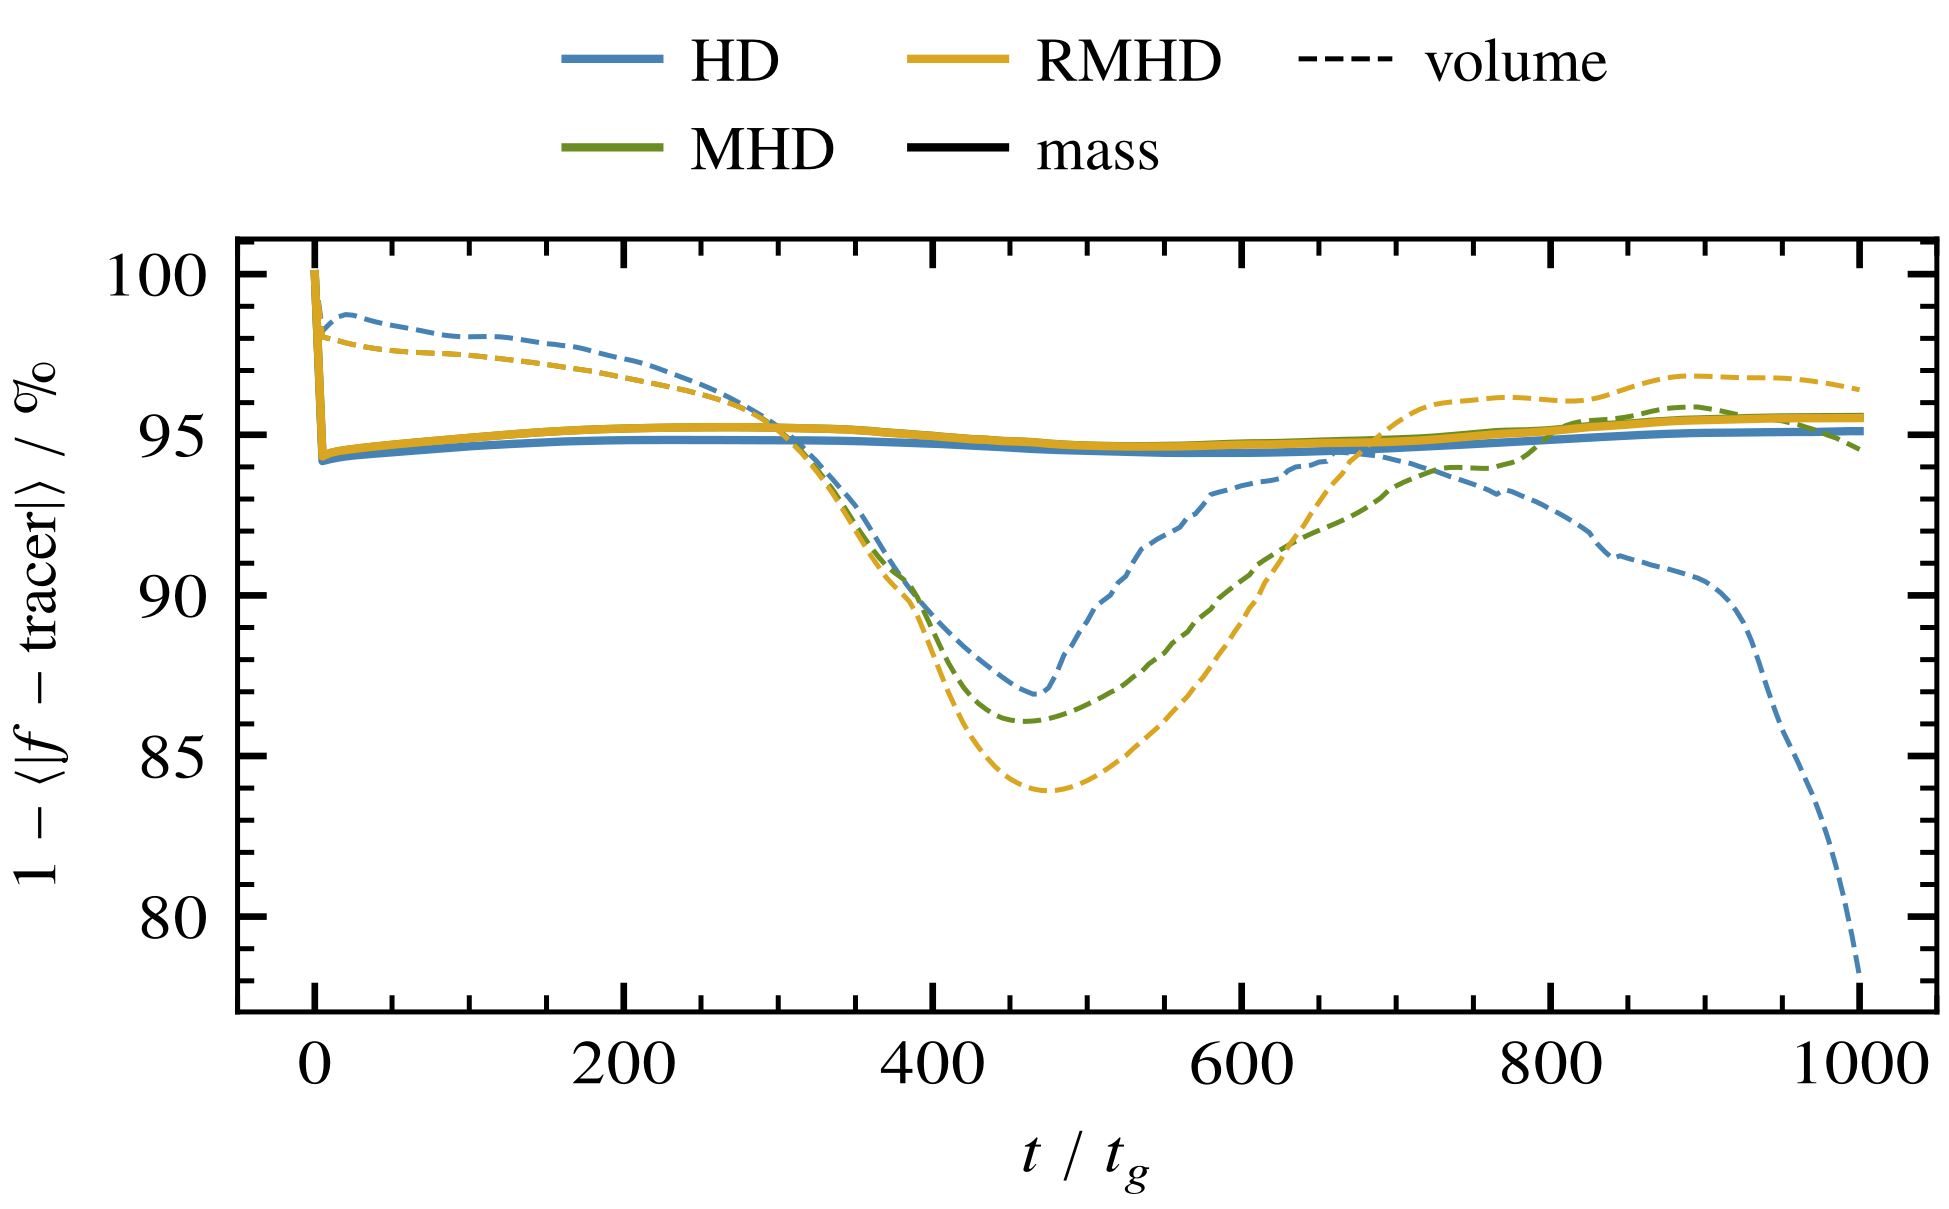
\includegraphics[width=\columnwidth, draft=false]{plots/valid_agreement_col.png}
		\caption{Agreement between DiskFraction and the passive tracer in the classifier driven runs without radiation, defined as
				 one minus the mean absolute difference over the domain, weighted by mass \textit{(solid)} and by volume
				 \textit{(dashed)}.}
		\label{fig:valid_agreement}
	\end{figure}

	\begin{figure*}[t]
		\centering
		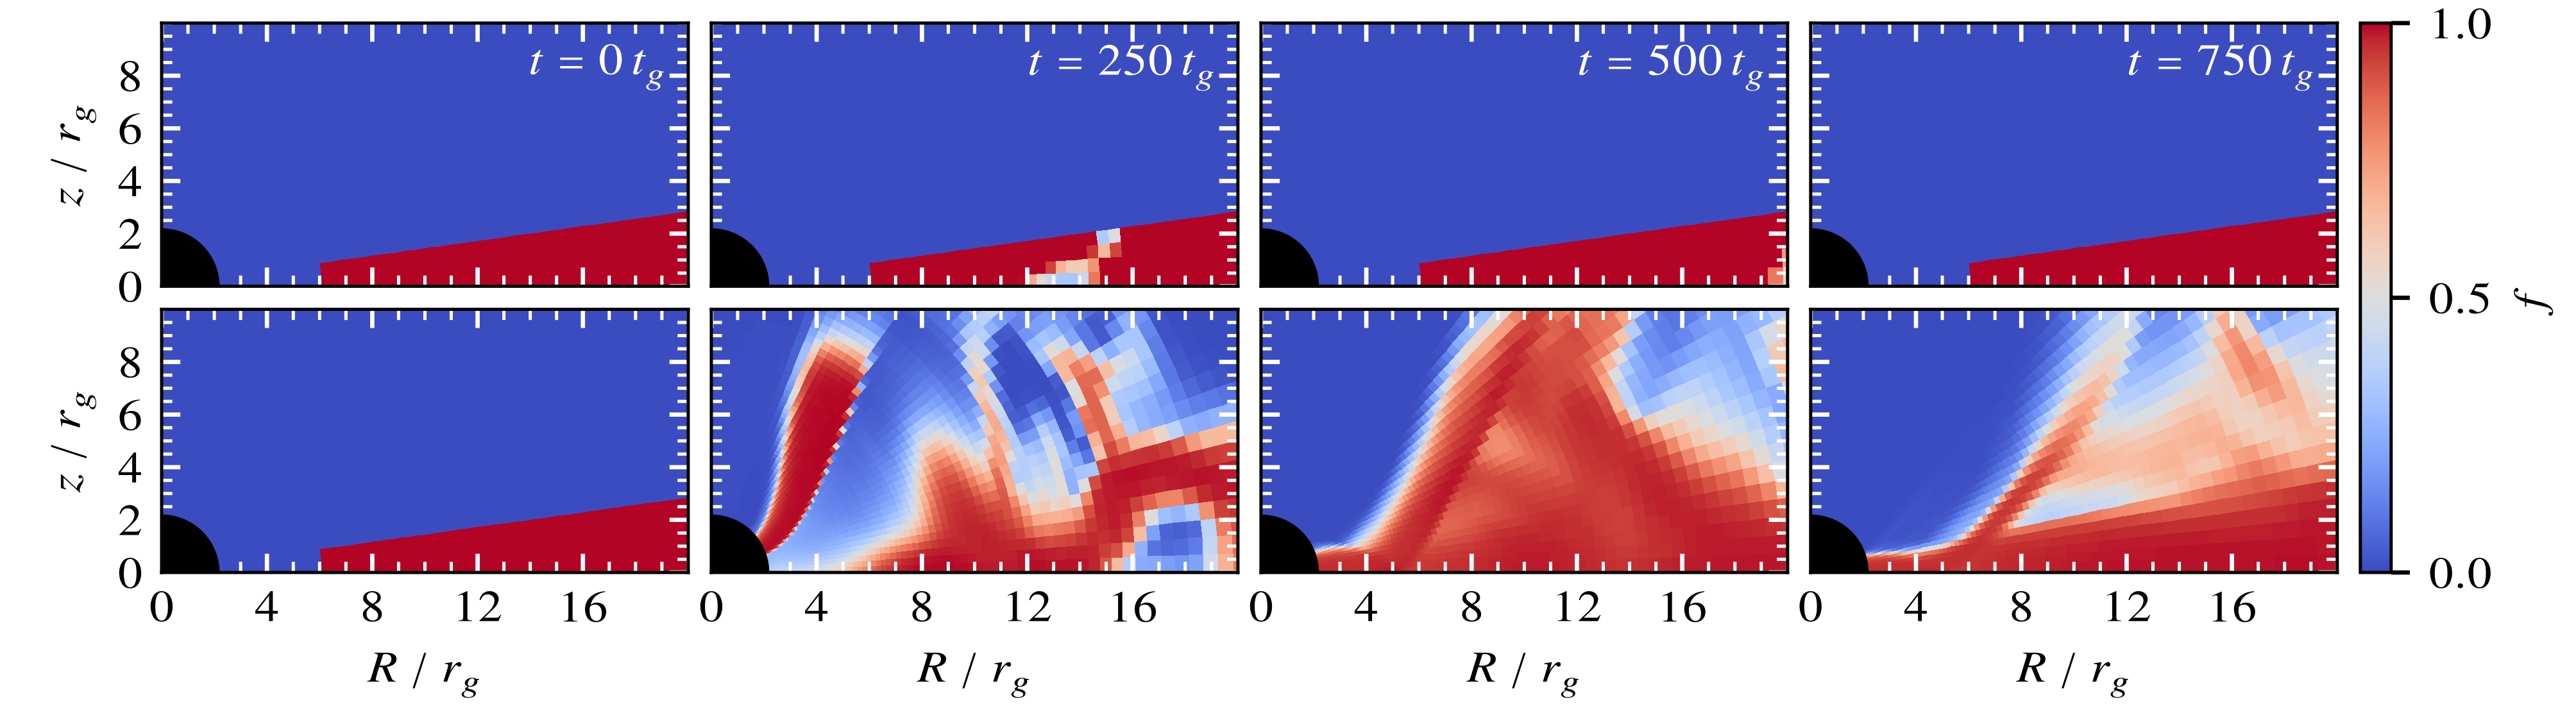
\includegraphics[width=\textwidth, draft=false]{plots/valid_rad_class_text.png}
		\caption{Passive tracer \textit{(top)} and DiskFraction \textit{(bottom)} in the first radiation run, in which DiskFraction
				 already drives the physics. The tracer keeps its initial distribution while the disk evolves.}
		\label{fig:valid_rad}
	\end{figure*}

	\section{Results}
	\label{sec:results}

	We now turn to the radiation runs with Compton coupling and the classifier. The run LR uses \num{90} by \num{45} cells and
	reaches $t = 5 \times 10^4$ in gravitational times, with outputs every \num{50} gravitational times. The run HR uses \num{120}
	by \num{90} cells and reaches $t = 4 \times 10^4$ with the same output cadence, which increases to every five gravitational
	times from $t = 3 \times 10^4$ onward for the wave analysis. Apart from the resolution, the two runs differ in the version of
	the classifier. LR still uses the first version described above, while HR uses the current version with all guards. Differences
	between the runs can therefore not be attributed to resolution alone. For the black hole mass of our setup, the run time of HR
	corresponds to about \num{230} days. The analysis methods are summarized in \Cref{app:methods}.

	\subsection{Evolution and Relaxation}

	In the first few hundred gravitational times, the disk adjusts to the radiation. It inflates, and a dense layer forms at its
	surface, which then breaks up, as shown in \Cref{fig:early}. After this, the two runs evolve differently, as
	\Cref{fig:relax_mass} shows. In HR, the disk is blown apart. Its mass falls from \num{132} to about \num{2} in units of
	$\rho_0 r_g^3$ by $t \approx 2000$ in gravitational times, and the disk stays fragmented until about $t = 10500$ before it is
	rebuilt by about $t = 15000$ and settles at a mass of about \num{18} in the same units. In LR, the disk mass instead declines smoothly from
	\num{143} to about \num{22} by $t \approx 5000$ without any breakup. We think this is most probably due to the stronger
	numerical viscosity, diffusivity and damping at lower resolution, which can smooth out the perturbations that grow into the
	breakup in HR, but the different classifier versions may also contribute. In both runs, the corona loses most of its mass
	early on and is not replenished, since the outer boundary blocks coronal inflow.

	To decide when a run has reached a steady state, we compare running means of the disk mass, the radiation energy, the
	accretion rate at the inner boundary and the luminosity at the outer boundary with their mean over the last fifth of the run.
	The steady state begins when all four stay within two standard errors of the reference, which happens at $t = 23725$ for HR
	and $t = 9225$ for LR in gravitational times. All averages in the following are taken over these windows, and within them
	the drift of the averages is consistent with zero.

	\begin{figure*}[t]
		\centering
		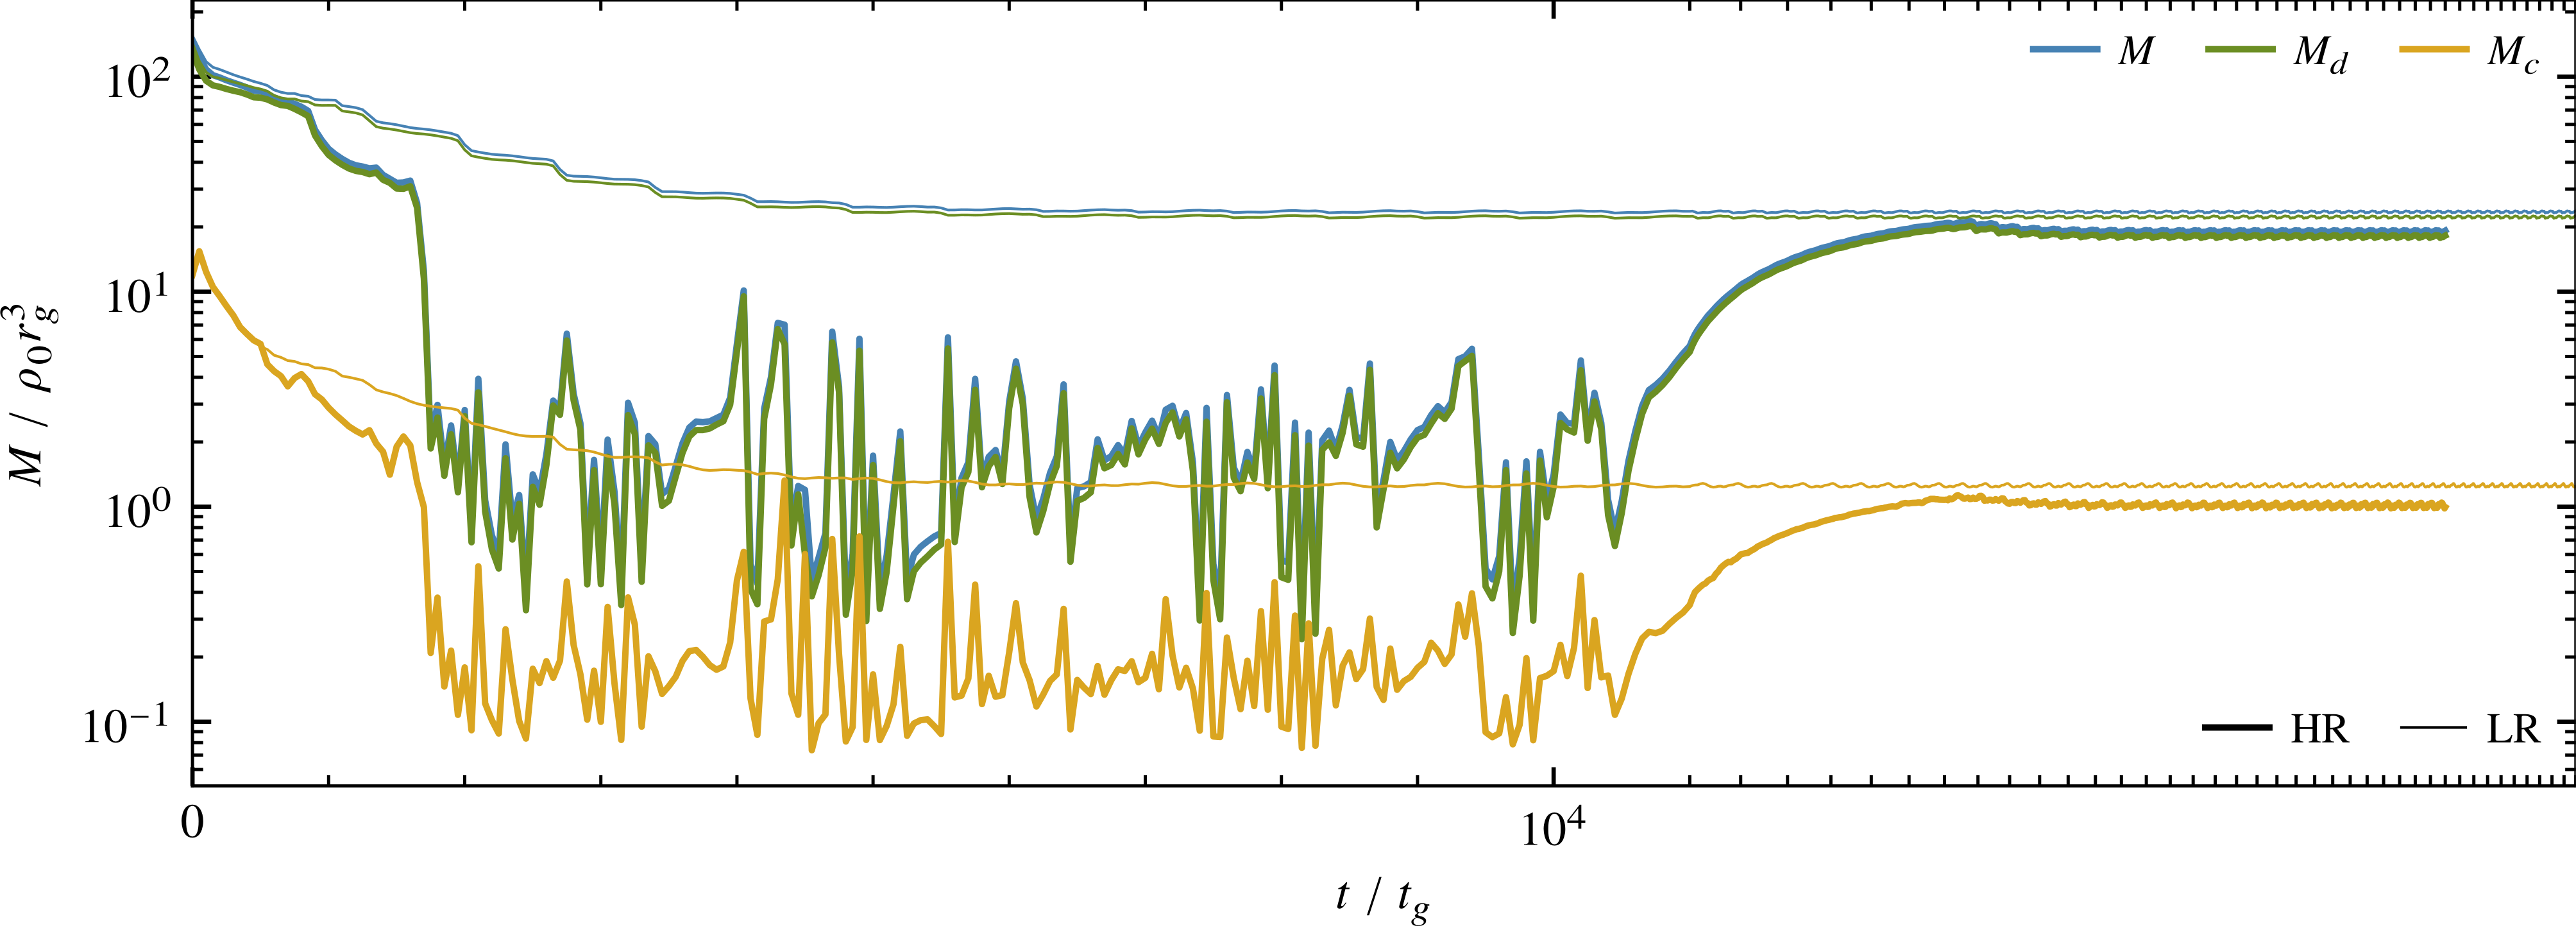
\includegraphics[width=\textwidth, draft=false]{plots/relax_mass_text.png}
		\caption{Total, disk and corona mass of both radiation runs, split by DiskFraction. The time axis is linear up to
				 $t = 1.1 \times 10^4$ and logarithmic beyond.}
		\label{fig:relax_mass}
	\end{figure*}

	\begin{figure*}[t]
		\centering
		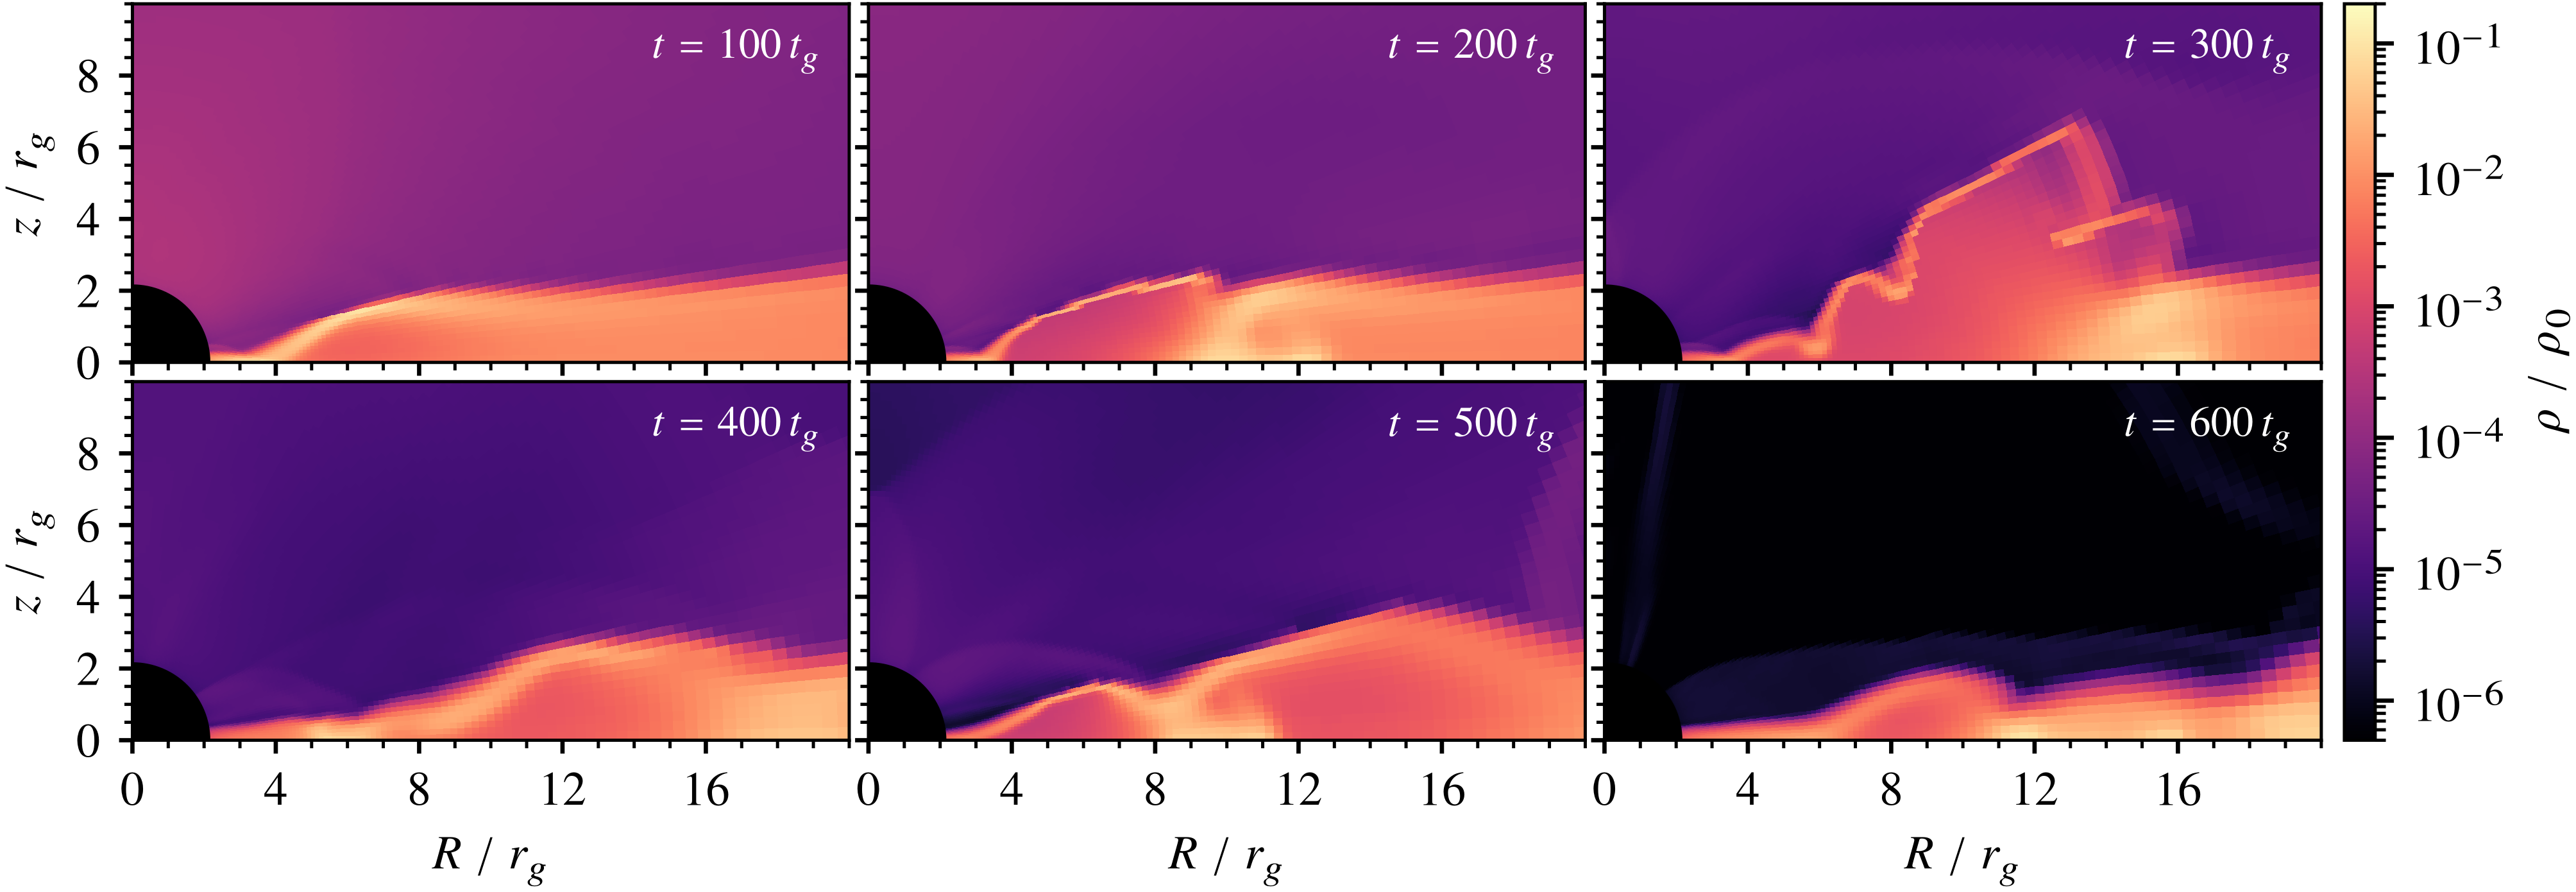
\includegraphics[width=\textwidth, draft=false]{plots/early_rho_text.png}
		\caption{Density in the early evolution of HR. The disk inflates and forms a dense surface layer that breaks up.}
		\label{fig:early}
	\end{figure*}

	\subsection{Steady State}

	\Cref{fig:domain} shows the initial density of HR and its average over the last \num{10000} gravitational times, together with
	the disk surface where $f = 0.5$ and the surface where the optical depth from the pole reaches unity. In the steady state, the
	disk is thinner than initially. At $R = 10$ its aspect ratio is about \num{0.057} in HR and \num{0.042} in LR, compared with
	\num{0.1} initially, which means that LR resolves the disk with only about one cell per scale height against about three in HR.

	\begin{figure*}[t]
		\centering
		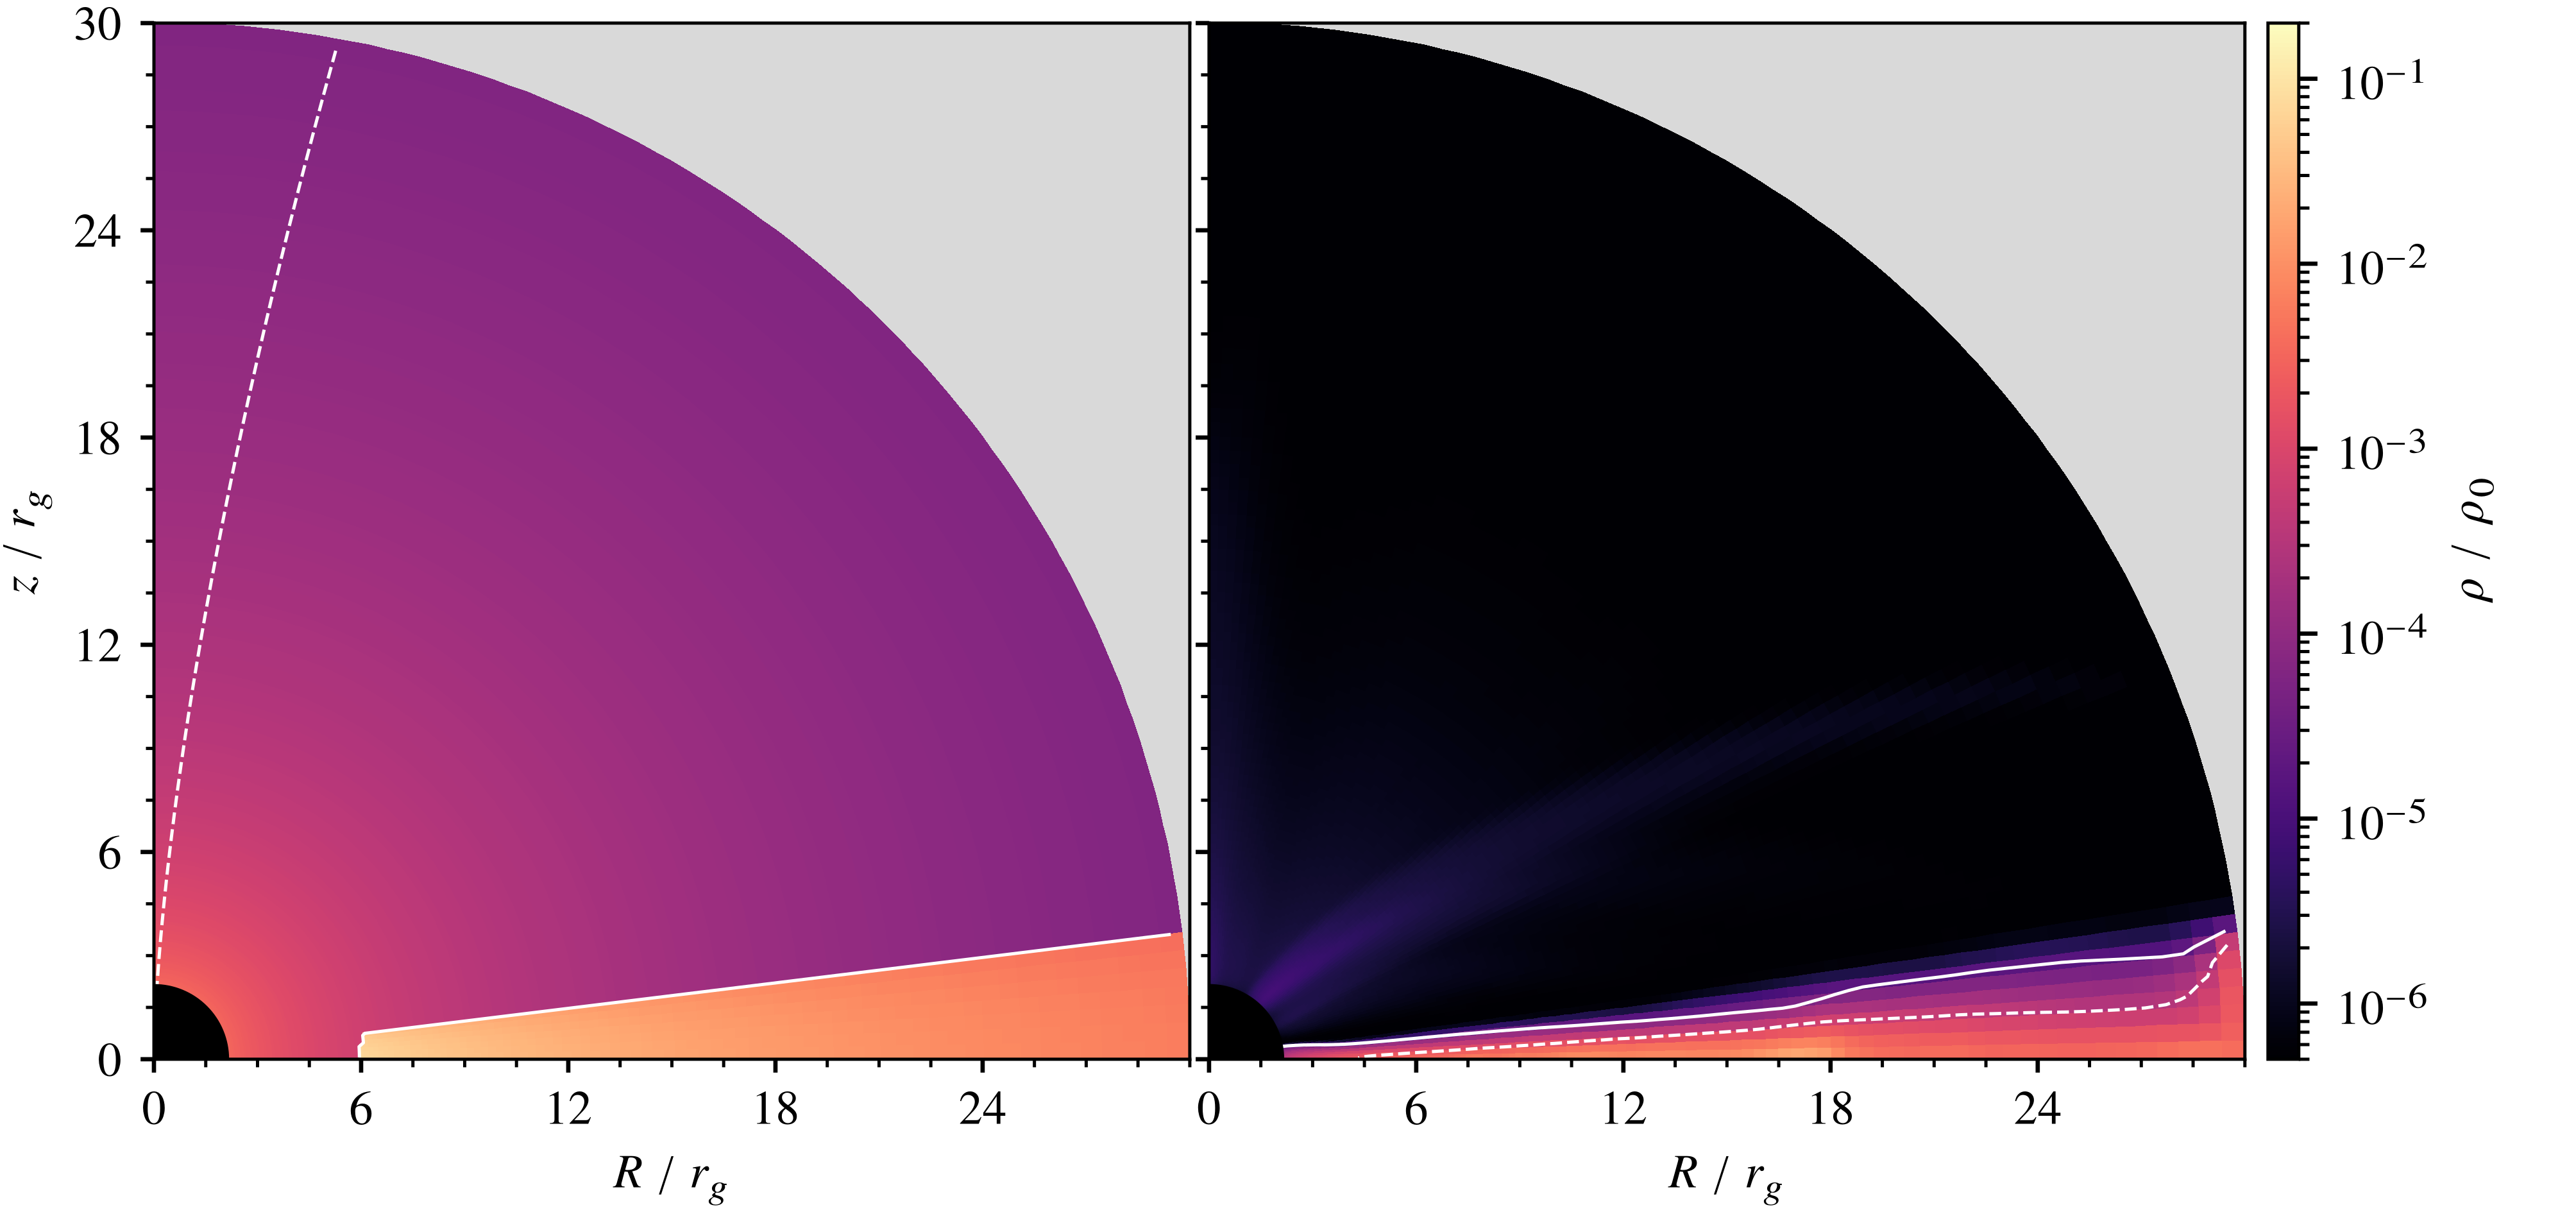
\includegraphics[width=\textwidth, draft=false]{plots/domain_rho_text.png}
		\caption{Density of HR initially \textit{(left)} and averaged over the last \num{10000} gravitational times
				 \textit{(right)}. White solid lines mark $f = 0.5$ and white dashed lines unit optical depth from the pole.}
		\label{fig:domain}
	\end{figure*}

	The accretion rate in \Cref{fig:mdot_sigma} is flat in radius out to about $r = 17$ in gravitational radii in both runs,
	so that the inner disk is in inflow equilibrium. Further out, the disk has not yet relaxed, which matches the estimate
	that viscous inflow reaches radii of about \num{26} and \num{30} within the run times of HR and LR. The mean accretion rate at
	the inner boundary is \num{0.073} times the Eddington rate in HR and \num{0.091} in LR, where the Eddington rate is defined
	with the efficiency $\eta = 1/16$ from above. This corresponds to about \num{0.30} and \qty{0.38}{\solarmass\per\year} respectively. The
	luminosity leaving the outer boundary is \num{0.056} and \num{0.070} times the Eddington luminosity, or about
	\qty{8.3e44}{\erg\per\second} and \qty{1.0e45}{\erg\per\second} for the two runs. The ratio of both gives a radiative efficiency
	of about \num{0.048} in both runs, somewhat below the value for a disk that radiates all its binding energy. This is
	plausible if part of the radiation is advected into the black hole or has not yet left the domain, but we have not
	measured these contributions separately.

	\begin{figure*}[t]
		\centering
		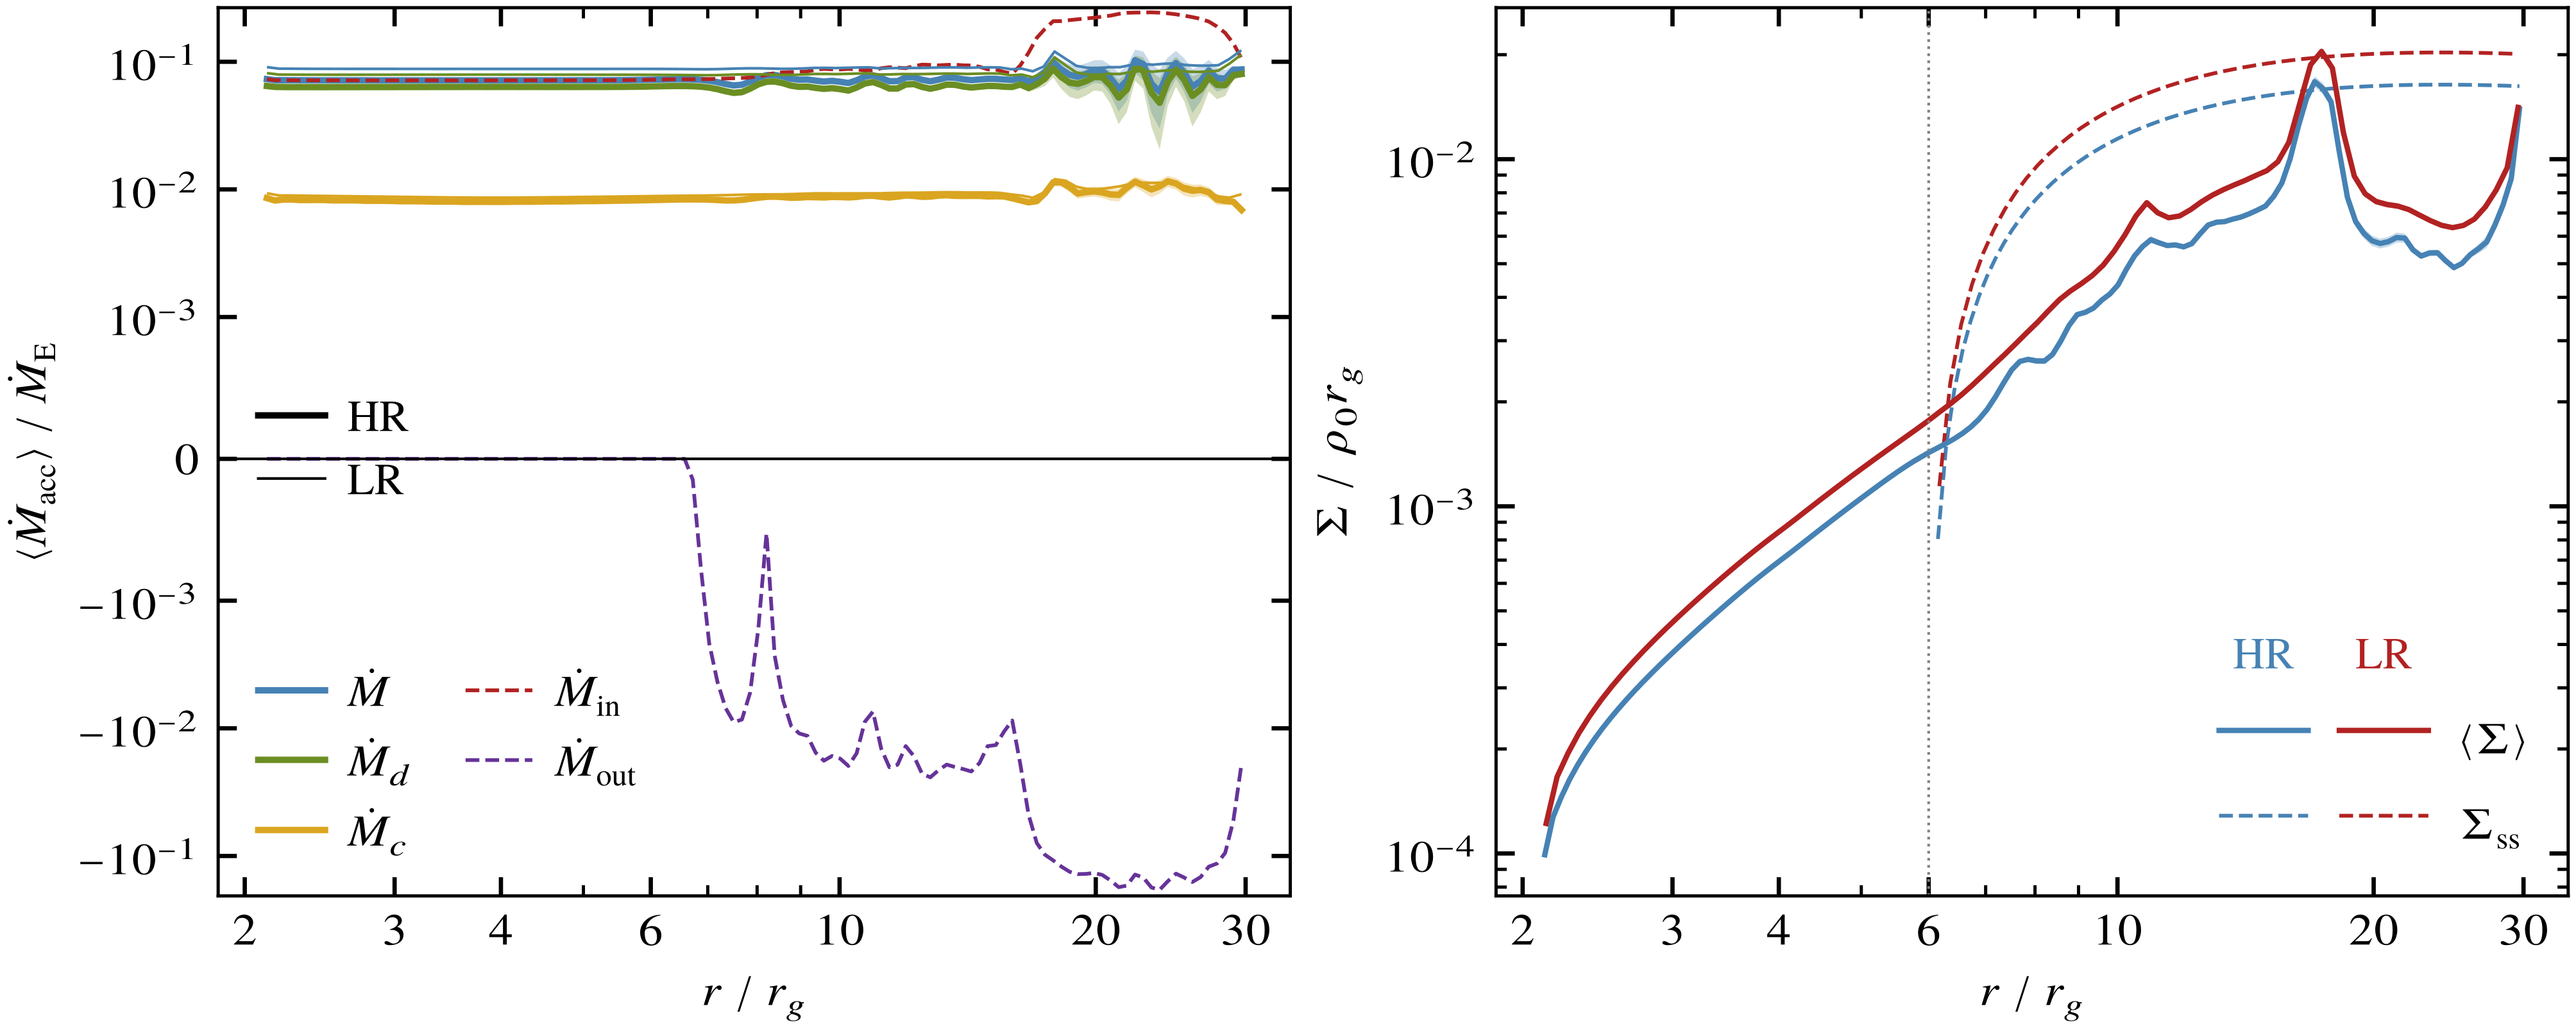
\includegraphics[width=\textwidth, draft=false]{plots/mdot_sigma_text.png}
		\caption{\textit{Left:} Time averaged accretion rate, positive for inflow, in total and split into disk and corona, as well as
				 the inflowing and outflowing parts. \textit{Right:} Time averaged surface density and the steady state profile
				 $\Sigma_\mathrm{ss}$ of \Cref{eq:sigma} for the measured accretion rate. Shaded bands show the standard errors of HR.}
		\label{fig:mdot_sigma}
	\end{figure*}

	For a steady thin disk with a stress free inner edge at six gravitational radii, the surface density follows
	\begin{equation}
		\Sigma_\mathrm{ss} = \frac{\dot M}{3 \pi \nu} \left(1 - \sqrt{\frac{6}{R}}\right)
		\label{eq:sigma}
	\end{equation}
	with the kinematic viscosity $\nu$ of our prescription in \Cref{app:equations}. The measured surface density in
	\Cref{fig:mdot_sigma} lies mostly below this profile, which means that angular momentum is transported more efficiently than
	the prescribed viscosity alone would allow. Inverting \Cref{eq:sigma} for an effective viscosity parameter gives values of about
	two to three times the prescribed $\alpha$ between $R = 10$ and $R = 20$ in both runs, as shown in \Cref{fig:alpha}. The
	additional transport may come from resolved flows such as the waves below, or from numerical effects, which we cannot
	separate here.

	\begin{figure}[t]
		\centering
		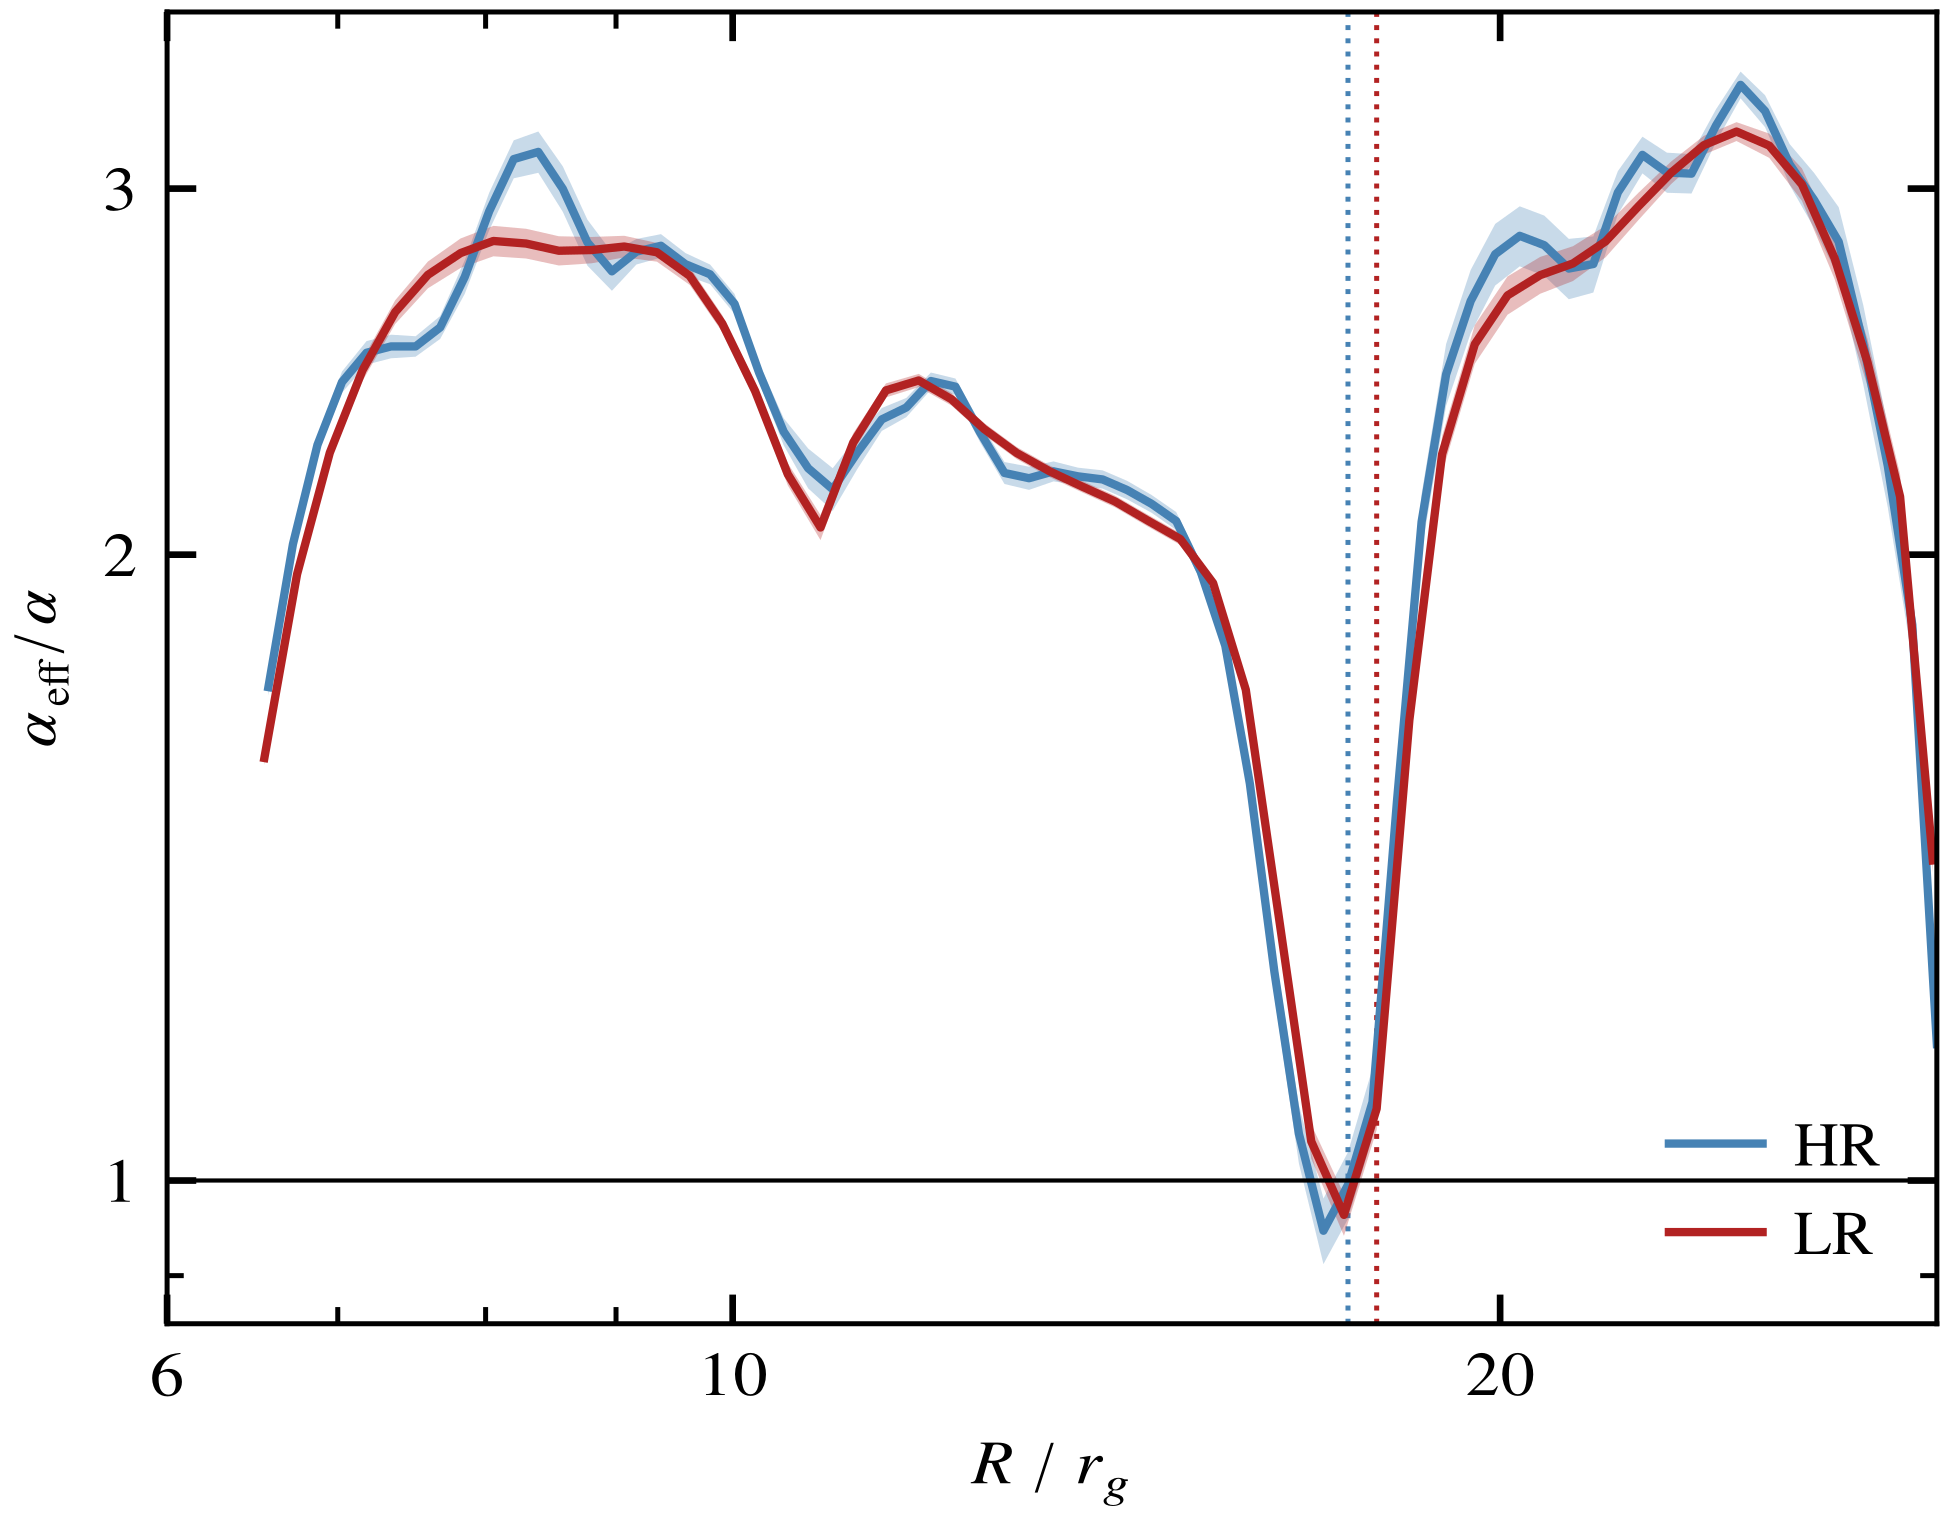
\includegraphics[width=\columnwidth, draft=false]{plots/alpha_col.png}
		\caption{Effective viscosity parameter from the measured accretion rate and surface density, relative to the prescribed
				 value. Dotted vertical lines mark the radius of inflow equilibrium of each run.}
		\label{fig:alpha}
	\end{figure}

	The thermal balance of the disk is dominated by Compton exchange. \Cref{fig:heating} compares the time in which viscous
	heating would double the thermal energy of the gas at the midplane with the corresponding cooling times by Compton exchange and
	by Kramers absorption. Between $R = 8$ and $R = 15$ the heating time is about \num{0.2} gravitational times, the Compton
	cooling time slightly shorter, and the Kramers cooling time two to three orders of magnitude longer. Heating and cooling
	therefore balance closely, with a ratio of about \num{0.8} to \num{0.9} of heating to cooling, and the gas stays coupled to the
	radiation on a time far shorter than the orbital time.

	\begin{figure*}[t]
		\centering
		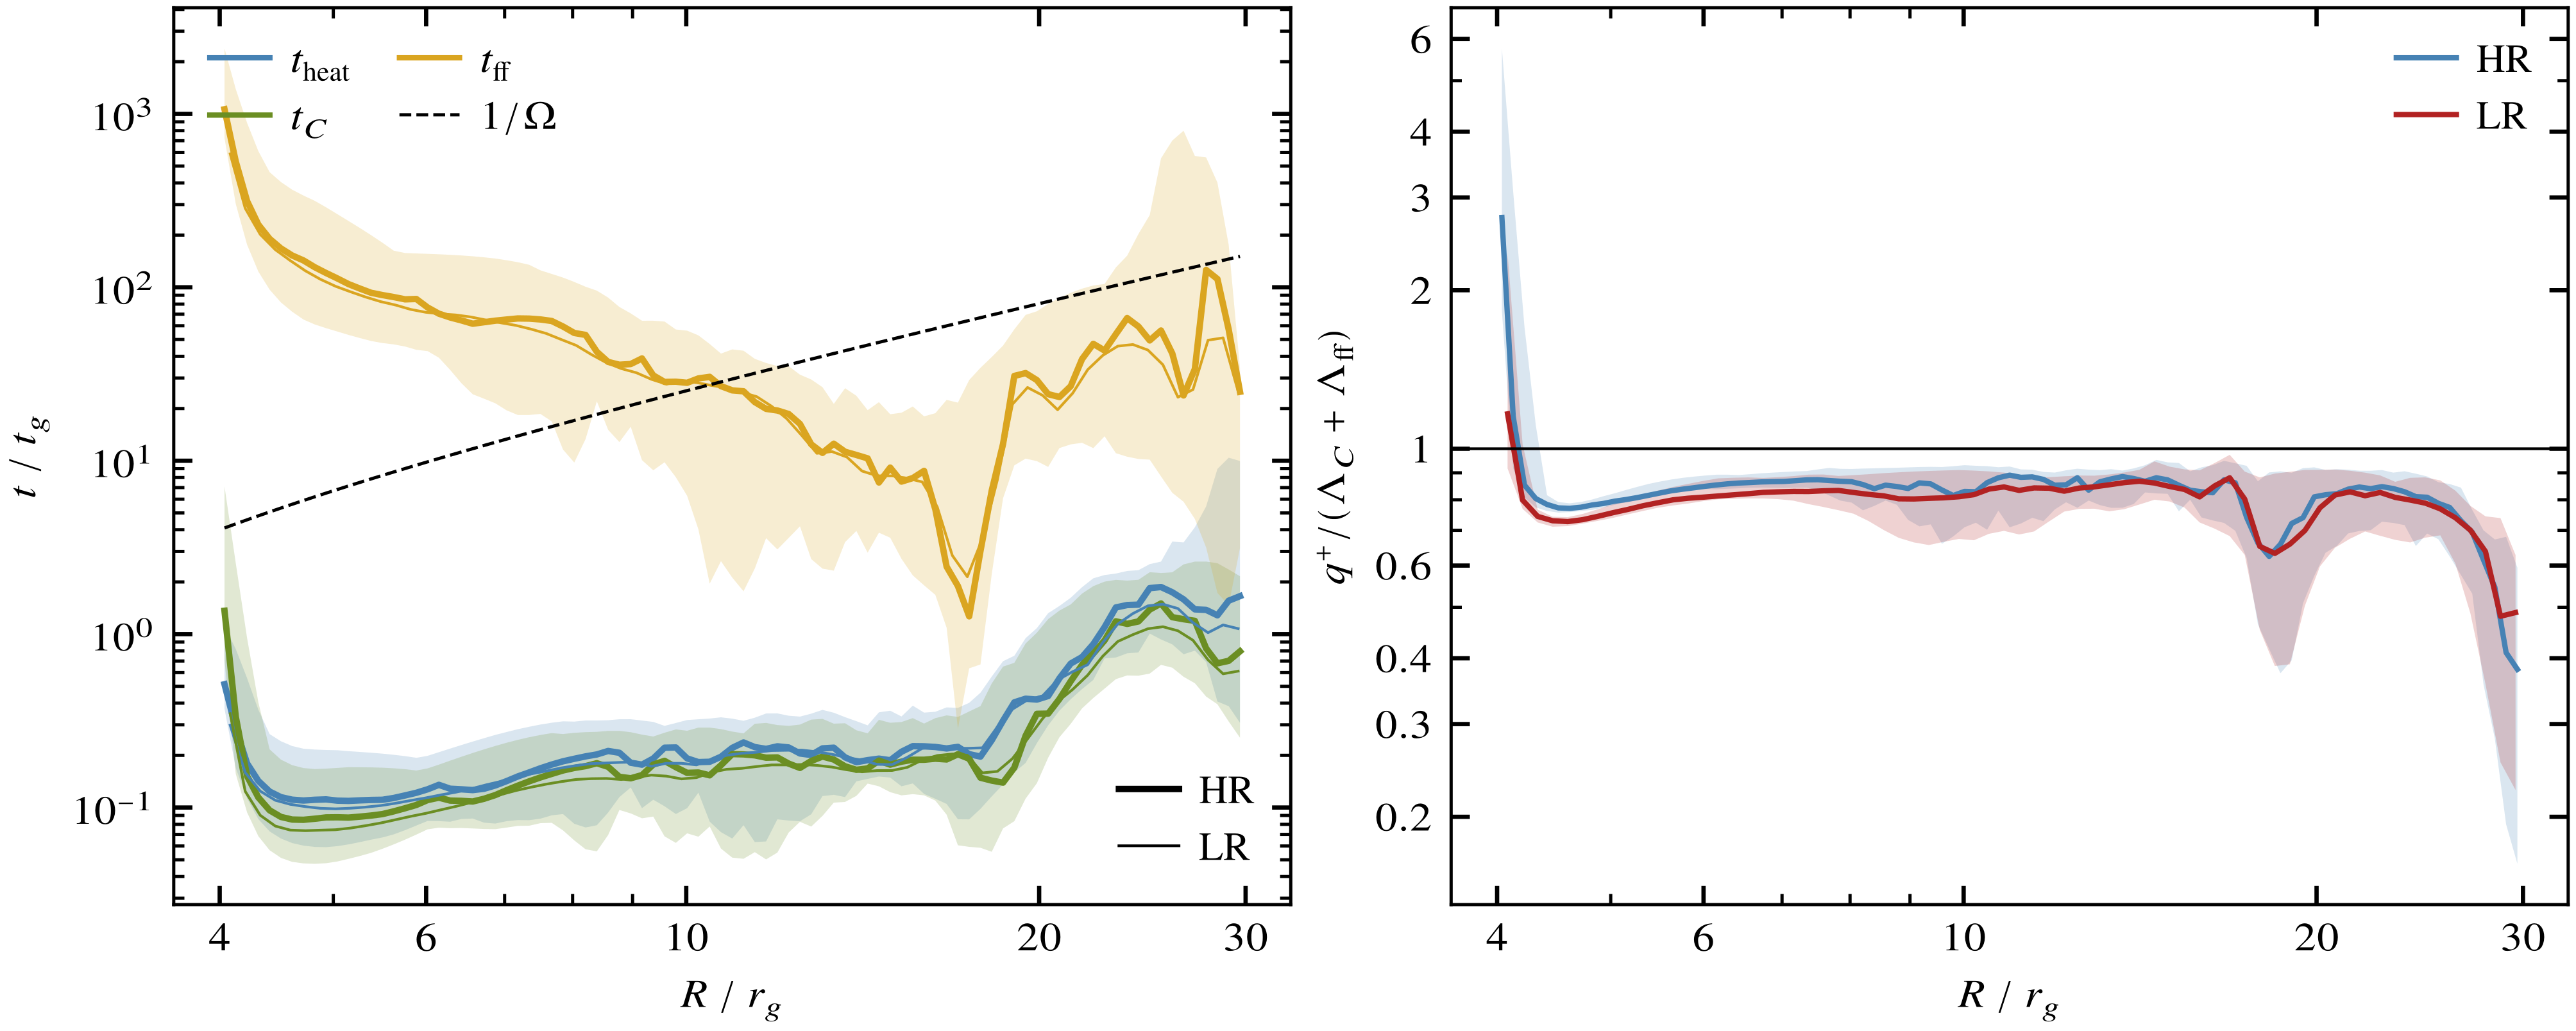
\includegraphics[width=\textwidth, draft=false]{plots/heating_text.png}
		\caption{\textit{Left:} Midplane times for viscous heating, Compton cooling and Kramers cooling, with the inverse orbital
				 frequency for comparison. Lines show medians over the steady state and bands the range between the 16th and 84th
				 percentiles for HR. \textit{Right:} Ratio of viscous heating to radiative cooling at the midplane.}
		\label{fig:heating}
	\end{figure*}

	\subsection{Outward Density Waves}

	Both runs show quasiperiodic density waves in the steady state. In the relative surface density perturbation of
	\Cref{fig:delta} they appear as ridges that start near the innermost stable orbit and travel outward to radii of about
	\num{17} and beyond. Power spectra of these perturbations peak at a frequency of about \num{2.9e-3} per gravitational time
	in both runs, which corresponds to a period of about \num{349} gravitational times or about two days for our black hole mass.
	The phase of the perturbation at this frequency grows steadily with radius, as shown in \Cref{fig:phase_speed}, so the
	waves propagate outward with a phase speed of about \num{0.019} times the speed of light between radii of about \num{4}
	and \num{17} in both runs. In HR, this is about \num{2.2} times the adiabatic sound speed including radiation pressure and
	about \num{6.5} times the sound speed of the gas alone. The waves are therefore not plain sound waves, and we have not
	identified their nature. That the period is the same in both runs, despite their different resolution and classifier
	version, suggests that it is set by the setup rather than by numerics, possibly by the inner boundary or the fixed
	sound speed in the viscosity, but this remains to be tested.

	\begin{figure*}[t]
		\centering
		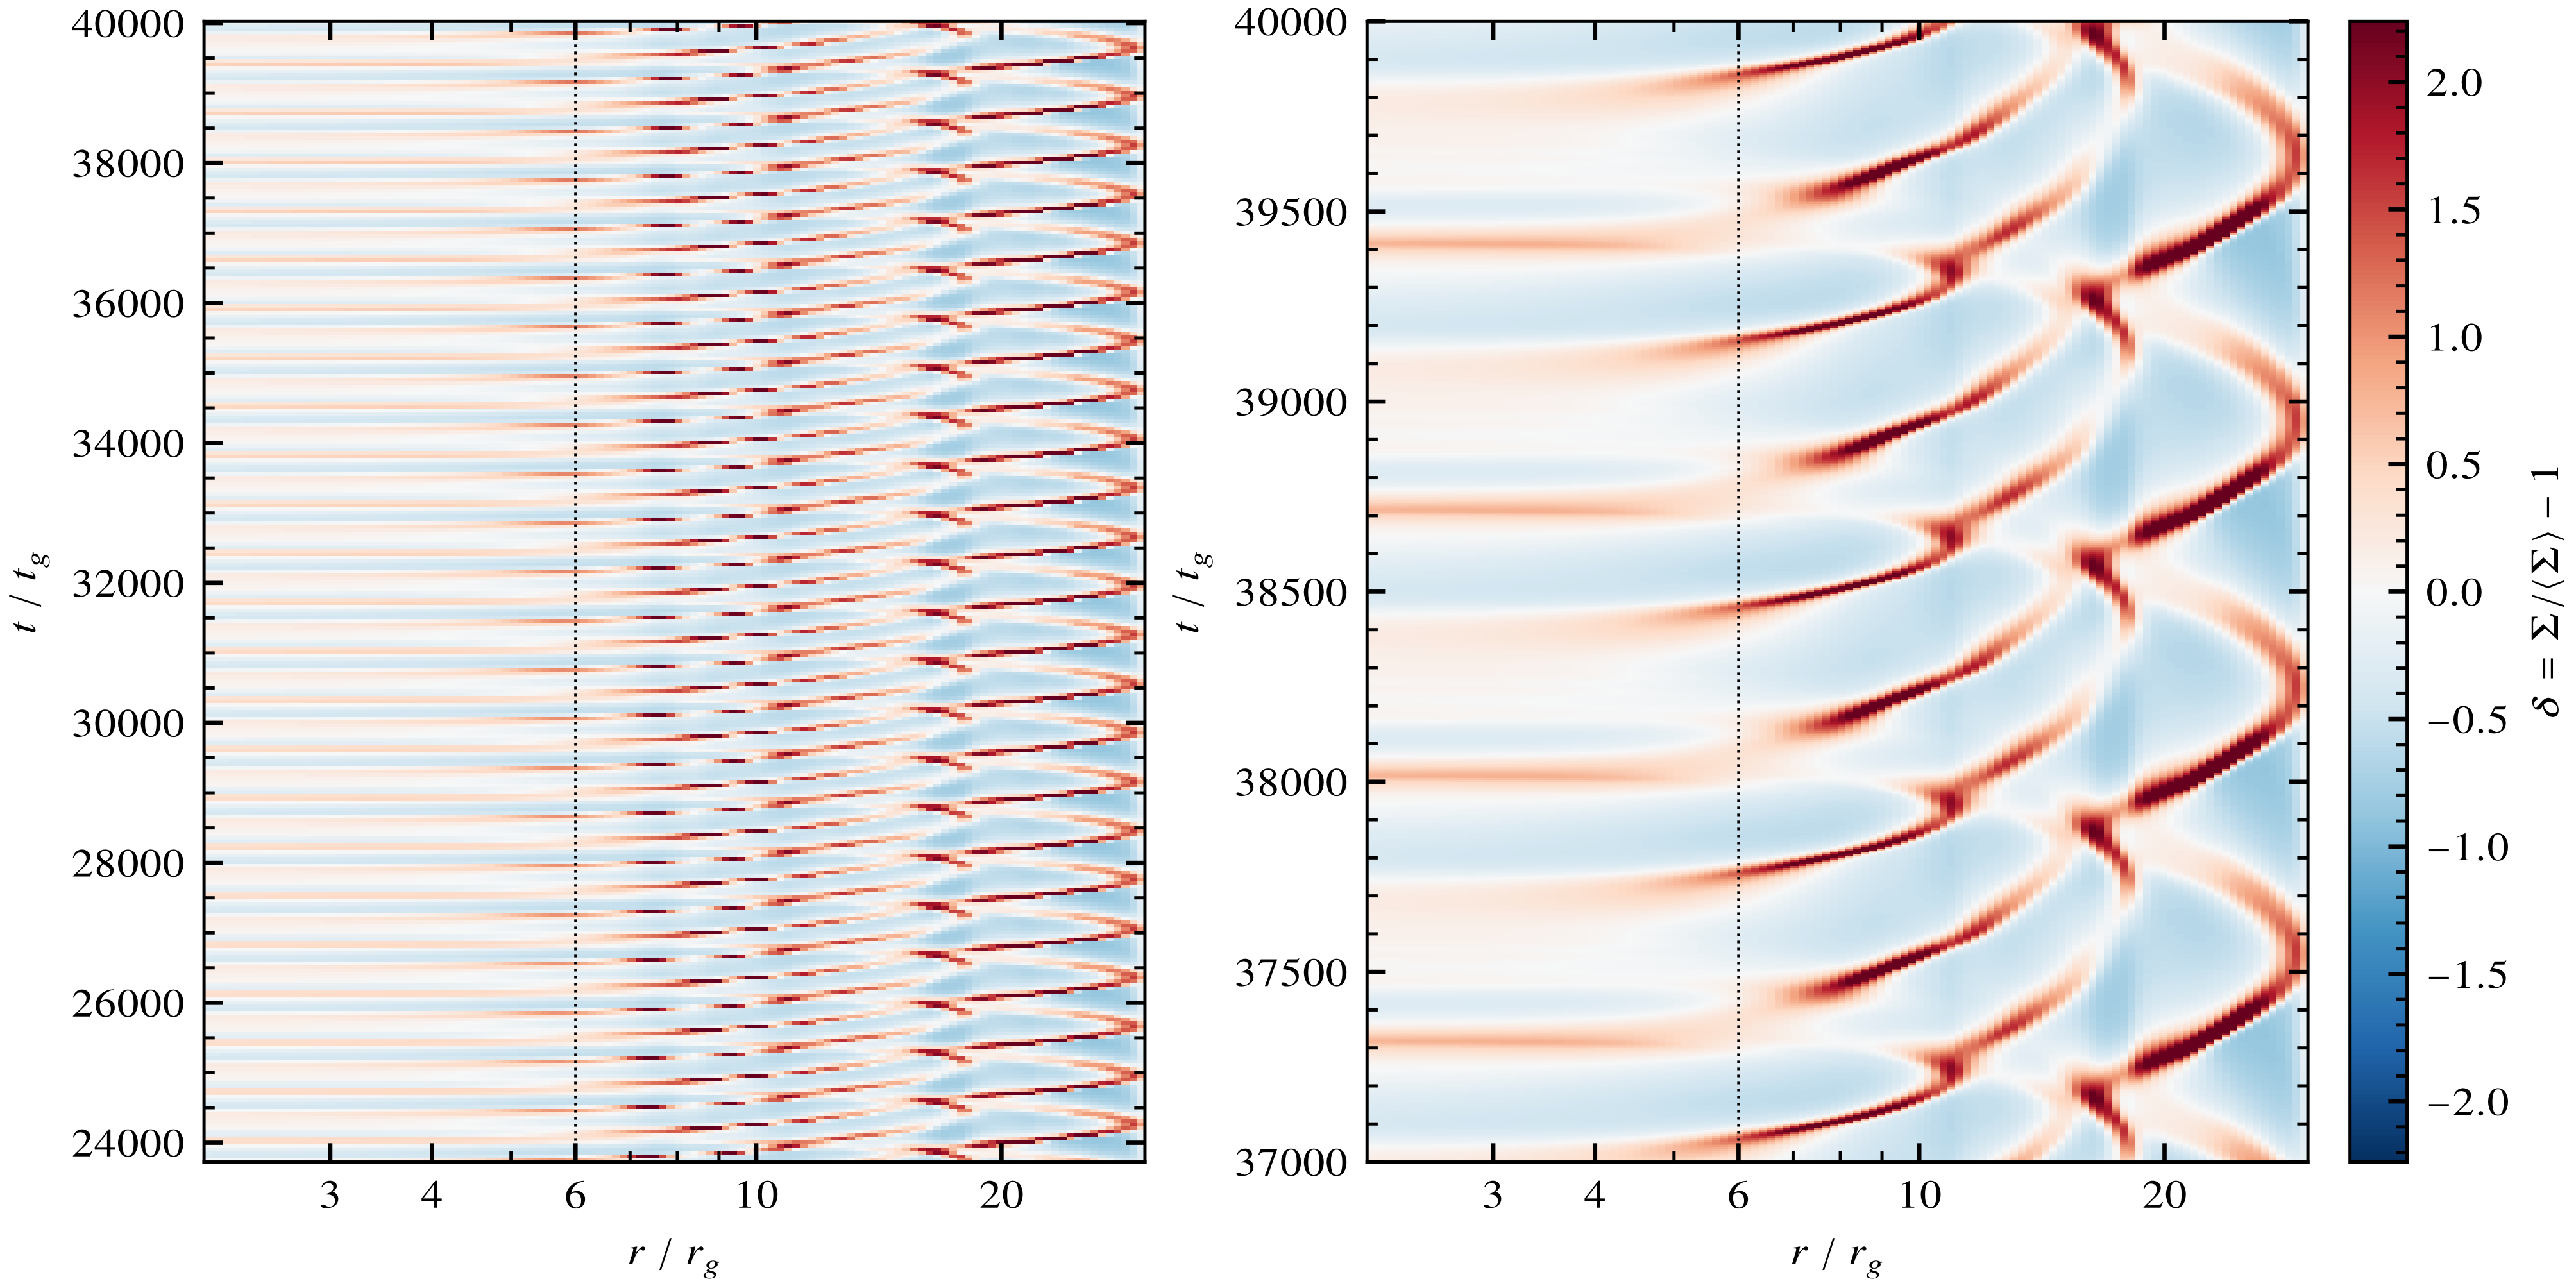
\includegraphics[width=\textwidth, draft=false]{plots/spacetime_delta_text.png}
		\caption{Relative surface density perturbation of HR in the steady state, at the regular output cadence \textit{(left)} and
				 at the dense cadence over the last \num{3000} gravitational times \textit{(right)}. The dotted line marks the innermost
				 stable orbit.}
		\label{fig:delta}
	\end{figure*}

	\begin{figure*}[t]
		\centering
		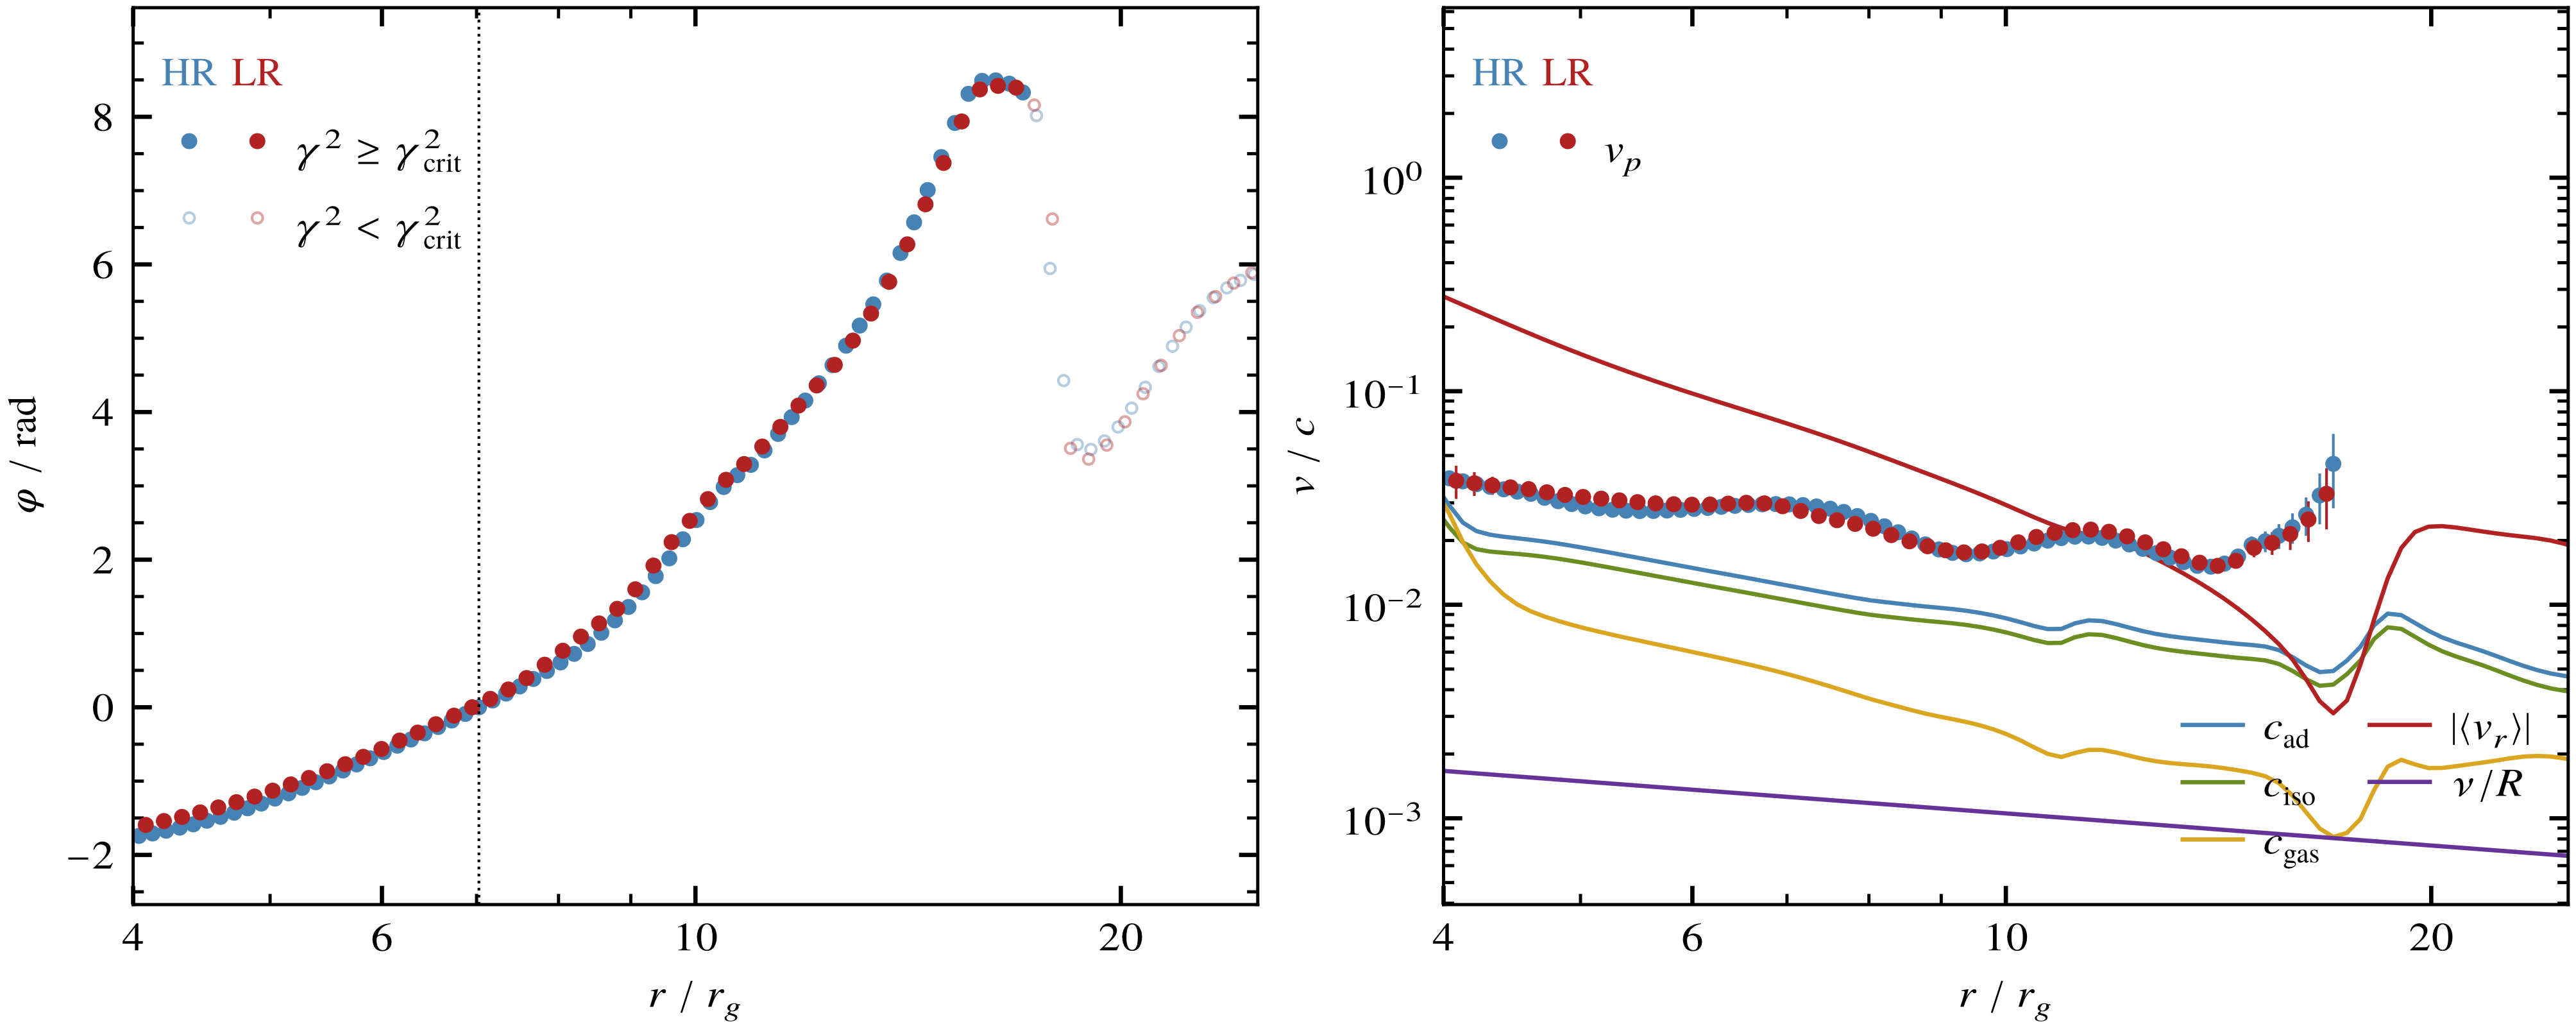
\includegraphics[width=\textwidth, draft=false]{plots/phase_speed_text.png}
		\caption{\textit{Left:} Phase of the surface density perturbation at the peak frequency relative to the reference radius
				 \textit{(dotted)}. Filled points have a significant coherence with the reference. \textit{Right:} Local phase speed
				 compared with the adiabatic, isothermal and gas sound speeds, the mean radial velocity and the viscous speed.}
		\label{fig:phase_speed}
	\end{figure*}

	\subsection{Mid Altitude Inflow Stream}

	Most of the accretion happens close to the midplane. In the steady state of HR, half of the net inflow passes within about
	one to three degrees of the midplane and nine tenths within about five to eight degrees at most radii, with the radius \num{10} in HR as an exception at about
	twenty degrees, while the disk surface
	sits between about five and nine degrees, so that about \num{90} percent of the inflow passes through the disk. Above the disk,
	the angular distribution of the inflow in \Cref{fig:angular} shows a second, much weaker maximum between about \num{20} and
	\num{50} degrees of elevation, at about a thousandth of the midplane value per degree. It belongs to a faint stream of gas
	falling toward the black hole at intermediate altitudes, which is also visible as a diagonal feature in the averaged density of
	\Cref{fig:domain}. This stream may well be an artifact of the setup. The corona starts in Newtonian hydrostatic equilibrium
	but evolves in the deeper pseudo potential, and the outer boundary changes its treatment of inflow at intermediate latitudes.
	We have not tested either explanation.

	\begin{figure}[t]
		\centering
		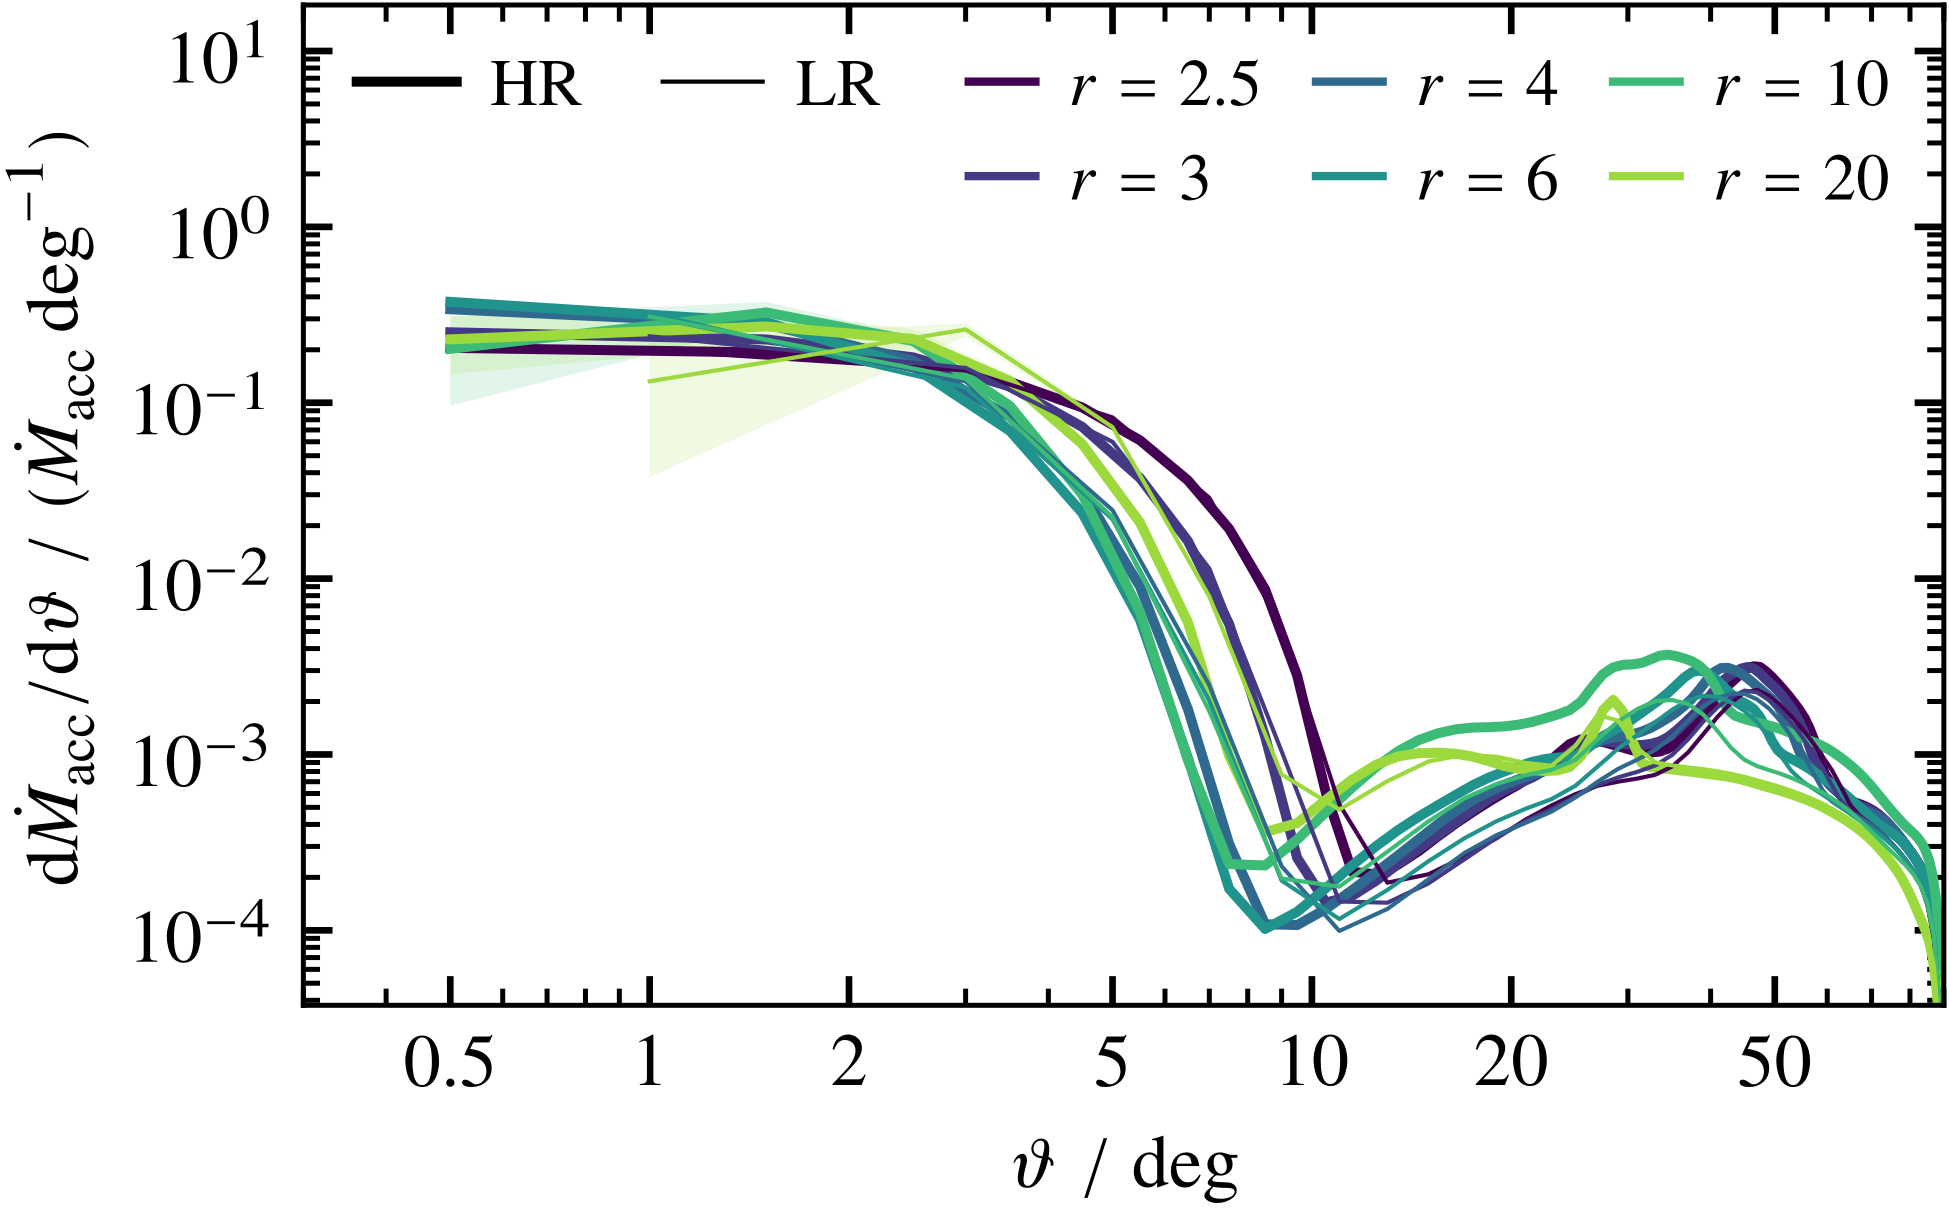
\includegraphics[width=\columnwidth, draft=false]{plots/angular_mdot_dist_col.png}
		\caption{Distribution of the time averaged net inflow over elevation above the midplane at several radii, normalized to the
				 total inflow at each radius.}
		\label{fig:angular}
	\end{figure}

	\subsection{Resolution Comparison}

	\Cref{tab:runs} summarizes the main quantities of both runs. The efficiency, the radius of inflow equilibrium and the wave properties agree within a few percent, while the accretion
	rate and luminosity of LR are about a quarter higher, its disk is thinner, and it survives the early evolution without breaking up. Since
	the classifier version changes together with the resolution, we cannot say which of these differences are due to resolution.

	\begin{table}[t]
		\centering
		\caption{Steady state quantities of both radiation runs. Times are in gravitational times, rates in Eddington units and radii in gravitational radii.}
		\begin{tabular}{l r r}
			\toprule
			Quantity & HR & LR \\
			\midrule
			Cells                     & $120 \times 90$ & $90 \times 45$ \\
			Classifier                & current         & first \\
			Steady state from         & \num{23725}     & \num{9225} \\
			Accretion rate            & \num{0.073}     & \num{0.091} \\
			Luminosity                & \num{0.056}     & \num{0.070} \\
			Efficiency                & \num{0.048}     & \num{0.049} \\
			Equilibrium radius        & \num{17.4}      & \num{17.9} \\
			Aspect ratio at 10        & \num{0.057}     & \num{0.042} \\
			Cells per scale height    & \num{3.3}       & \num{1.2} \\
			Wave period in $t_g$      & \num{349}       & \num{349} \\
			Phase speed in $c$        & \num{0.0190}    & \num{0.0195} \\
			\bottomrule
		\end{tabular}
		\label{tab:runs}
	\end{table}

	\section{Discussion and Outlook}
	\label{sec:discussion}

	Several features of the setup limit how far the results can be interpreted physically. The most important one concerns the
	viscosity. Its sound speed is not taken from the evolving gas but from the initial disk profile at the same position, so it
	does not depend on pressure. The stress therefore cannot grow when the disk heats up, which removes exactly the feedback
	that drives the thermal and viscous instability of radiation pressure dominated disks \cite{ligh1974, shak1976}. The stability
	of our steady states is thus no test of this instability.

	The boundaries also affect the results. The disk reinjected at the outer boundary and the blocked coronal inflow set the
	supply of gas, the corona drains early and is not replenished, and the inflow stream above may originate there. The mass
	budget of the steady state does not close either. The change of enclosed mass and the integrated fluxes through the
	boundaries differ by about three percent between the radii \num{2.5} and \num{25} and by about \num{18} percent for the full
	domain, far beyond the sampling error and with a sign that the density floors, which can only add mass, cannot explain. This
	points to the boundary treatment or to the cell centered fluxes used in our diagnostic, as discussed in
	\Cref{app:methods}.

	Further limitations concern the physics. The corona reaches temperatures of up to about \qty{1e11}{\kelvin} in our runs, where $k_B T$ is
	about \num{46} times the electron rest energy, and such temperatures are probably too high for our setup to be trusted. The
	nonrelativistic Compton rate is far outside its validity there, which is why we hold it fixed above \qty{1e9}{\kelvin} in the opacity model. The
	setup also includes neither relativistic corrections to Compton scattering nor pair production, which would both matter at
	these temperatures. With Newtonian dynamics in the pseudo potential, the plunging gas inside about four gravitational radii
	reaches radial velocities of several times the speed of light and rotation velocities of about \num{1.4} times the speed of
	light near the inner boundary. The radiation there is decoupled from the gas to keep the nonrelativistic radiation module
	stable, but the dynamics of this region are unphysical. Finally, the simulations are axisymmetric and hydrodynamic, so
	turbulence driven by the magnetorotational instability is replaced by the alpha prescription, and LR resolves the disk
	vertically with only about one cell per scale height.

	Natural next steps are a viscosity with a sound speed derived from the evolving total pressure, which would allow the disk to
	become thermally unstable, a larger domain that moves the outer boundary away from the region of interest, and an initial disk
	that is better suited to radiation pressure dominated accretion, such as a disk built from the standard thin disk solution
	\cite{shak1973}.

	\section{Conclusions}

	We adapted a viscous and resistive star disk setup in PLUTO to a nonrotating supermassive black hole and added radiation with
	Compton coupling. Since the passive tracer that restricts the disk physics fails once radiation is enabled, we developed the
	DiskFraction classifier, which reproduces the tracer in runs without radiation, follows the disk with radiation, and in its
	current version repairs its own errors. With it, two radiation runs at different resolutions reach steady states at roughly a
	tenth of the Eddington rate, in which Compton exchange balances viscous heating closely, the effective viscosity exceeds the
	prescribed one by a factor of two to three, and quasiperiodic density waves with a period of about \num{350} gravitational
	times travel outward. Whether these features and the weak inflow stream at intermediate altitudes are physical or artifacts of
	the fixed sound speed, the boundaries and the missing high temperature physics has to be tested with the improvements outlined
	above.

	\newpage
	\renewcommand{\thesubsection}{\Alph{subsection}}
	\label{sec:appendix}
	\twocolumn[{
		\printbibliography

		\section*{Appendix}

		\pagenumbering{roman}
		\setcounter{page}{1}

		This section contains the equations of secondary importance, the analysis methods and supplementary graphics. All
		simulation setups, the analysis notebook and the plotting script for this report are found in this
		\href{https://github.com/fritzali/notes/tree/main/CAMK}{repository}.
		\vspace{\baselineskip}
	}]

	\subsection{Model Equations}
	\label{app:equations}

	All quantities in this section are in code units unless stated otherwise. The corona starts with the density
	$\rho = \rho_c r^{-3/2}$ and pressure $p = 0.4 \rho_c r^{-5/2}$ where $\rho_c = 0.01$ is assumed. With the function
	\begin{equation}
		C = \frac{2}{5 \epsilon^2} \left(\frac{1}{r} - \frac{1 - 5 \epsilon^2 / 2}{R}\right)
	\end{equation}
	the disk has the pressure $p = \epsilon^2 C^{5/2}$ and density $\rho = C^{3/2}$ wherever its pressure exceeds that of the
	corona and $R > 6$ holds. Its velocities follow the same analytic solution \cite{kluz2000}. In the radiation runs, the pressure of the analytic disk is
	shared between gas and radiation at a common temperature, which makes the initial disk radiation pressure dominated.

	The dynamic shear viscosity is
	\begin{equation}
		\eta_\nu = \frac{2}{3} \alpha \rho \epsilon^2 C R^{3/2} f
	\end{equation}
	where $\epsilon^2 C$ is the squared sound speed of the initial disk at the position of the cell, which is fixed in time. At
	the midplane, this gives the kinematic viscosity $\nu = 2 \alpha \epsilon^2 \sqrt{R} / 3$ used in \Cref{eq:sigma}. In the
	magnetic runs, the viscosity is also switched off where the ratio of thermal to poloidal magnetic pressure falls below
	\num{0.5} in a cell, and the resistivity follows an alpha prescription of the same form. In the tracer driven runs, the tracer takes
	the place of $f$ here and in the cooling below.

	The artificial cooling of S. Kundu and M. Čemeljić removes in each step the energy
	\begin{equation}
		\Delta E = k \, \Delta t \, f \, q
	\end{equation}
	from a cell, where $q$ is the local viscous or Ohmic heating rate with $k = 2$ for viscous and $k = 1$ for Ohmic heating.
	The removal is only applied where it is smaller than one tenth of the thermal energy density $p / (\gamma - 1)$ of the cell.
	It is not used in the radiation runs.

	The Kramers opacity in cgs units is
	\begin{equation}
		\kappa_K = \left(K_\mathrm{ff} + K_\mathrm{bf}\right) \rho \, T_g^{-7/2}
	\end{equation}
	with $K_\mathrm{ff} = 3.68 \times 10^{22} \left(1 - Z\right) \left(1 + X\right)$ and
	$K_\mathrm{bf} = 4.34 \times 10^{25} Z \left(1 + X\right) / 10$ as coefficients, where the factor ten in the second is a
	guillotine factor, and the gas temperature in this expression is at least \qty{1e4}{\kelvin} in all cases. Above
	$T_\mathrm{max} = \qty{1e9}{\kelvin}$ the Compton opacity of \Cref{eq:compton} is replaced by
	\begin{equation}
		\kappa_C = \kappa_\mathrm{es} \frac{4 k_B T_r^4 \left(T_\mathrm{max} - T_r\right)}{m_e c^2 \left(T_g^4 - T_r^4\right)}
	\end{equation}
	which holds the exchange rate at its value for $T_g = T_\mathrm{max}$ and matches \Cref{eq:compton} there. It vanishes if the
	radiation temperature itself exceeds the cap, and in all cases $\kappa_C$ is limited to $\kappa_\mathrm{es}$ so that the
	scattering opacity stays non negative. Since the rotation criterion never vanishes completely, DiskFraction leaves a value of
	about one thousandth in the corona. Together with the hot coronal gas, this was enough to Compton cool the corona in our tests,
	so the energy exchange uses the gated fraction
	\begin{equation}
		f_d = \max\left(\frac{f - 0.05}{0.95}, \, 0\right)
	\end{equation}
	instead. Near the black hole, the nonrelativistic radiation module becomes unstable for gas moving close to the speed of light,
	so all opacities are multiplied by the factor
	\begin{equation}
		g_v = \left[1 + \exp\left(\frac{\beta - 0.9}{0.03}\right)\right]^{-1}
	\end{equation}
	with the gas speed $\beta = \lvert \mathbf{v} \rvert / c$ as input. The absorption and scattering opacities passed to PLUTO
	are then
	\begin{align}
		\kappa_\mathrm{abs} &= g_v f_d \left(\kappa_K + \kappa_C\right) \\
		\kappa_\mathrm{sc} &= g_v \left(\kappa_\mathrm{es} - f_d \kappa_C\right)
	\end{align}
	so that Thomson scattering acts on all gas. In an earlier version, scattering was also multiplied by DiskFraction. Radiation
	could then only push on gas classified as disk, and gas lifted across the disk surface lost its support and piled up into a
	dense sheet there, which motivated this change.

	The density floor is $\rho = \num{5e-7}$ in code units, applied with constant sound speed and momentum. At the inner
	boundary, all variables are copied from the first active cell, with radial velocity and radiation flux limited to inflow. At
	the outer boundary, density is extrapolated with a limited logarithmic slope that may not rise outward, the pressure follows
	adiabatically, and radiation leaves freely. Within an angle of $\arctan(1.25 \epsilon)$ from the midplane the analytic disk
	is reinjected, and beyond $\arctan(3 \epsilon)$ any inflowing velocity is set to zero.

	\subsection{Analysis Methods}
	\label{app:methods}

	Time averages use the regular output cadence of \num{50} gravitational times, and their standard errors are estimated from
	the scatter of block averages over \num{1000} gravitational times \cite{flyv1989}, which accounts for the correlation between
	consecutive outputs.

	For the relaxation of a global quantity $X$ we compute running means $\bar X_W$ over windows of $W = 2500$ gravitational
	times, centered on $t_c$ and compare them with the mean $X_\mathrm{ref}$ over the last fifth of the run through the statistic
	\begin{equation}
		D(t_c) = \frac{\lvert \bar X_W(t_c) - X_\mathrm{ref} \rvert}{\sigma}
	\end{equation}
	where $\sigma$ combines the standard errors of both means. A quantity counts as relaxed from the first window after which
	$D$ stays below two until the reference period, and the steady state begins when all four quantities in
	\Cref{sec:results} are relaxed. \Cref{fig:relax_distance} shows this statistic for HR.

	The radius of inflow equilibrium is the largest radius out to which the running mean of the accretion rate stays within
	twenty percent of its value inside six gravitational radii, and we quote the median over the steady state. The viscous
	estimate in \Cref{sec:results} solves $t = R^2 / \nu$ for the radius.

	Power spectra and cross spectra of the surface density perturbation $\delta = \Sigma / \langle \Sigma \rangle - 1$ use the
	averaged periodogram method \cite{welc1967} with Hann windows, half overlapping segments of at most \num{2500} gravitational times and linear
	detrending. The peak frequency is refined by parabolic interpolation in logarithmic power. The phase of the cross spectrum
	with the reference radius $r = 7$ at the peak frequency is unwrapped in radius, and only radii with a coherence above its five
	percent significance level and a sufficient share of power at the peak are used. The local phase speed follows from a linear
	fit of phase against radius over a range of fifteen percent in radius as
	$v_p = \omega / (\mathrm{d}\varphi / \mathrm{d}r)$ with the angular frequency $\omega$ of the peak.

	The mass budget compares the change of mass between two radii with the time integral of the accretion rates through them.
	Both are taken from the dense outputs of HR, where the accretion rates are evaluated at cell centers. Their difference would
	be the mass added by the density floor, and the error of the time integration is estimated from integrals over even and odd
	outputs separately. \Cref{fig:budget} shows that this difference is negative, which the floor cannot cause.

	The heating and cooling times of \Cref{fig:heating} use the viscous heating rate $q^+ = \eta_\nu \left(R \, \partial_R \Omega\right)^2$ at the midplane and the exchange terms of the gated Compton and Kramers opacities with the same
	gates as in the simulation, each relative to the thermal energy density of the gas.

	\subsection{Runs}
	\label{app:runs}

	\begin{table}[H]
		\centering
		\small
		\caption{Simulations used in this work. Runs marked with TRC are driven by DiskFraction, the others by the tracer.}
		\begin{tabular}{l r r}
			\toprule
			Directory & Cells & End in $t_g$ \\
			\midrule
			\verb|BH_VISC_HD|                  & $90 \times 45$  & \num{1000} \\
			\verb|BH_VISC_HD_TRC|              & $90 \times 45$  & \num{1000} \\
			\verb|BH_VISC_MHD|                 & $90 \times 45$  & \num{1000} \\
			\verb|BH_VISC_MHD_TRC|             & $90 \times 45$  & \num{1000} \\
			\verb|BH_VISC_RES_MHD|             & $90 \times 45$  & \num{1000} \\
			\verb|BH_VISC_RES_MHD_TRC|         & $90 \times 45$  & \num{1000} \\
			\verb|BH_VISC_RAD_HD_TRC|          & $90 \times 45$  & \num{1000} \\
			\verb|BH_VISC_RAD_HD_TRC_COMP|     & $90 \times 45$  & \num{50000} \\
			\verb|BH_VISC_RAD_HD_TRC_COMP_FIX| & $120 \times 90$ & \num{40000} \\
			\bottomrule
		\end{tabular}
		\label{tab:dirs}
	\end{table}

	The last two are LR and HR. The first radiation run uses a twenty times higher density unit, the viscosity parameter $\alpha = 1$ and no Compton
	coupling. The runs without radiation use the same equations in code units, so their physical units do not matter.

	\subsection{Supplementary Figures}
	\label{app:figures}

	\begin{figure}[H]
		\centering
		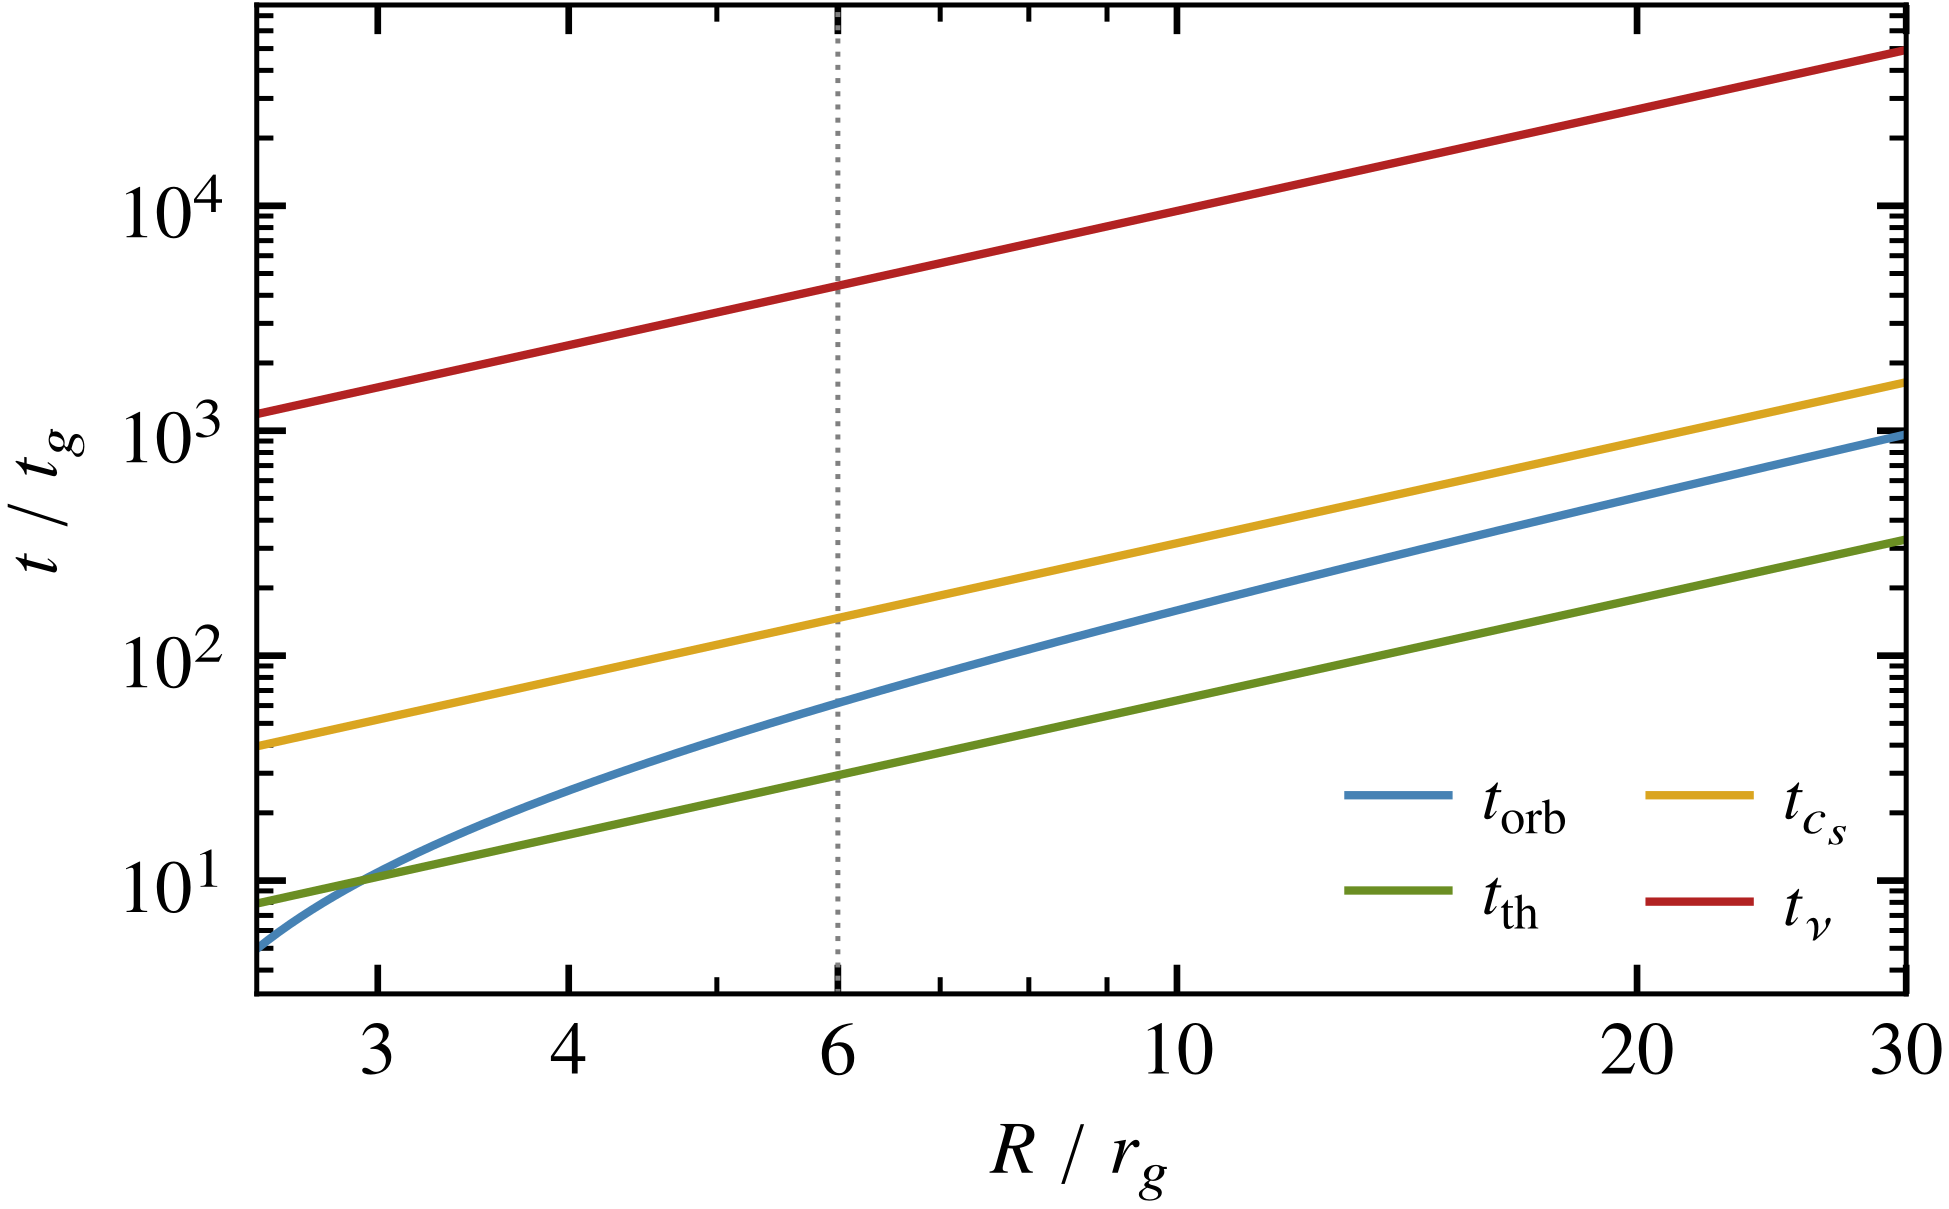
\includegraphics[width=\columnwidth, draft=false]{plots/timescales_col.png}
		\caption{Orbital, thermal, sound crossing and viscous times of the initial disk.}
		\label{fig:timescales}
	\end{figure}

	\begin{figure}[H]
		\centering
		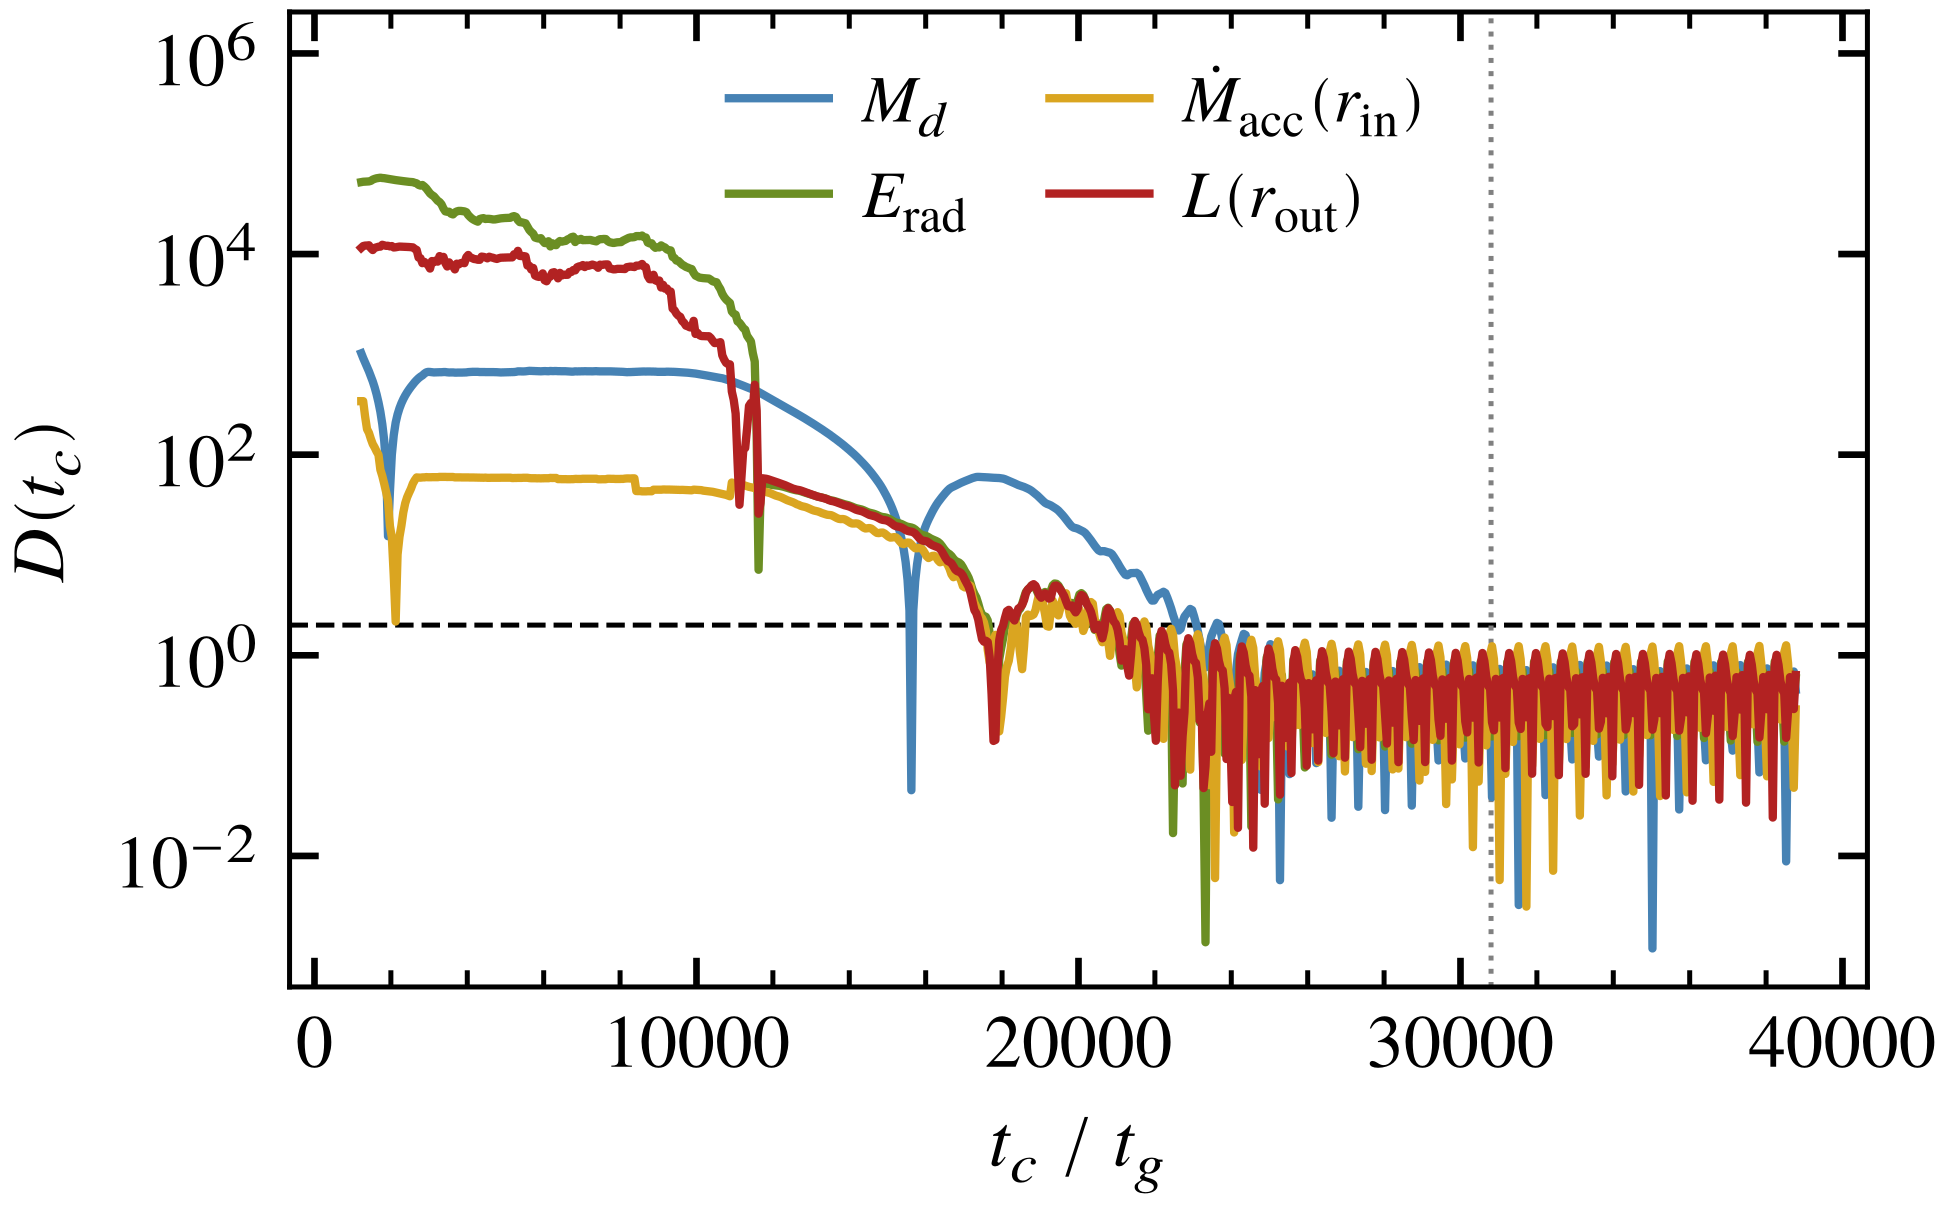
\includegraphics[width=\columnwidth, draft=false]{plots/relax_distance_col.png}
		\caption{Relaxation statistic of the four global quantities of HR. The dashed line marks the threshold and the dotted line
				 the start of the reference period.}
		\label{fig:relax_distance}
	\end{figure}

	\begin{figure}[H]
		\centering
		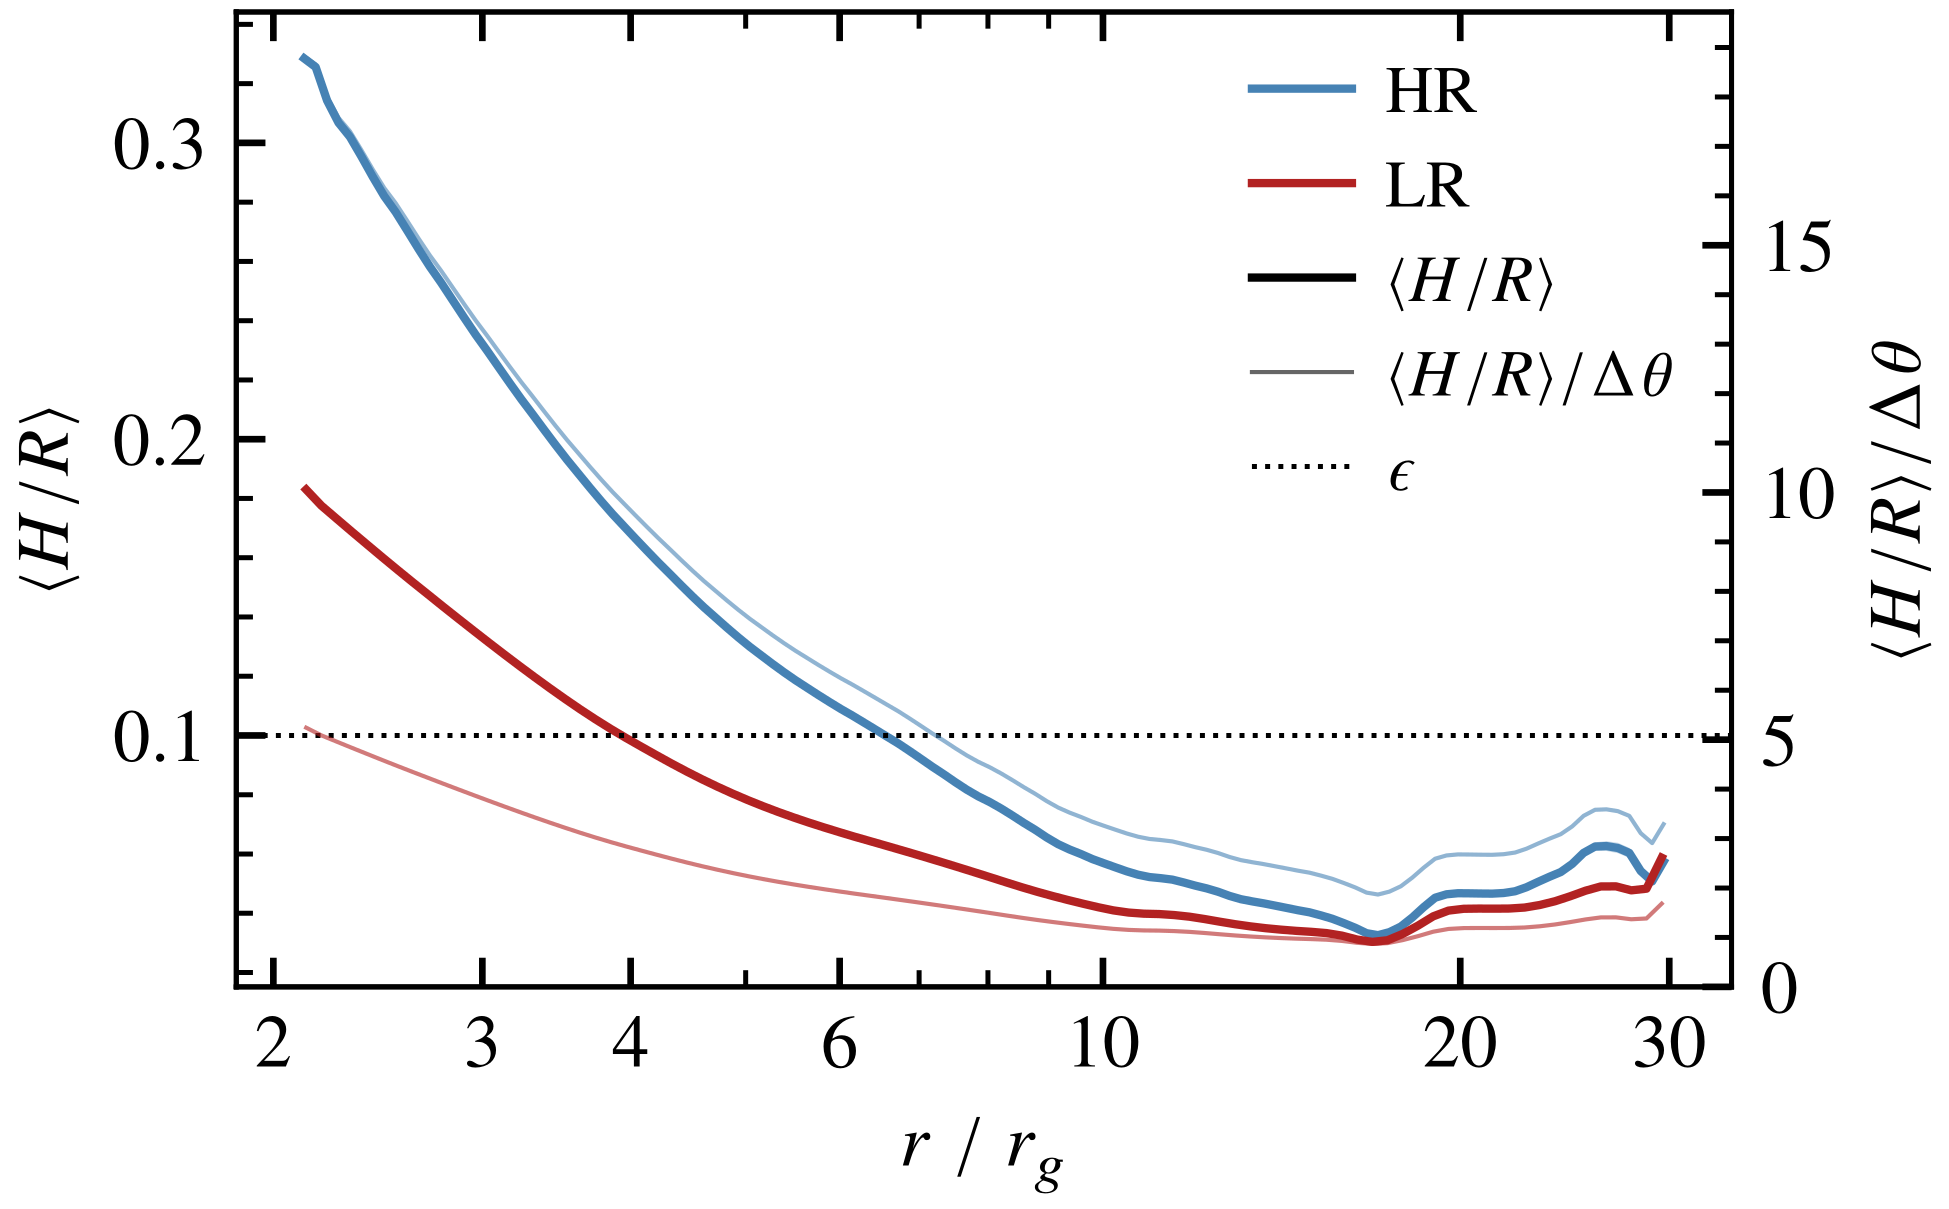
\includegraphics[width=\columnwidth, draft=false]{plots/aspect_col.png}
		\caption{Time averaged aspect ratio of the disk and its resolution in cells per scale height.}
		\label{fig:aspect}
	\end{figure}

	\begin{figure}[H]
		\centering
		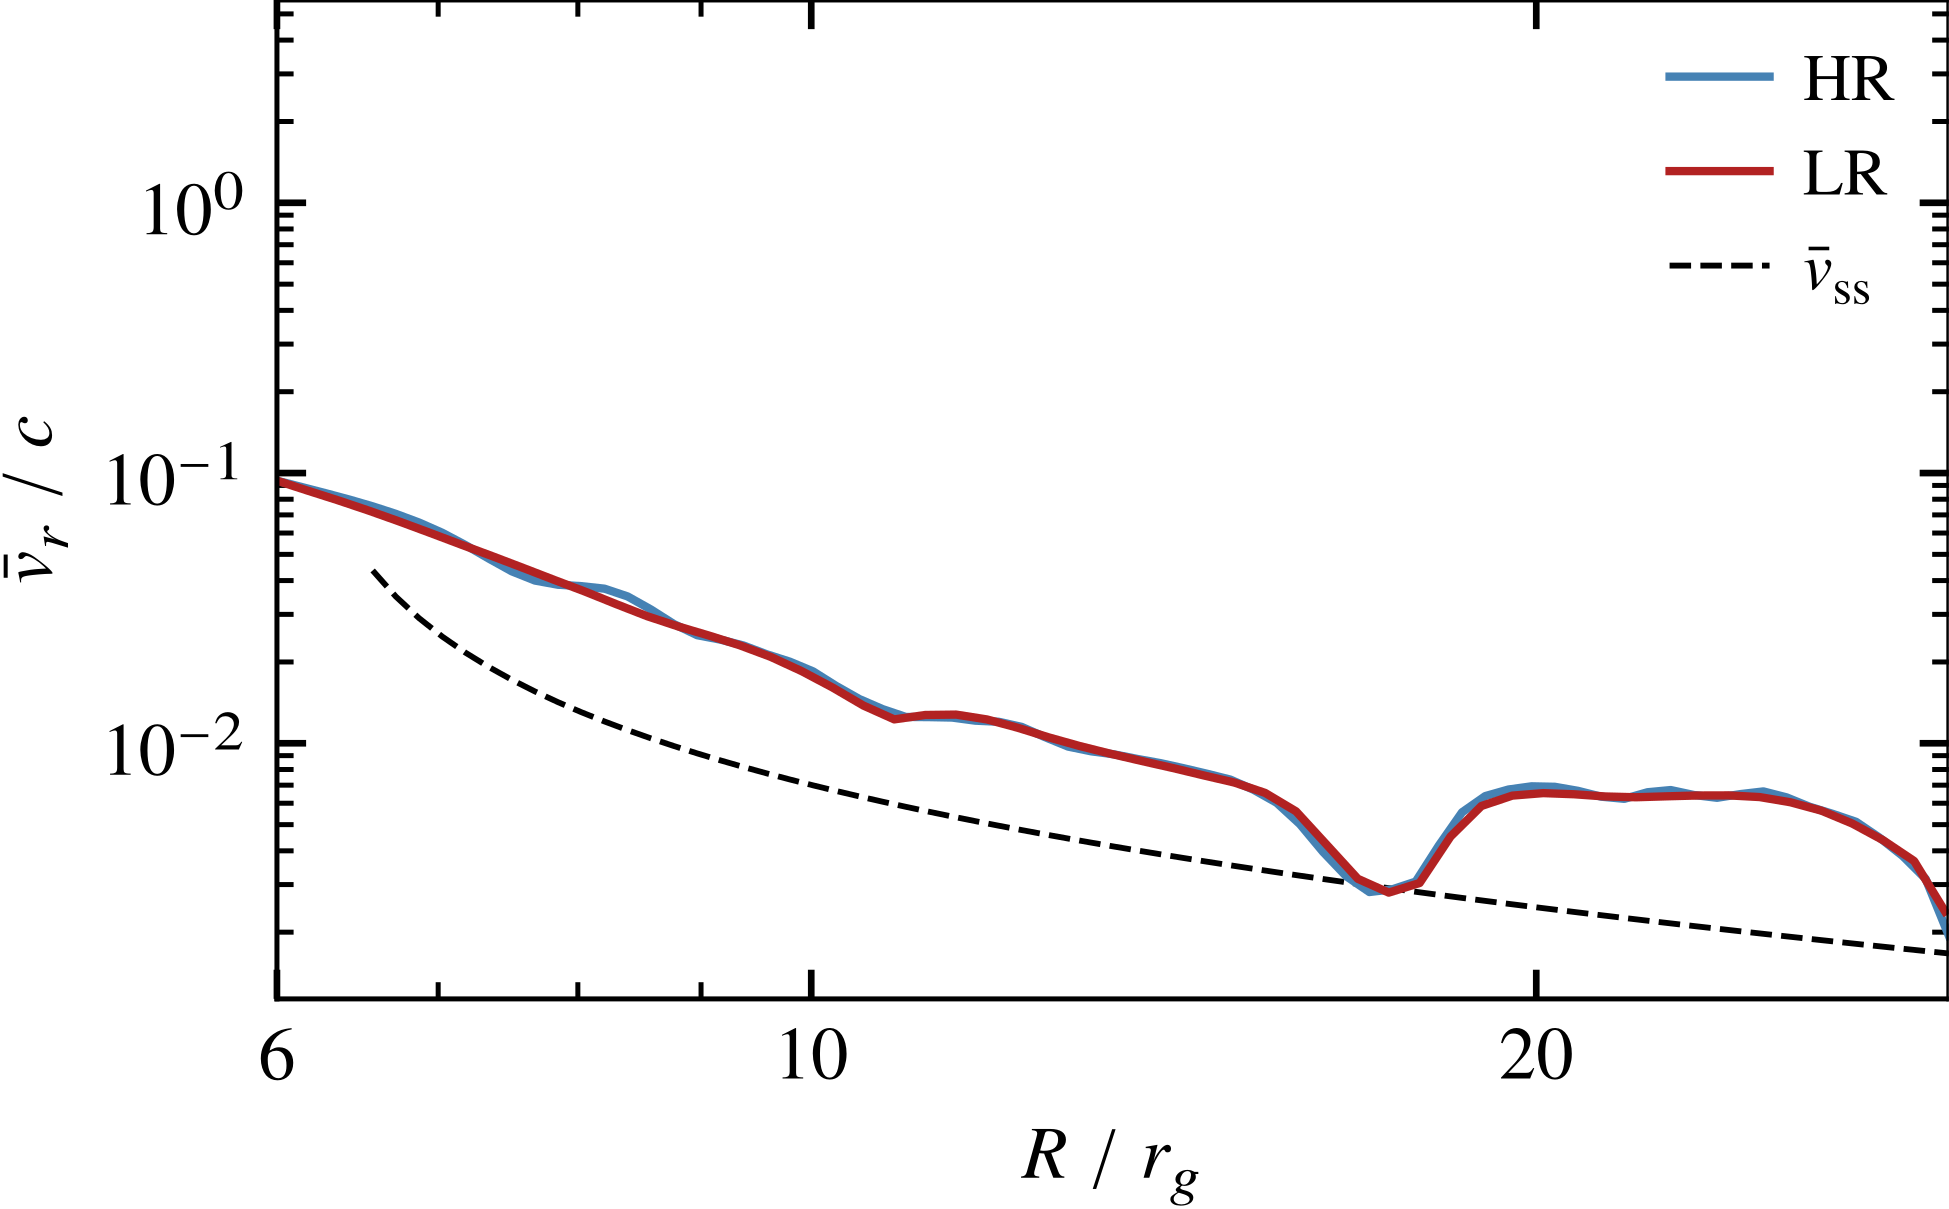
\includegraphics[width=\columnwidth, draft=false]{plots/inflow_col.png}
		\caption{Mean radial inflow speed from accretion rate and surface density, compared with the steady state value of the
				 prescribed viscosity.}
		\label{fig:inflow}
	\end{figure}

	\begin{figure}[H]
		\centering
		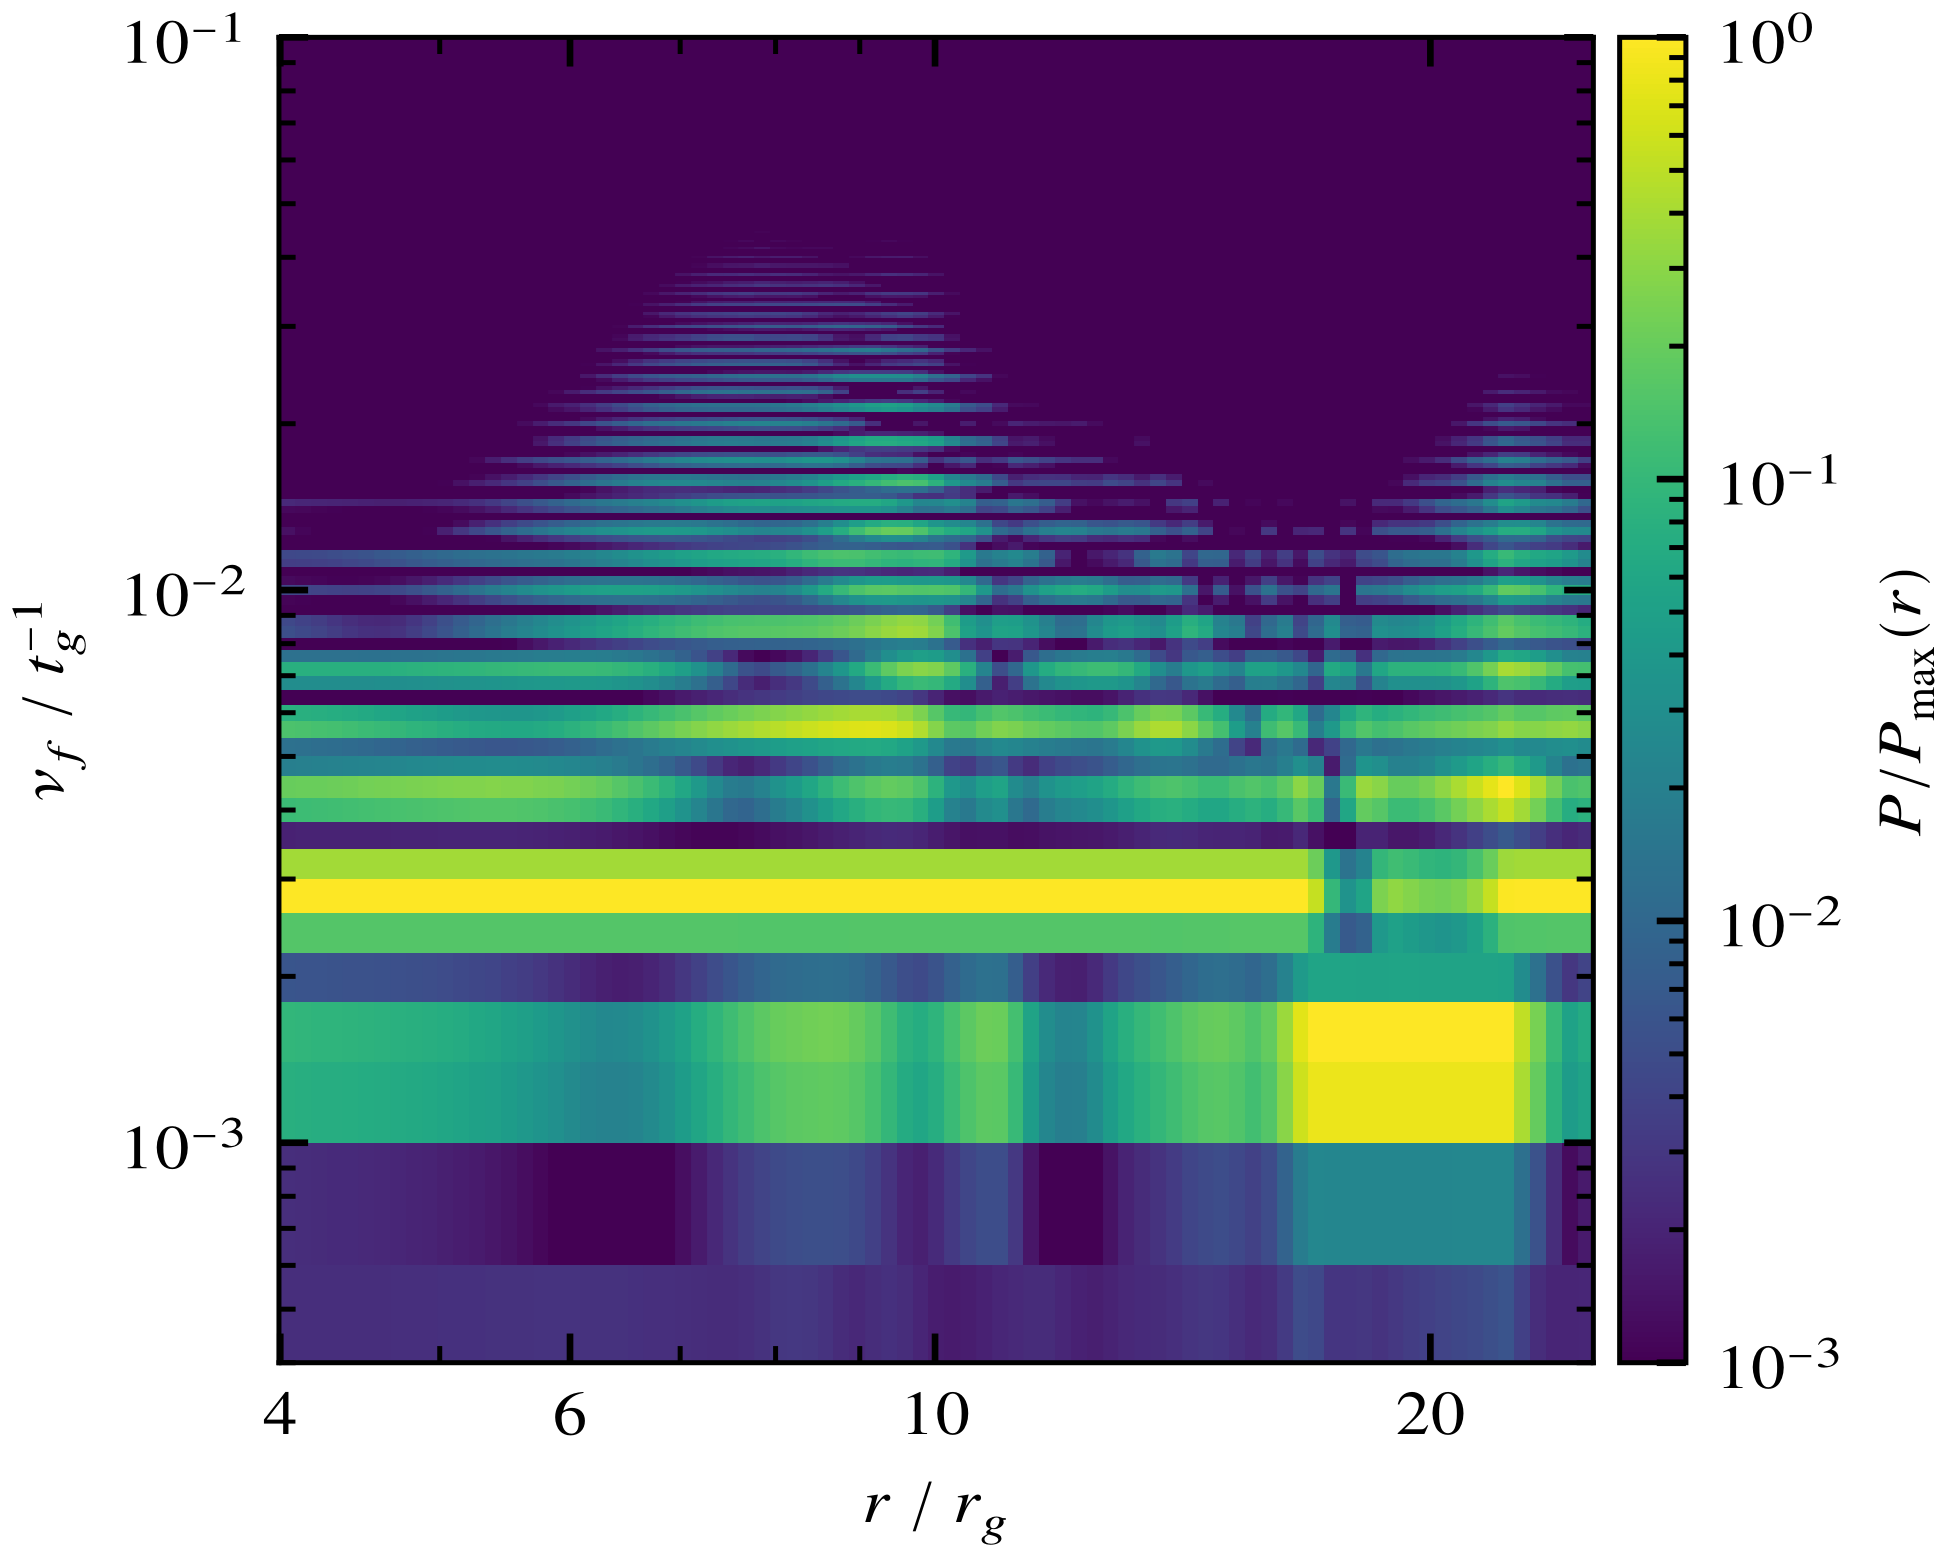
\includegraphics[width=\columnwidth, draft=false]{plots/wave_spectrum_col.png}
		\caption{Power spectrum of the surface density perturbation of HR at each radius, normalized to its maximum.}
		\label{fig:wave_spectrum}
	\end{figure}

	\begin{figure*}[p]
		\centering
		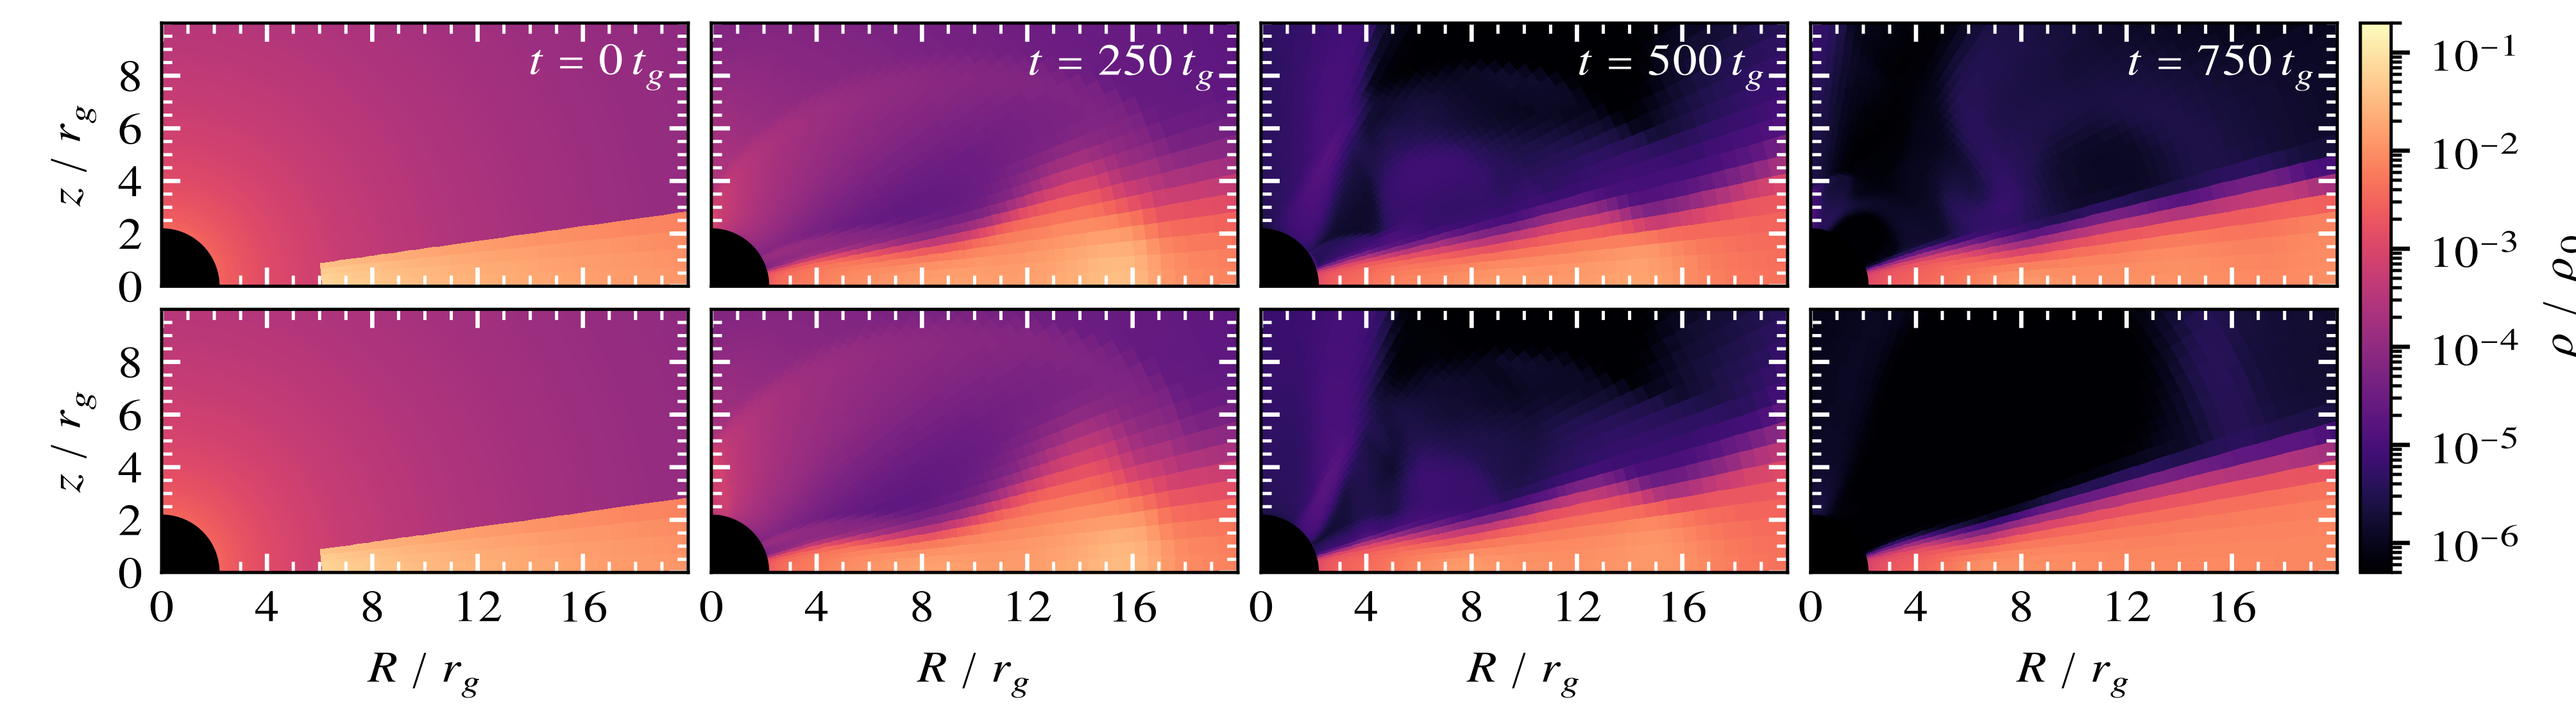
\includegraphics[width=\textwidth, draft=false]{plots/valid_mhd_rho_text.png}
		\vspace{0.5\baselineskip}
		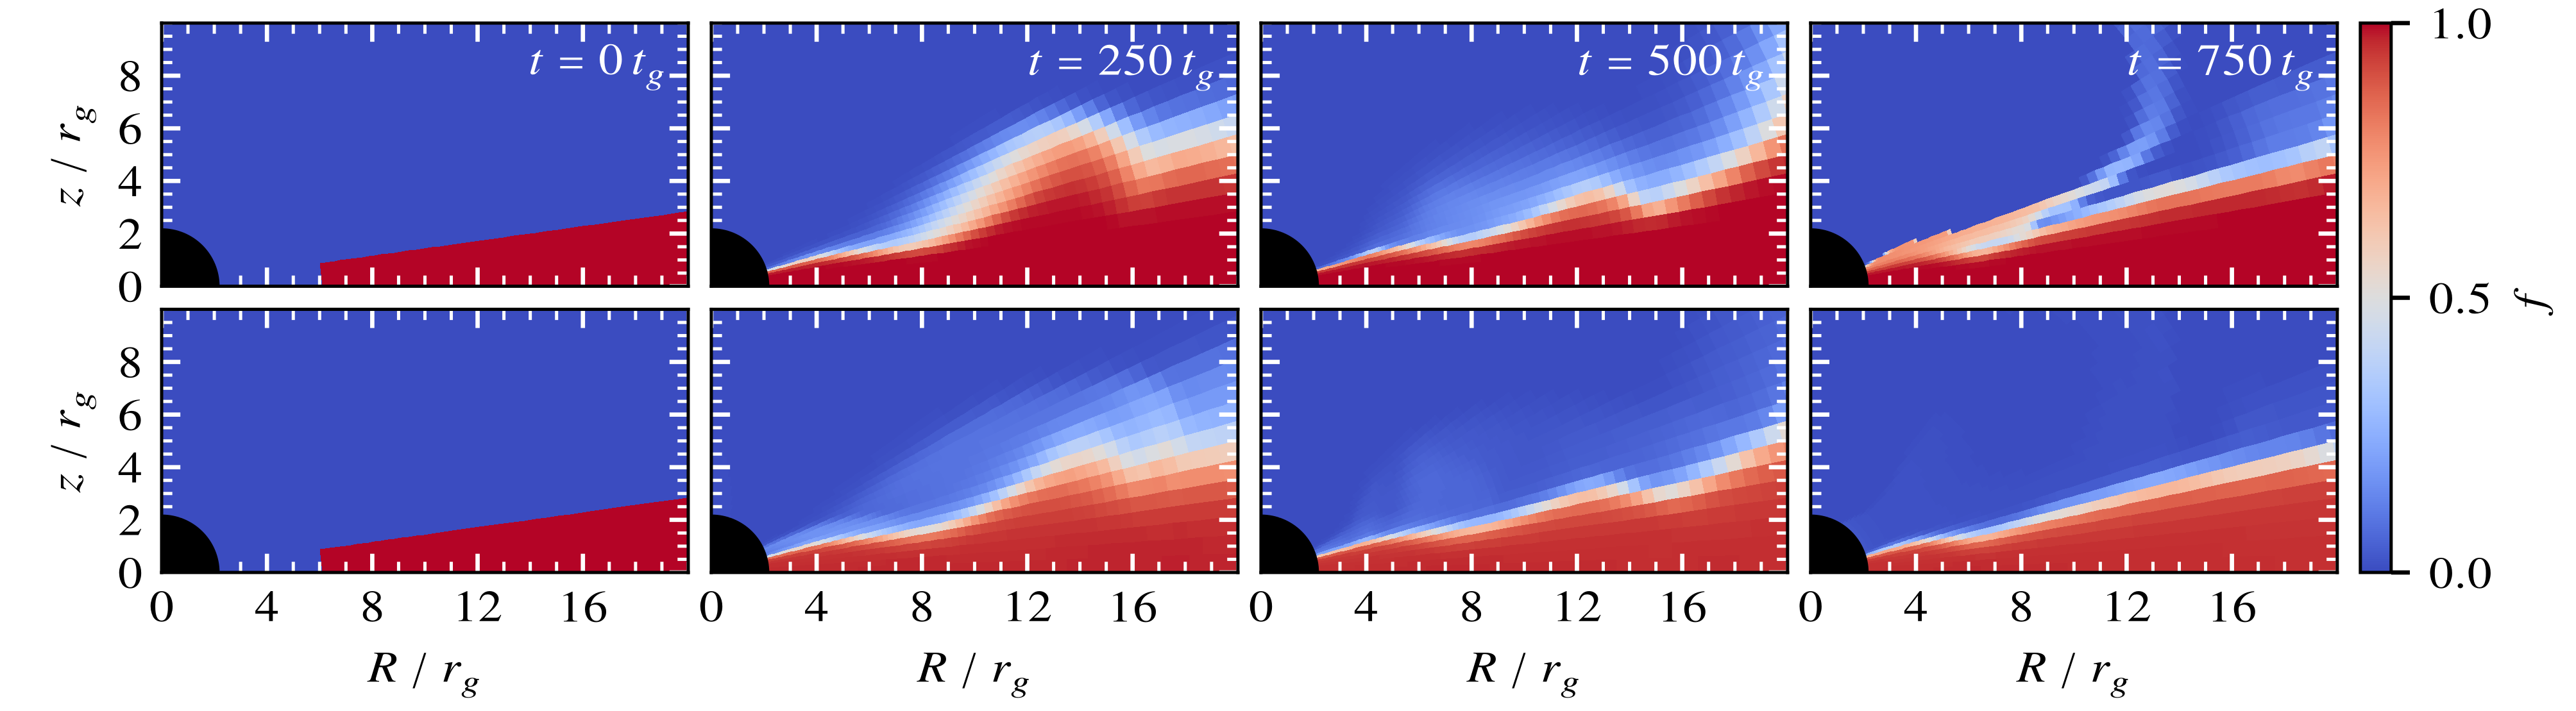
\includegraphics[width=\textwidth, draft=false]{plots/valid_mhd_class_text.png}
		\vspace{0.5\baselineskip}
		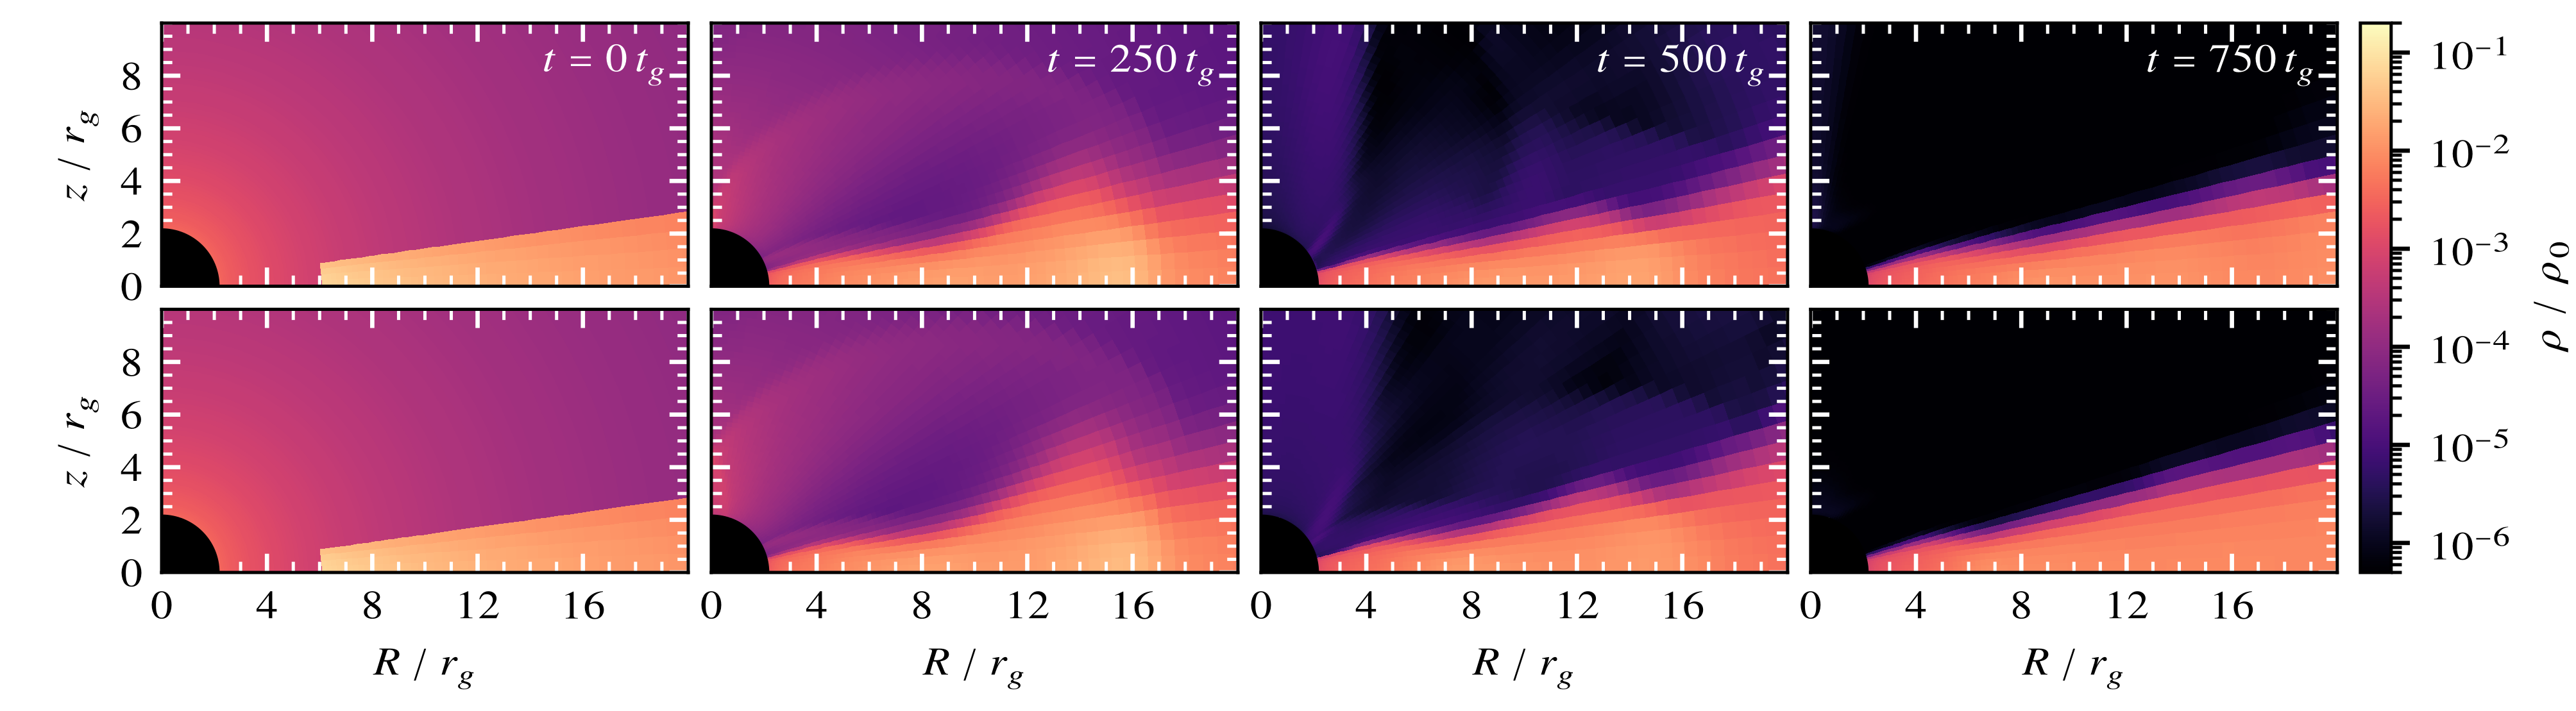
\includegraphics[width=\textwidth, draft=false]{plots/valid_rmhd_rho_text.png}
		\vspace{0.5\baselineskip}
		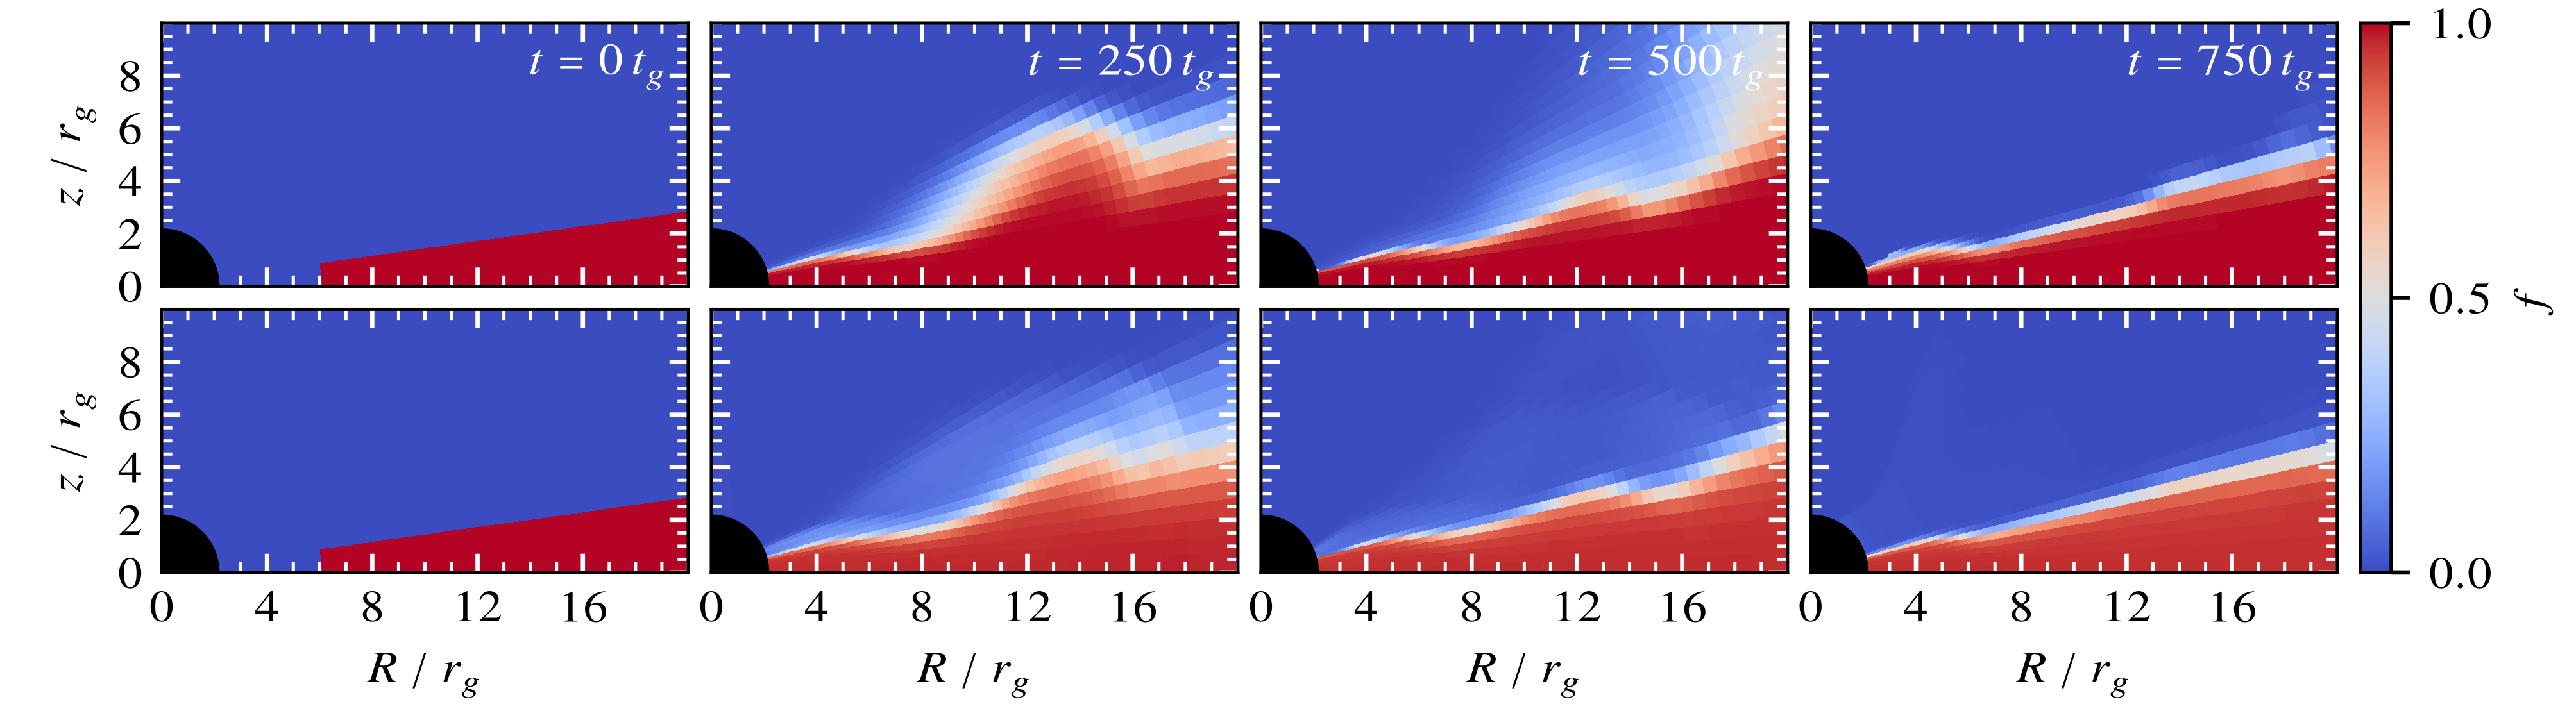
\includegraphics[width=\textwidth, draft=false]{plots/valid_rmhd_class_text.png}
		\caption{Validation for the magnetohydrodynamic \textit{(upper two)} and resistive magnetohydrodynamic \textit{(lower two)}
				 cases, arranged as in \Cref{fig:valid_rho,fig:valid_class}.}
		\label{fig:valid_mhd}
	\end{figure*}

	\begin{figure*}[p]
		\centering
		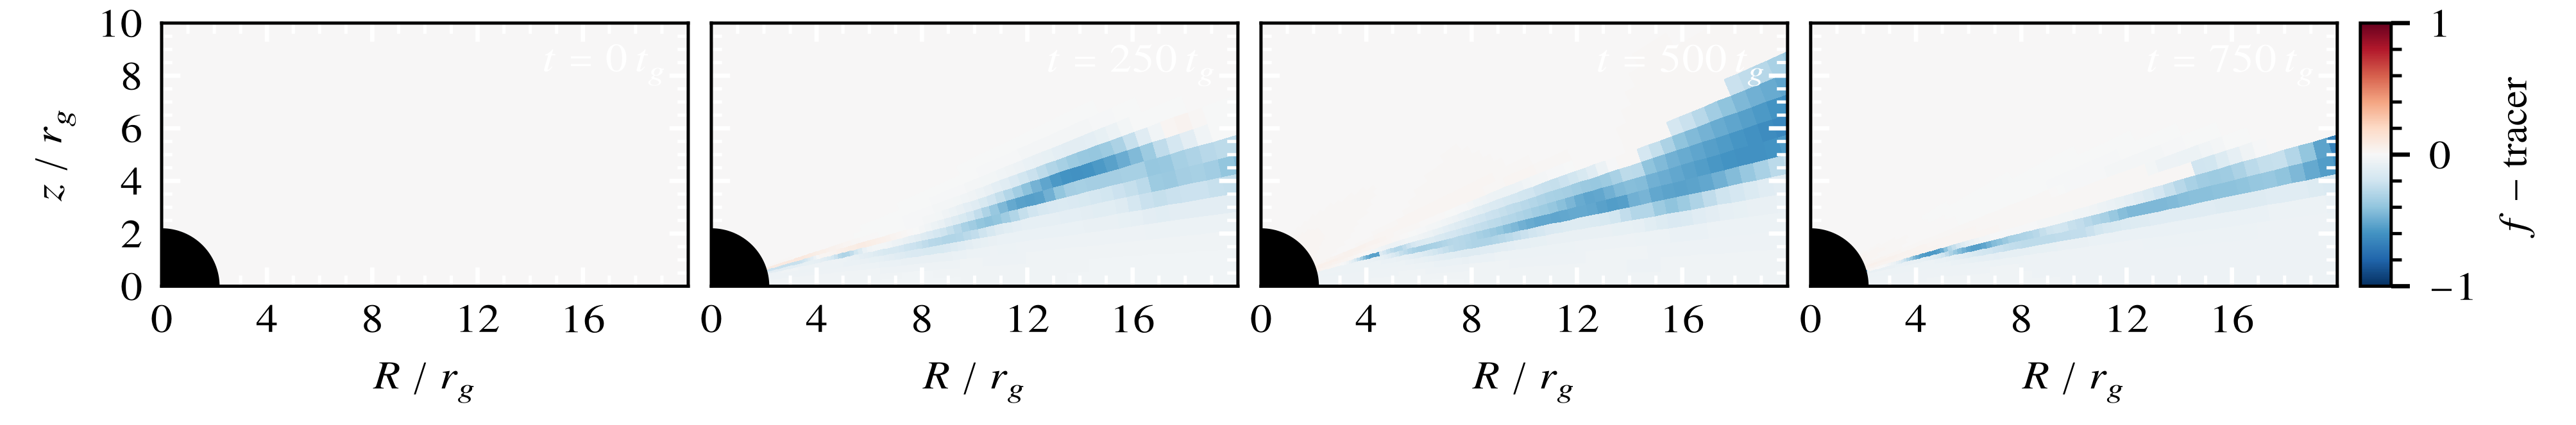
\includegraphics[width=\textwidth, draft=false]{plots/valid_hd_diff_text.png}
		\vspace{0.5\baselineskip}
		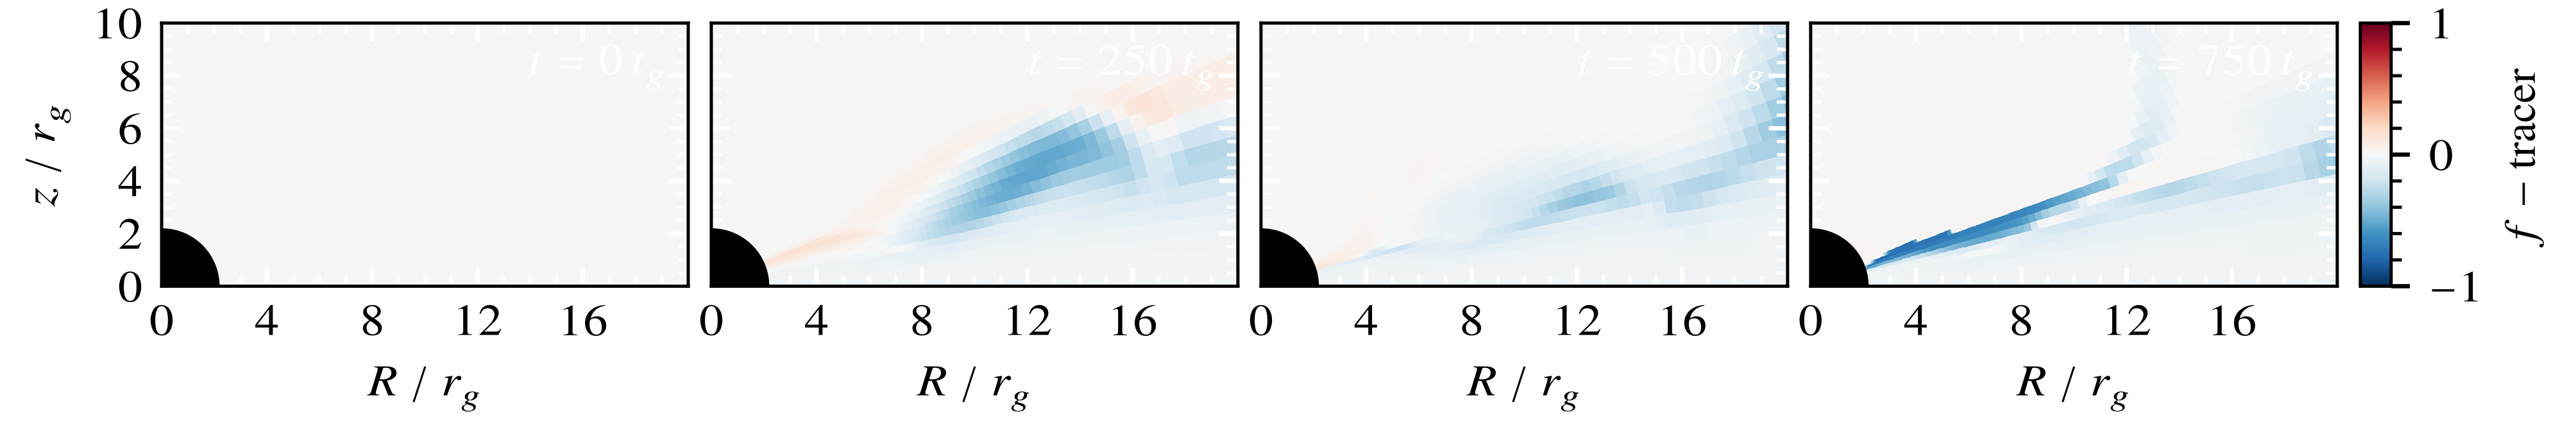
\includegraphics[width=\textwidth, draft=false]{plots/valid_mhd_diff_text.png}
		\vspace{0.5\baselineskip}
		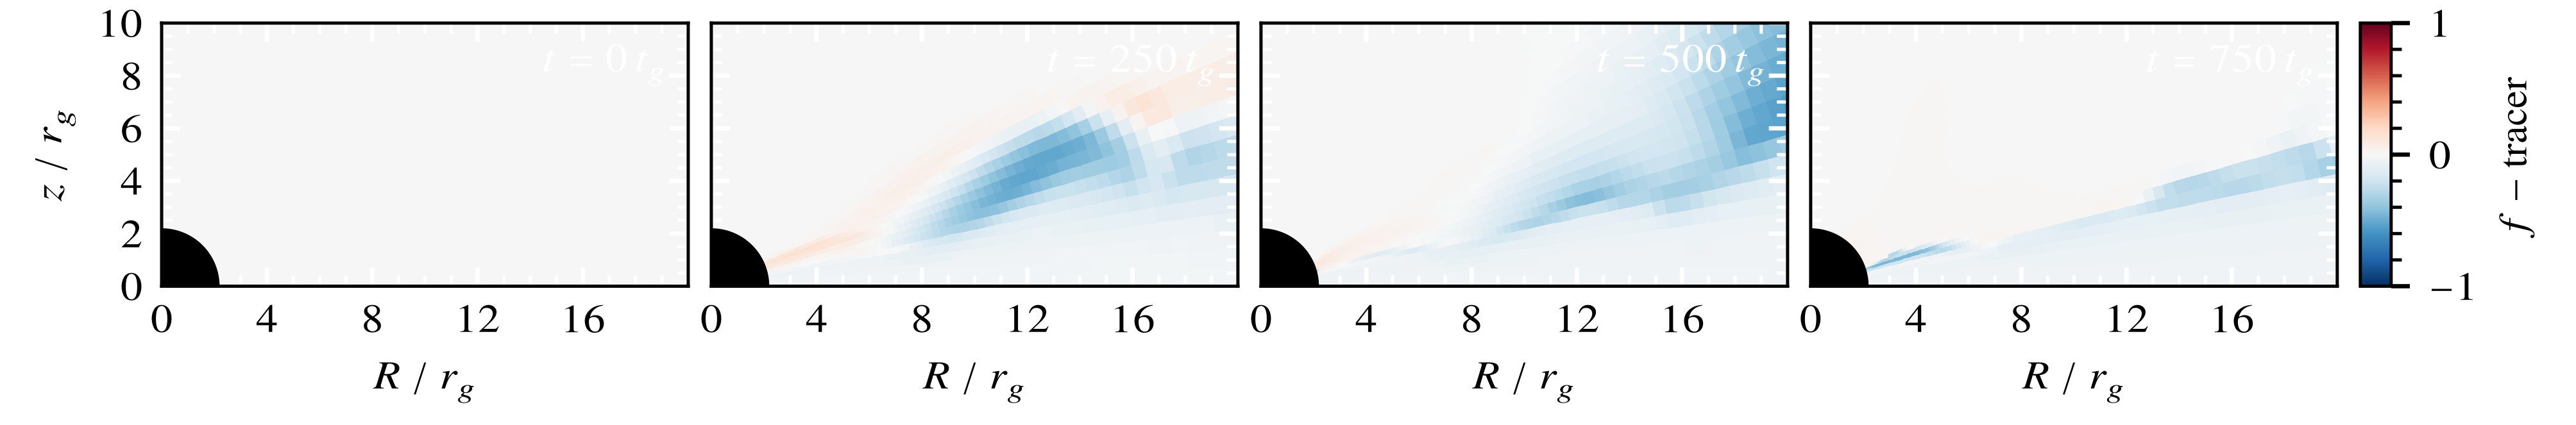
\includegraphics[width=\textwidth, draft=false]{plots/valid_rmhd_diff_text.png}
		\caption{Difference between DiskFraction and tracer in the classifier driven hydrodynamic, magnetohydrodynamic and resistive
				 runs \textit{(top to bottom)}.}
		\label{fig:valid_diff}
	\end{figure*}

	\begin{figure*}[p]
		\centering
		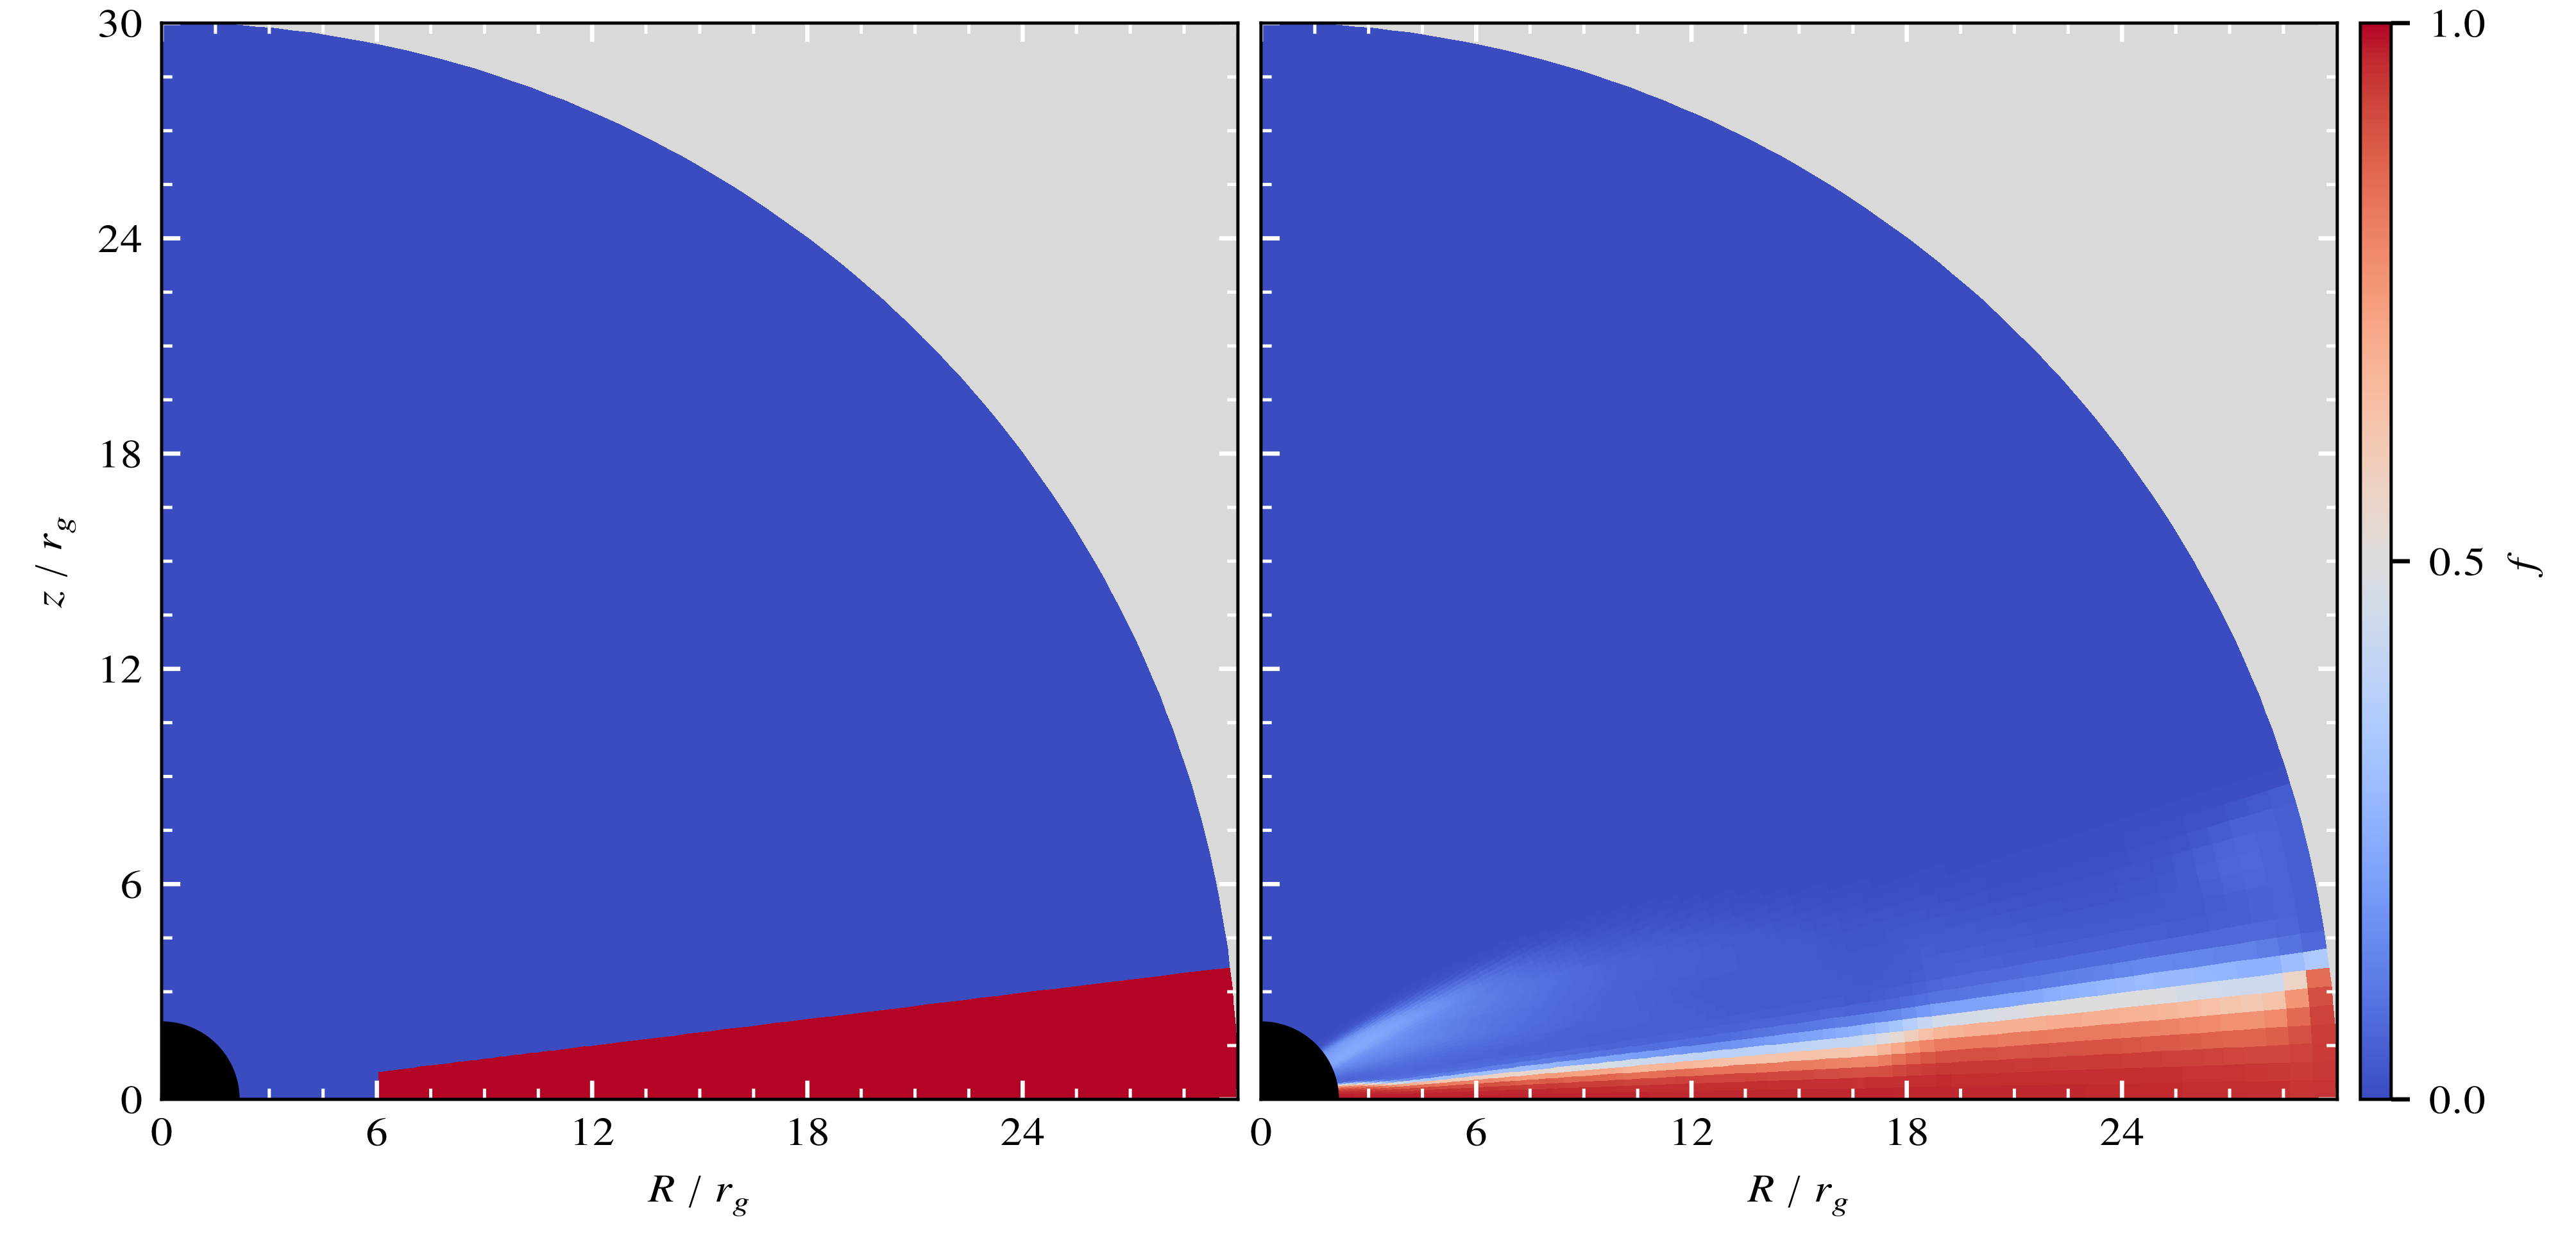
\includegraphics[width=\textwidth, draft=false]{plots/domain_f_text.png}
		\vspace{0.5\baselineskip}
		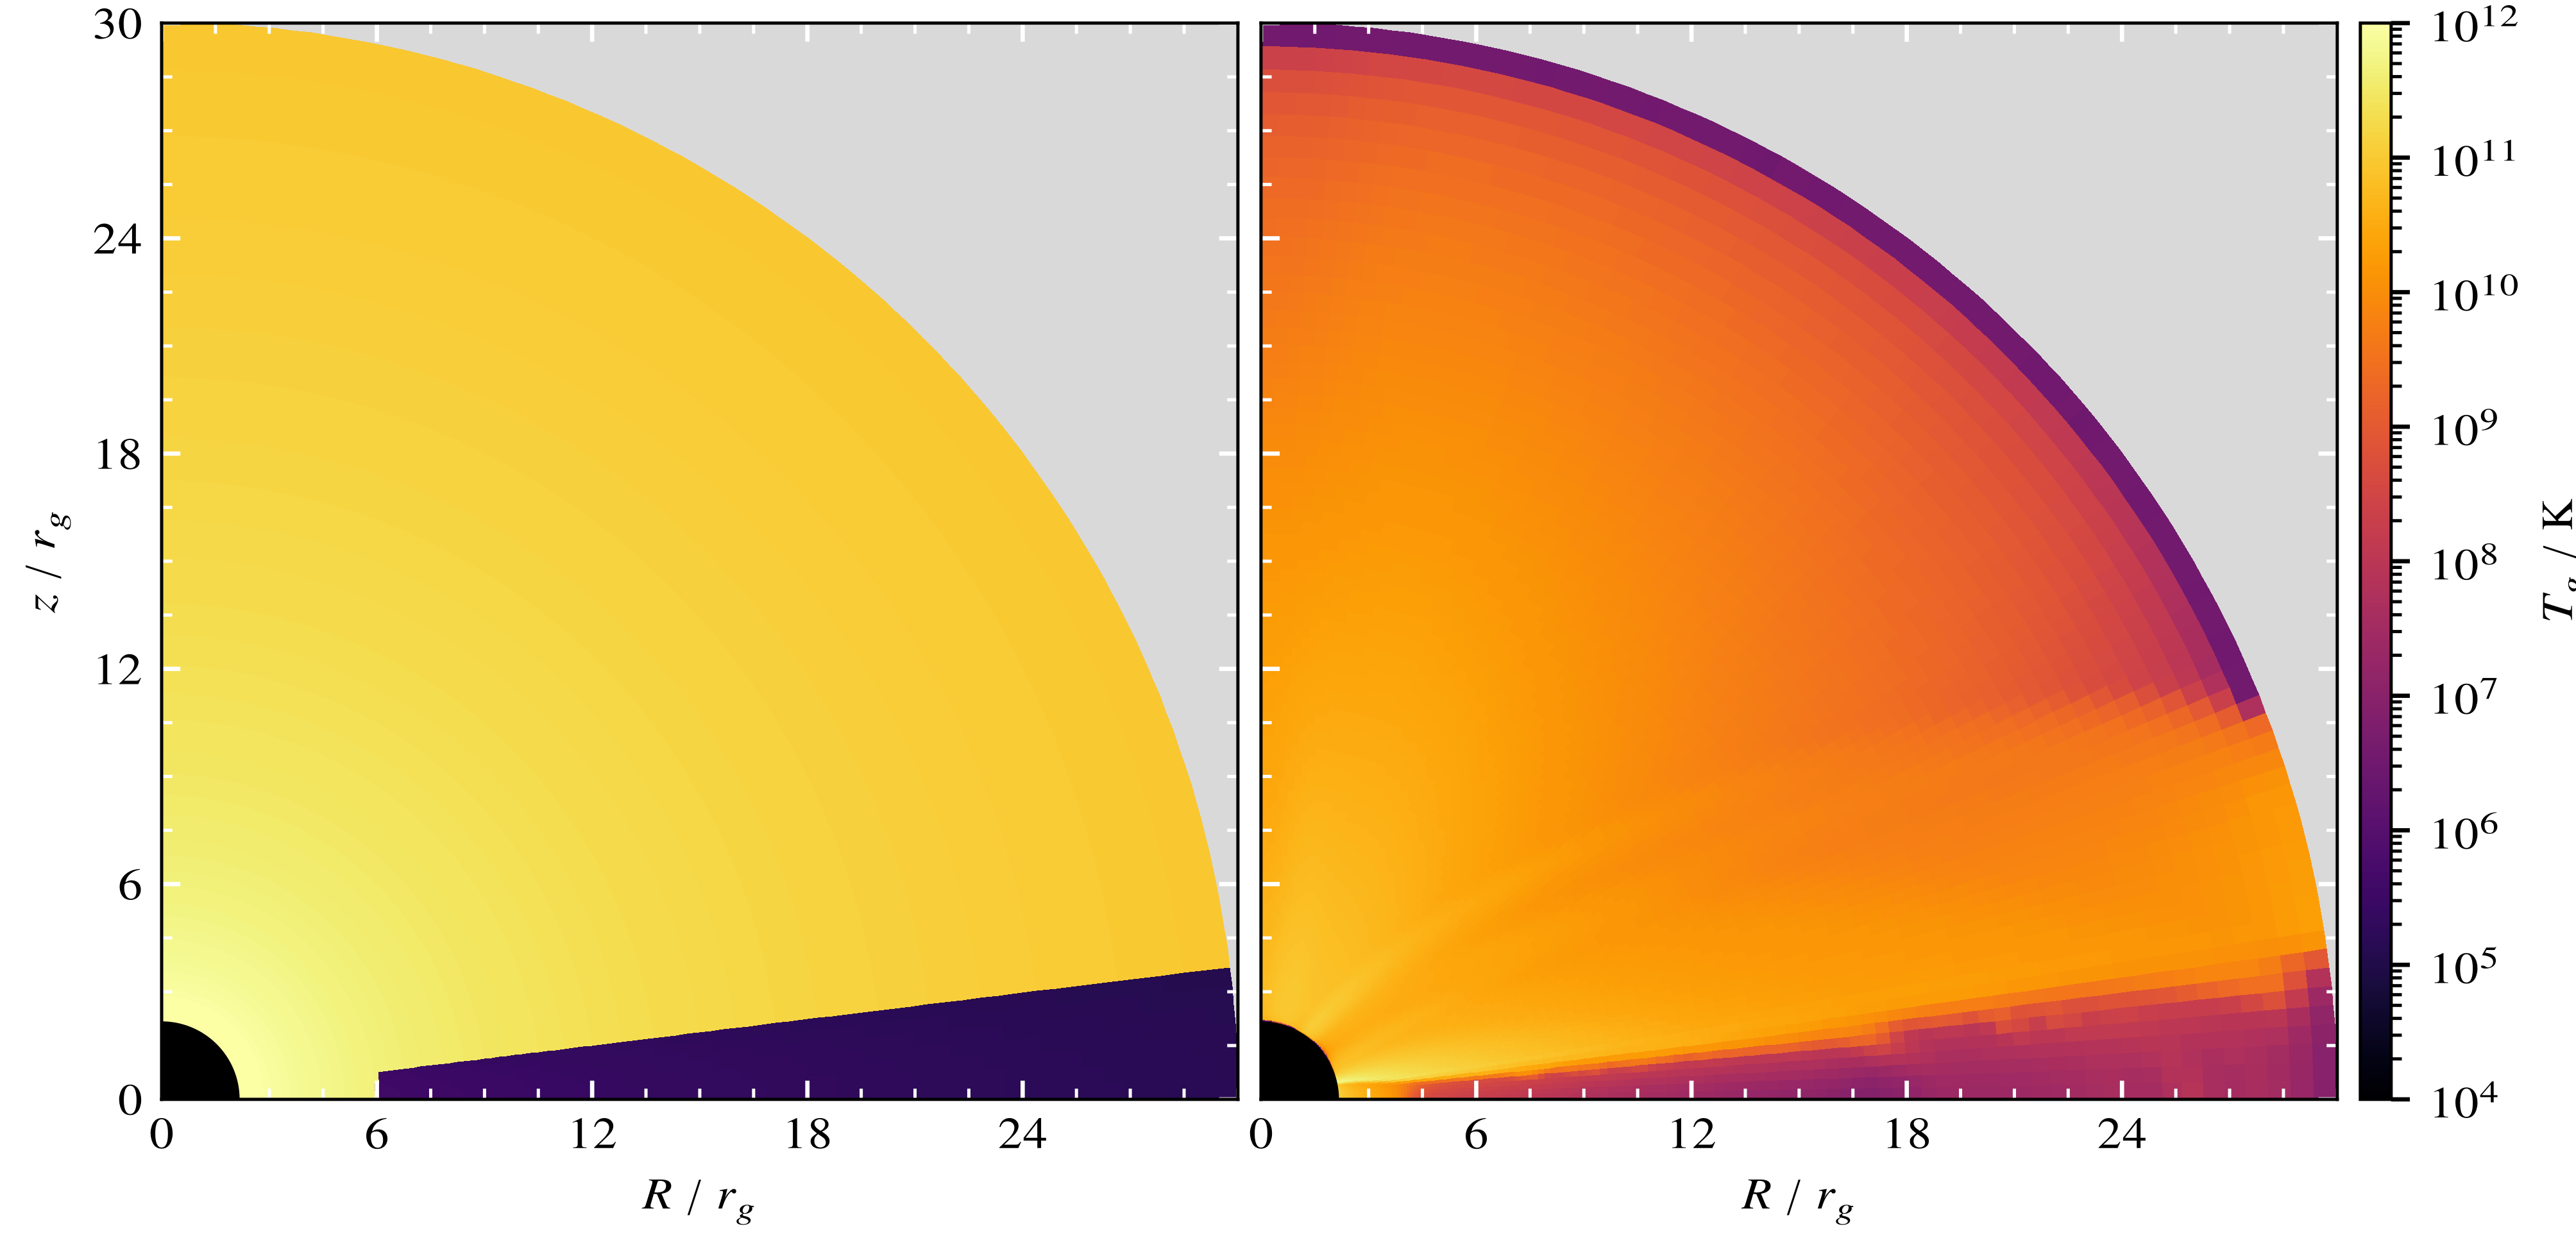
\includegraphics[width=\textwidth, draft=false]{plots/domain_Tg_text.png}
		\caption{DiskFraction \textit{(top)} and gas temperature \textit{(bottom)} of HR initially \textit{(left)} and averaged over the
				 last \num{10000} gravitational times \textit{(right)}.}
		\label{fig:domain_f_Tg}
	\end{figure*}

	\begin{figure*}[p]
		\centering
		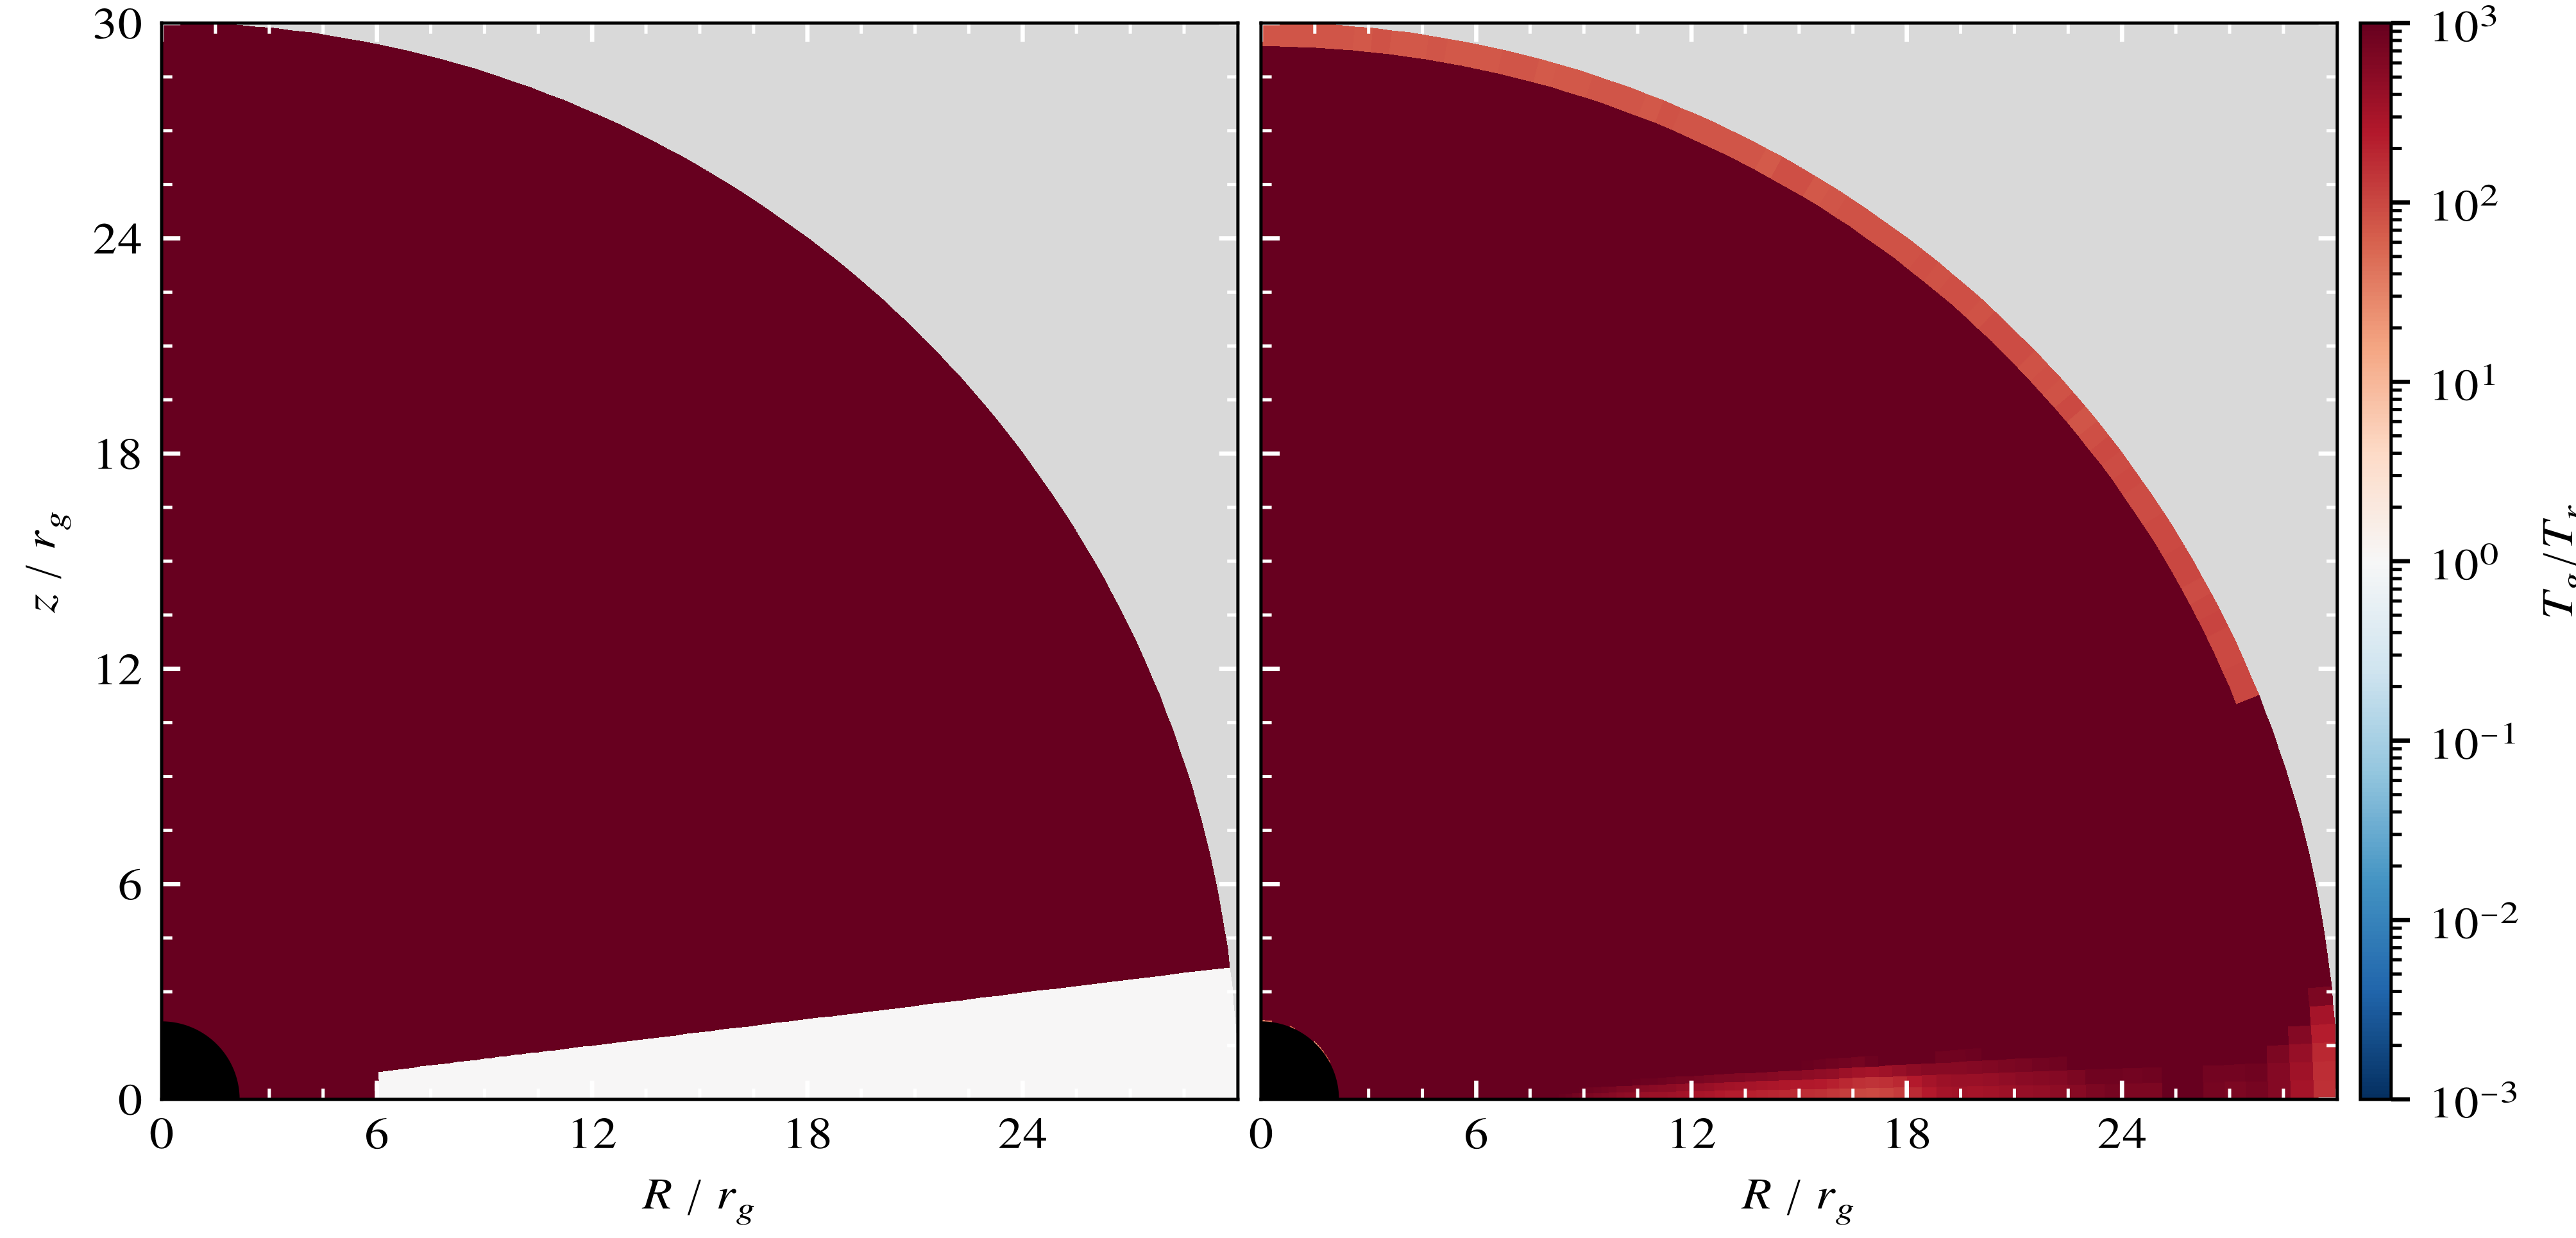
\includegraphics[width=\textwidth, draft=false]{plots/domain_ratio_text.png}
		\vspace{0.5\baselineskip}
		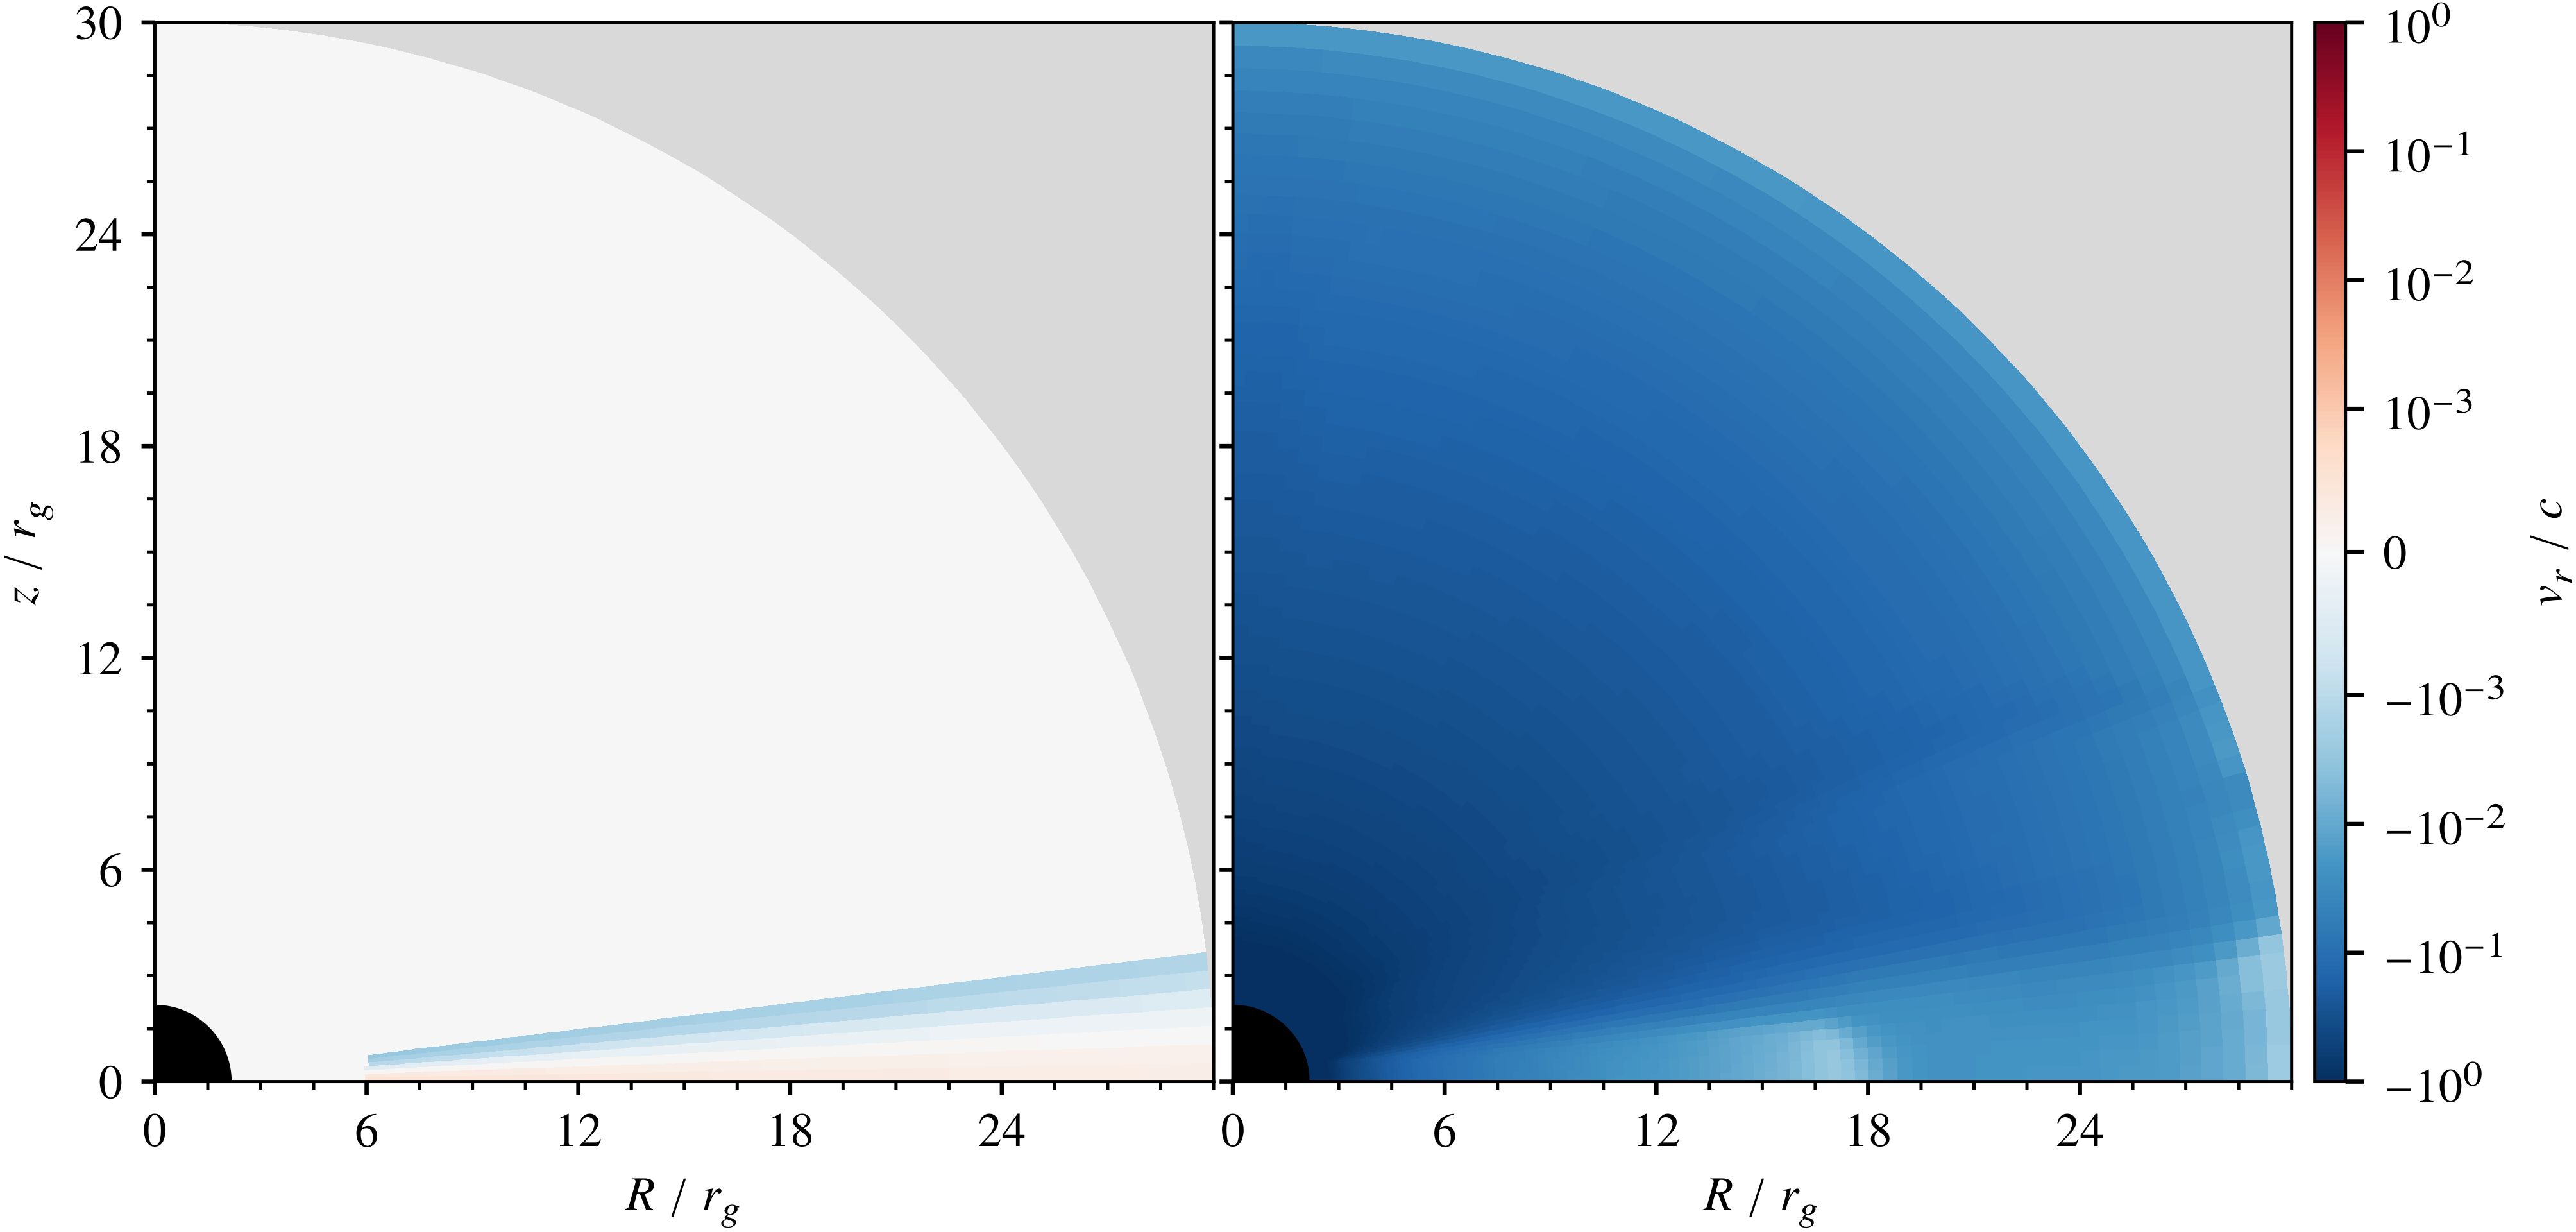
\includegraphics[width=\textwidth, draft=false]{plots/domain_vr_text.png}
		\caption{Ratio of gas to radiation temperature \textit{(top)} and radial velocity \textit{(bottom)} of HR, arranged as in
				 \Cref{fig:domain_f_Tg}.}
		\label{fig:domain_ratio_vr}
	\end{figure*}

	\begin{figure*}[p]
		\centering
		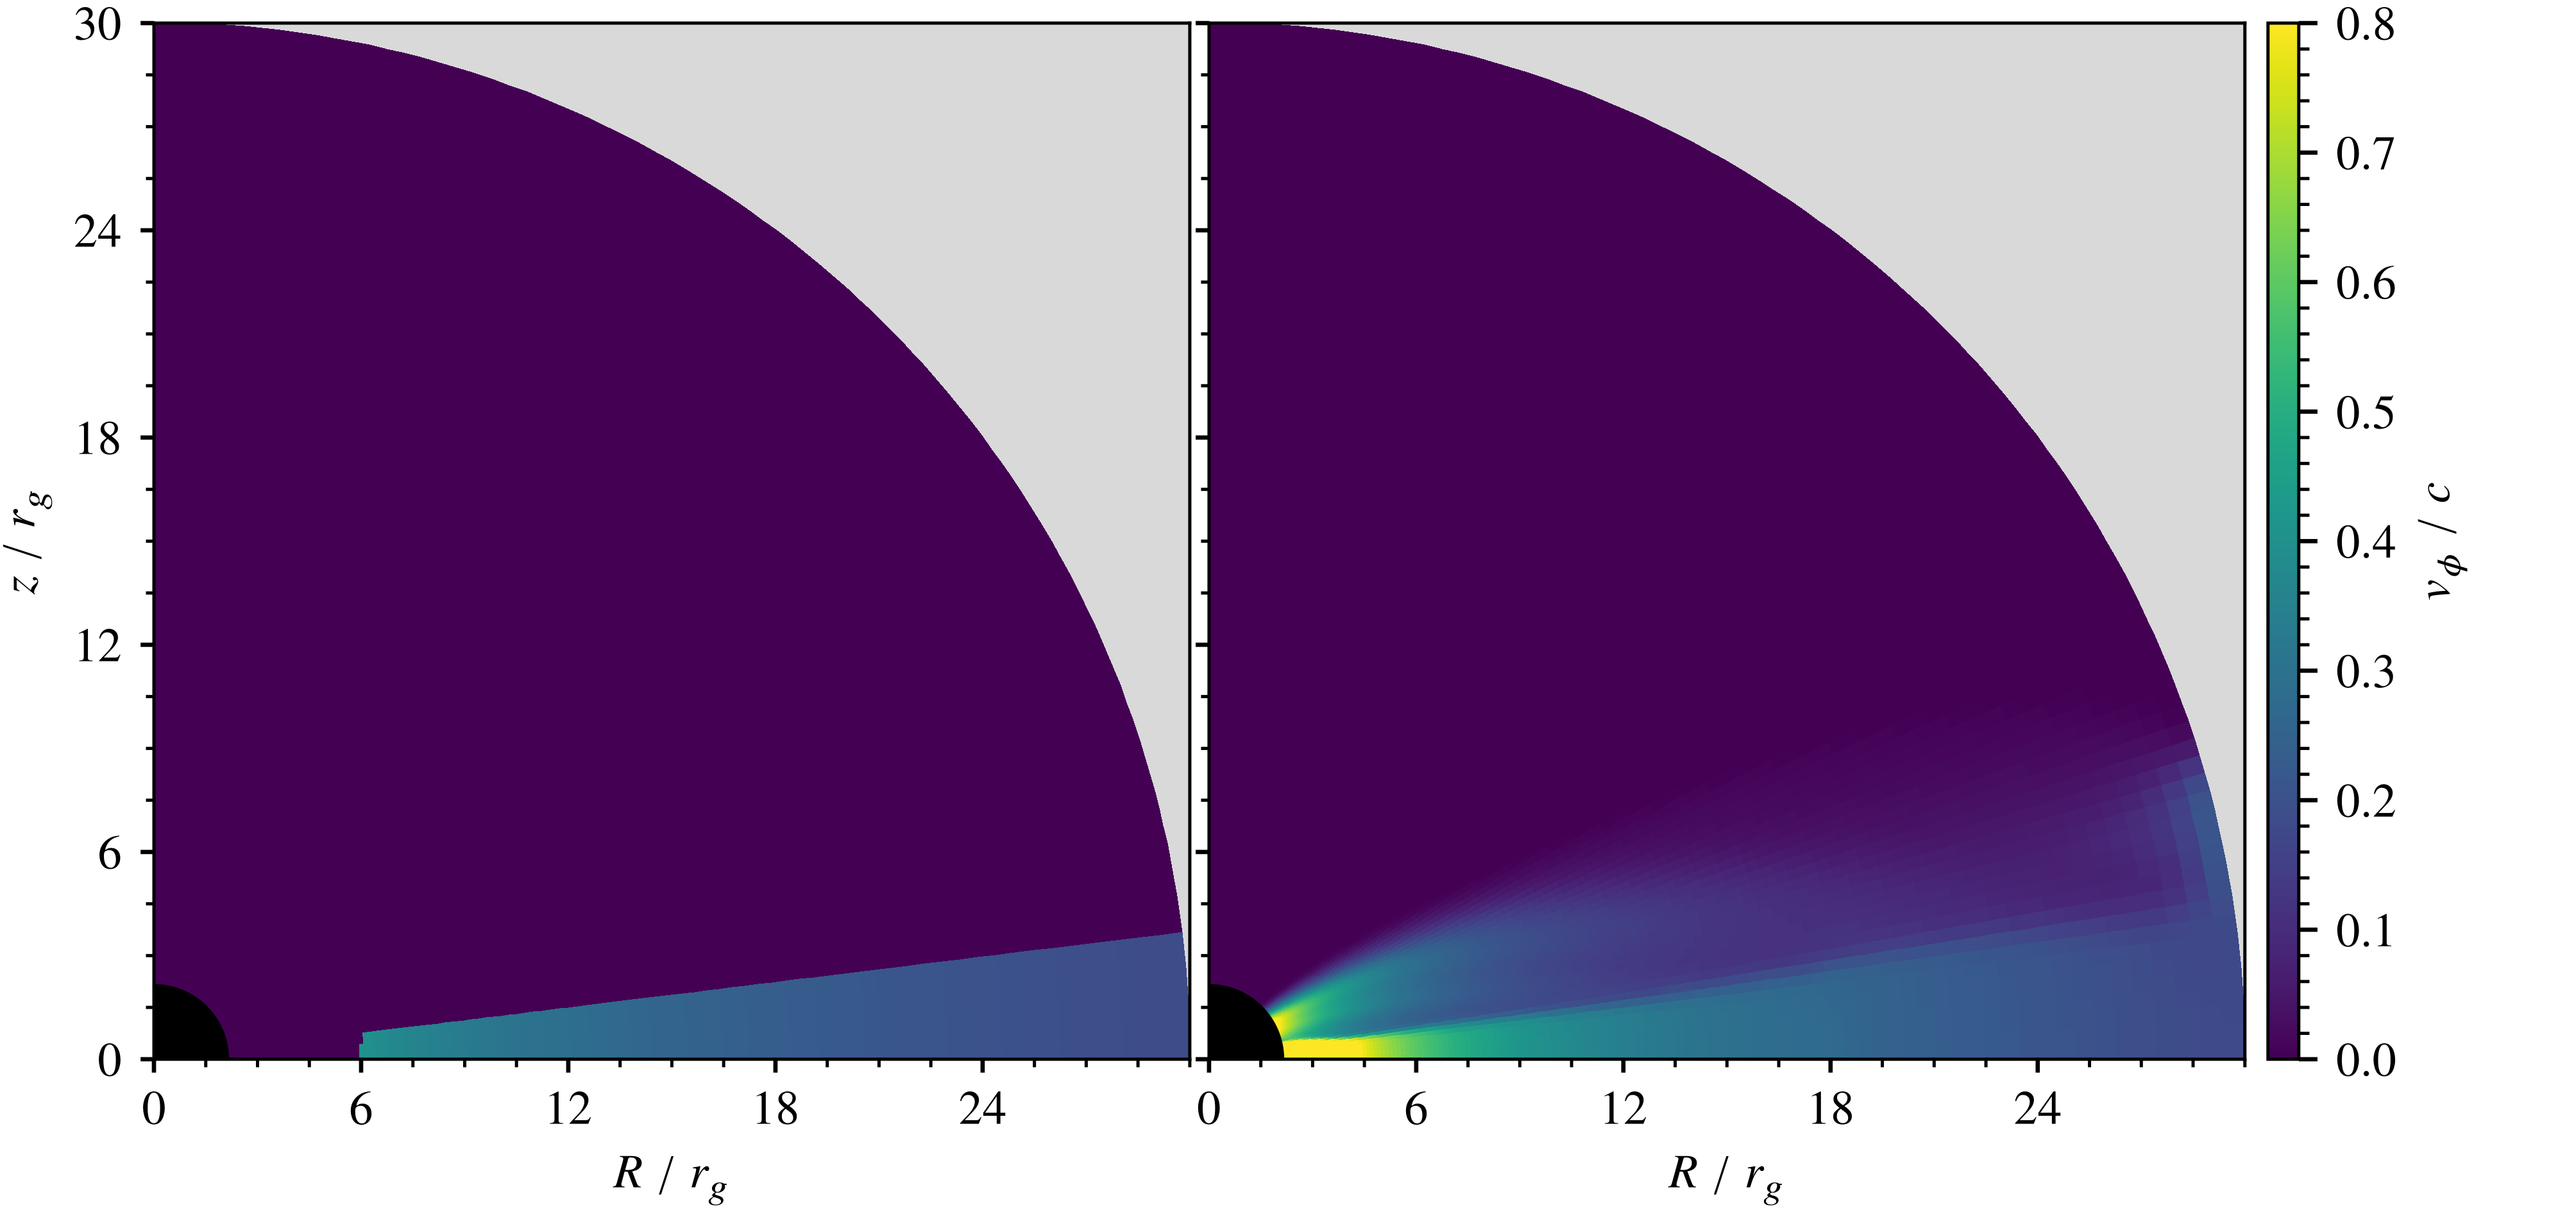
\includegraphics[width=\textwidth, draft=false]{plots/domain_vphi_text.png}
		\vspace{0.5\baselineskip}
		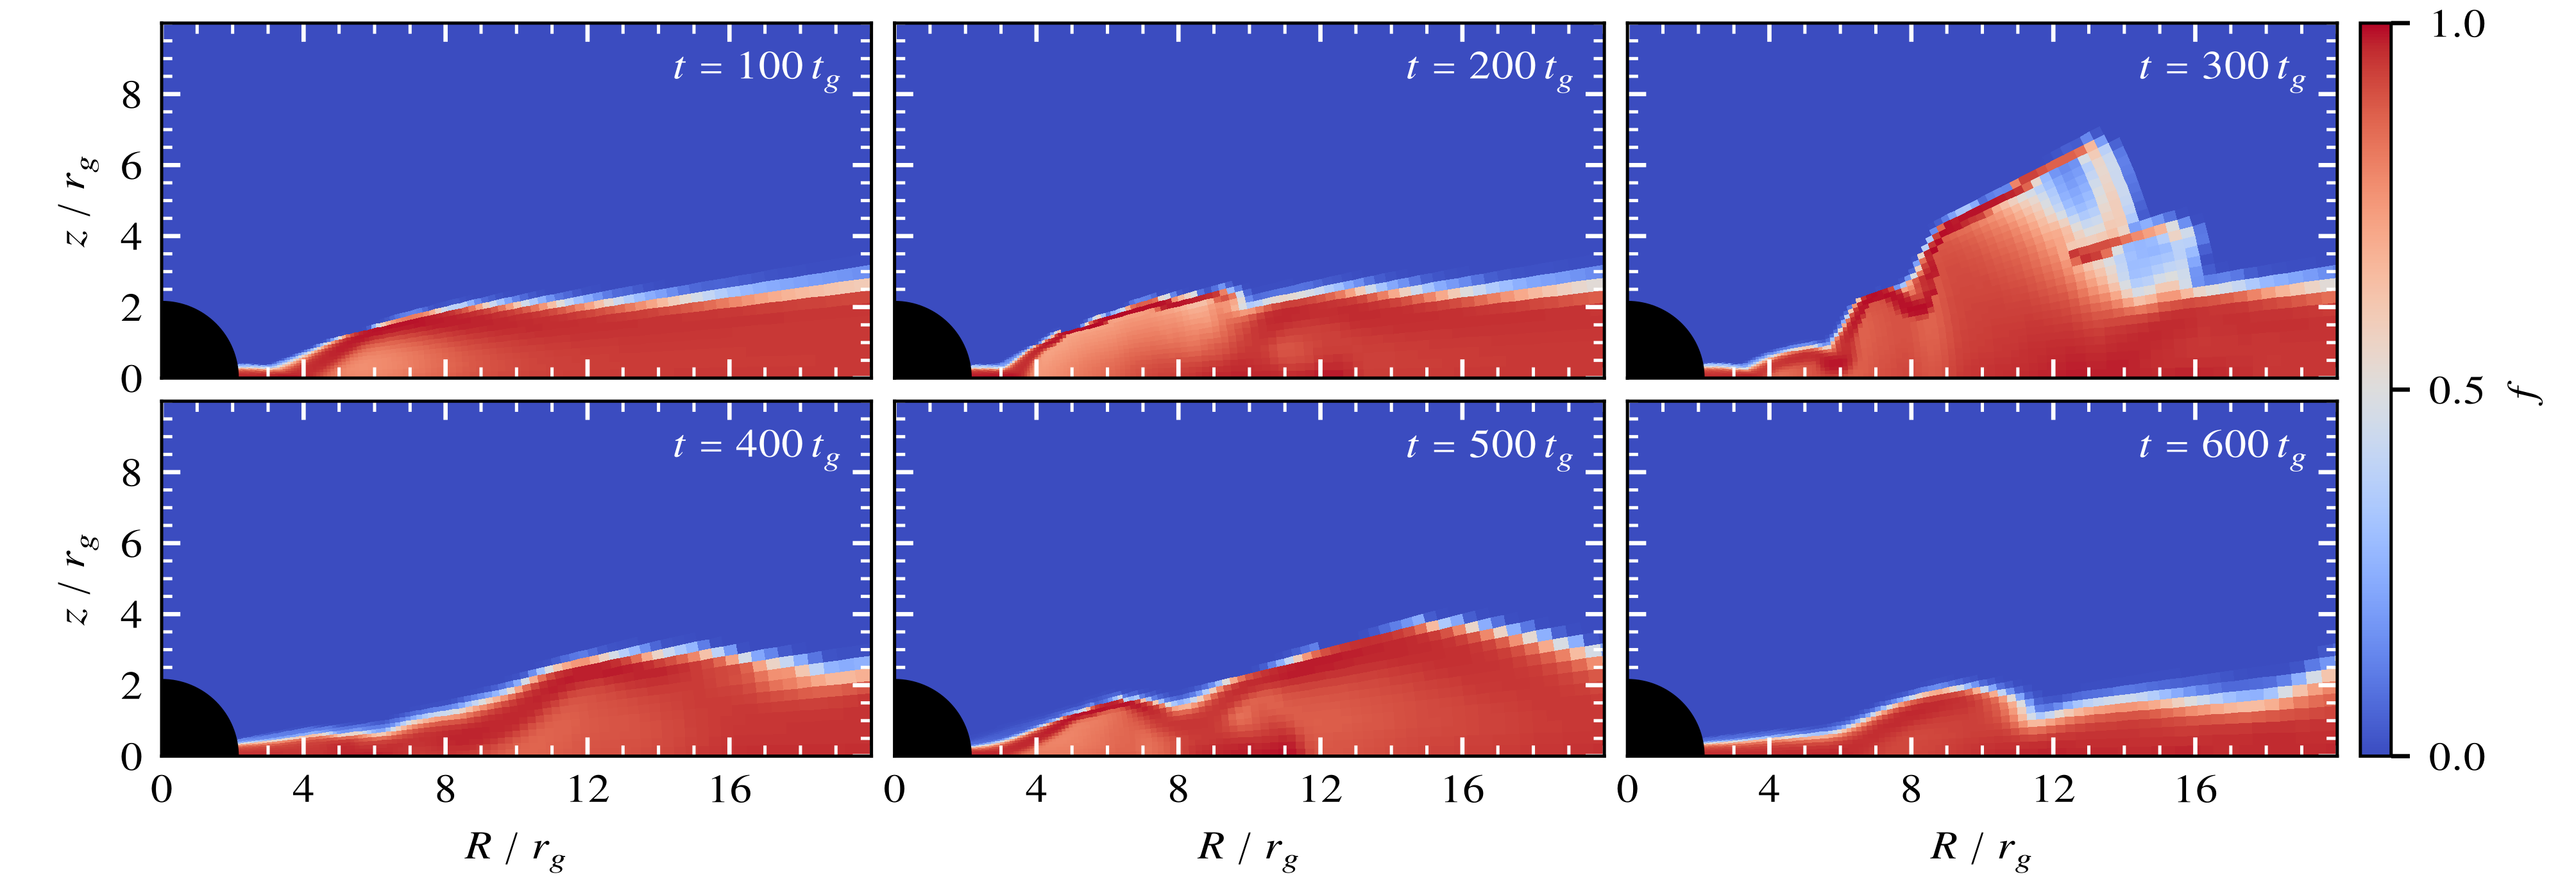
\includegraphics[width=\textwidth, draft=false]{plots/early_f_text.png}
		\caption{\textit{Top:} Rotation velocity of HR, arranged as in \Cref{fig:domain_f_Tg}. \textit{Bottom:} DiskFraction in the
				 early evolution of HR, at the times of \Cref{fig:early}.}
		\label{fig:domain_vphi}
	\end{figure*}

	\begin{figure*}[p]
		\centering
		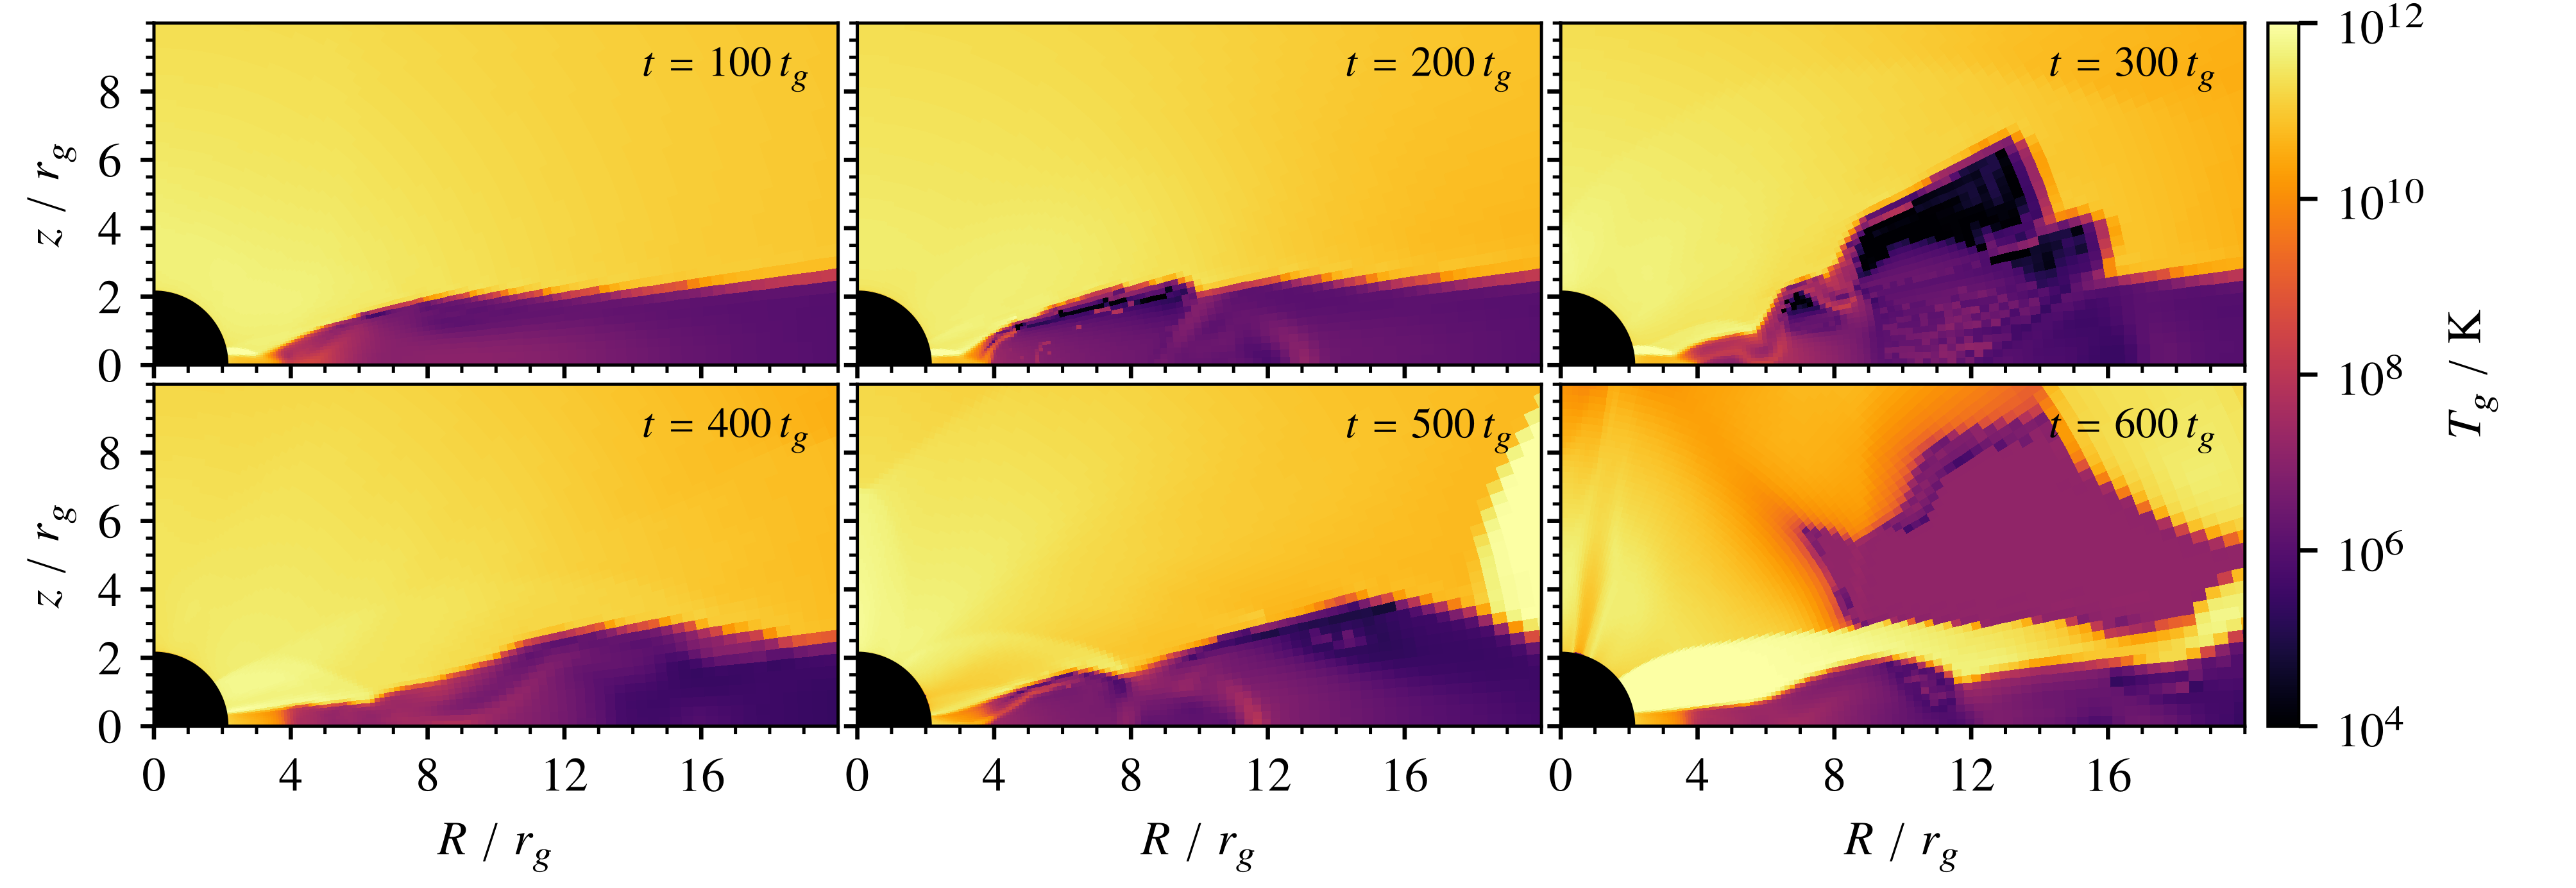
\includegraphics[width=\textwidth, draft=false]{plots/early_Tg_text.png}
		\vspace{0.5\baselineskip}
		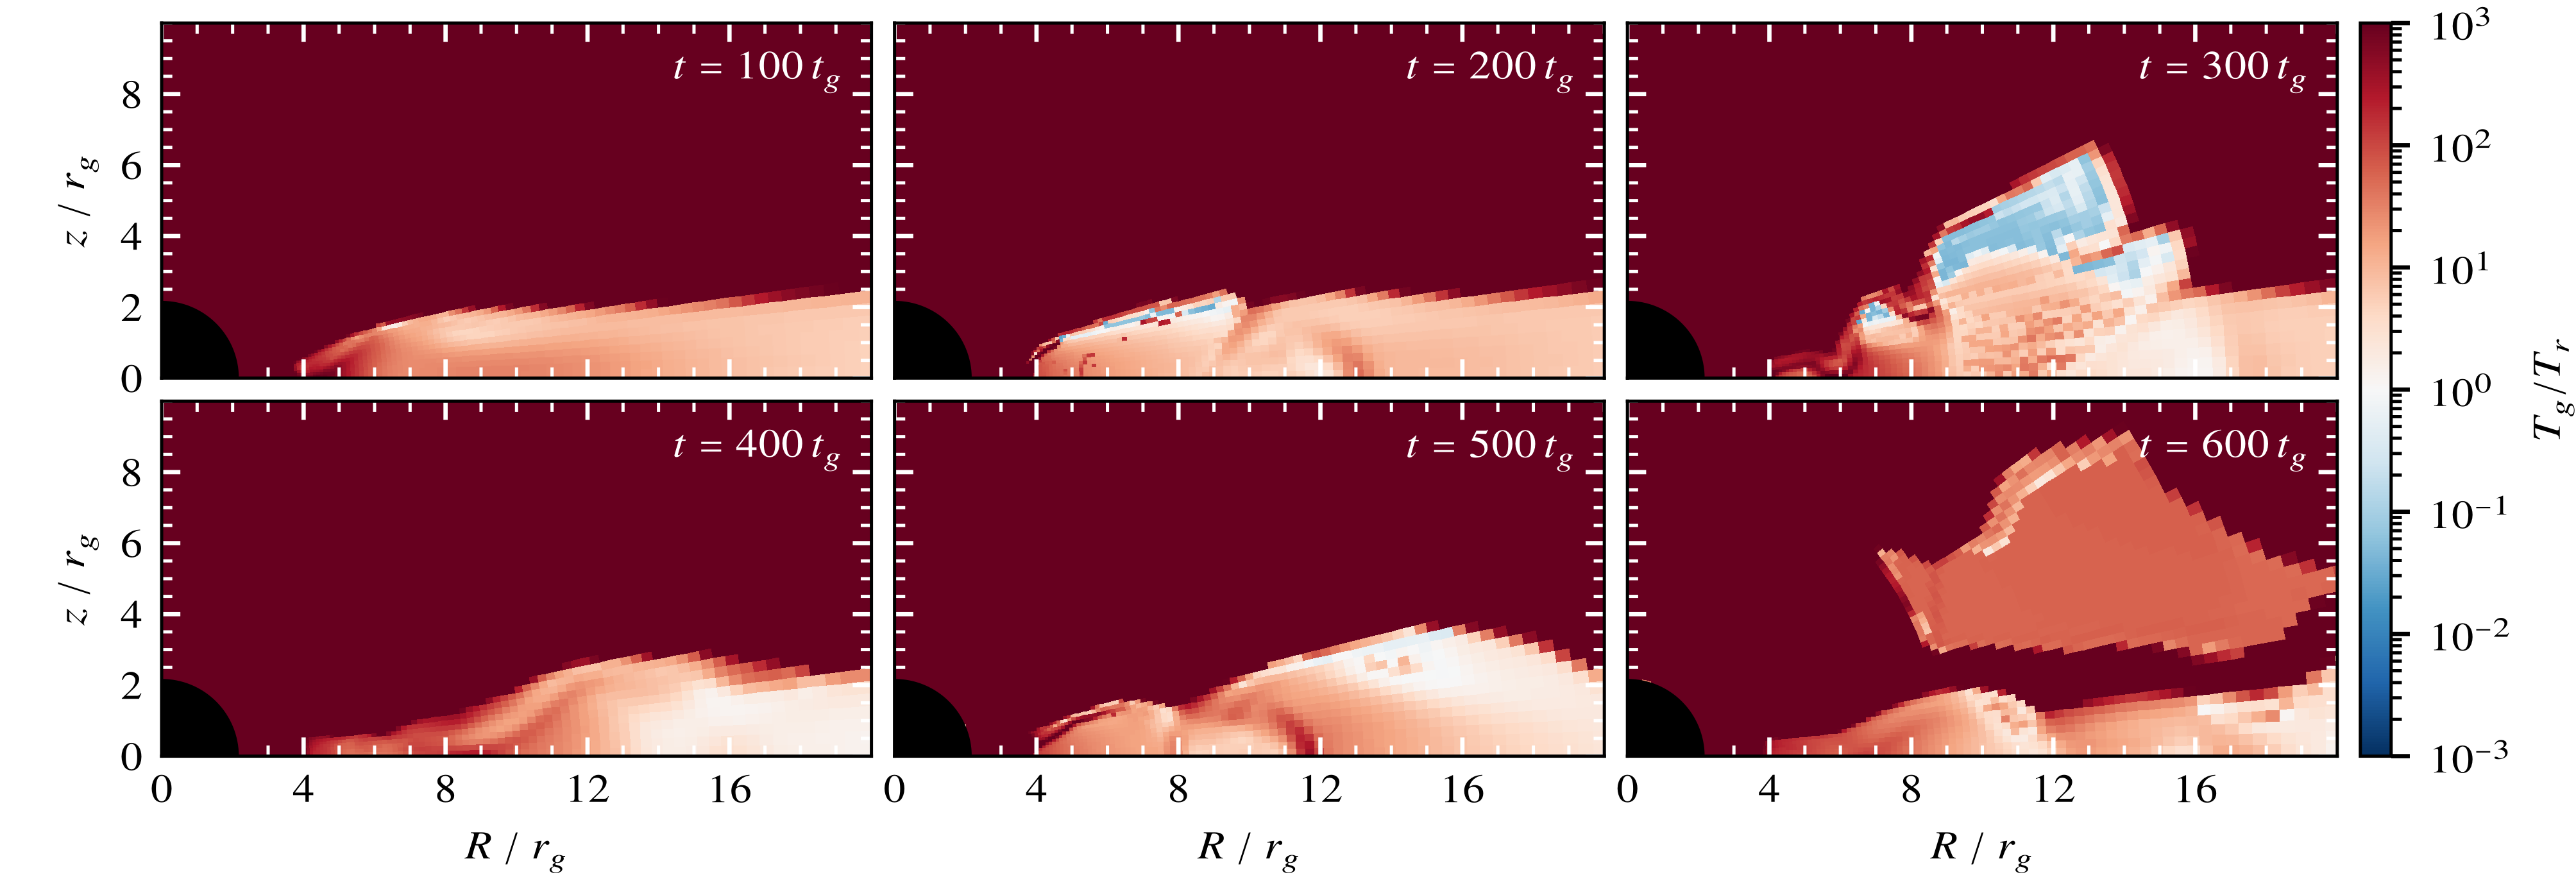
\includegraphics[width=\textwidth, draft=false]{plots/early_ratio_text.png}
		\caption{Gas temperature \textit{(top)} and ratio of gas to radiation temperature \textit{(bottom)} in the early evolution
				 of HR.}
		\label{fig:early_T}
	\end{figure*}

	\begin{figure*}[p]
		\centering
		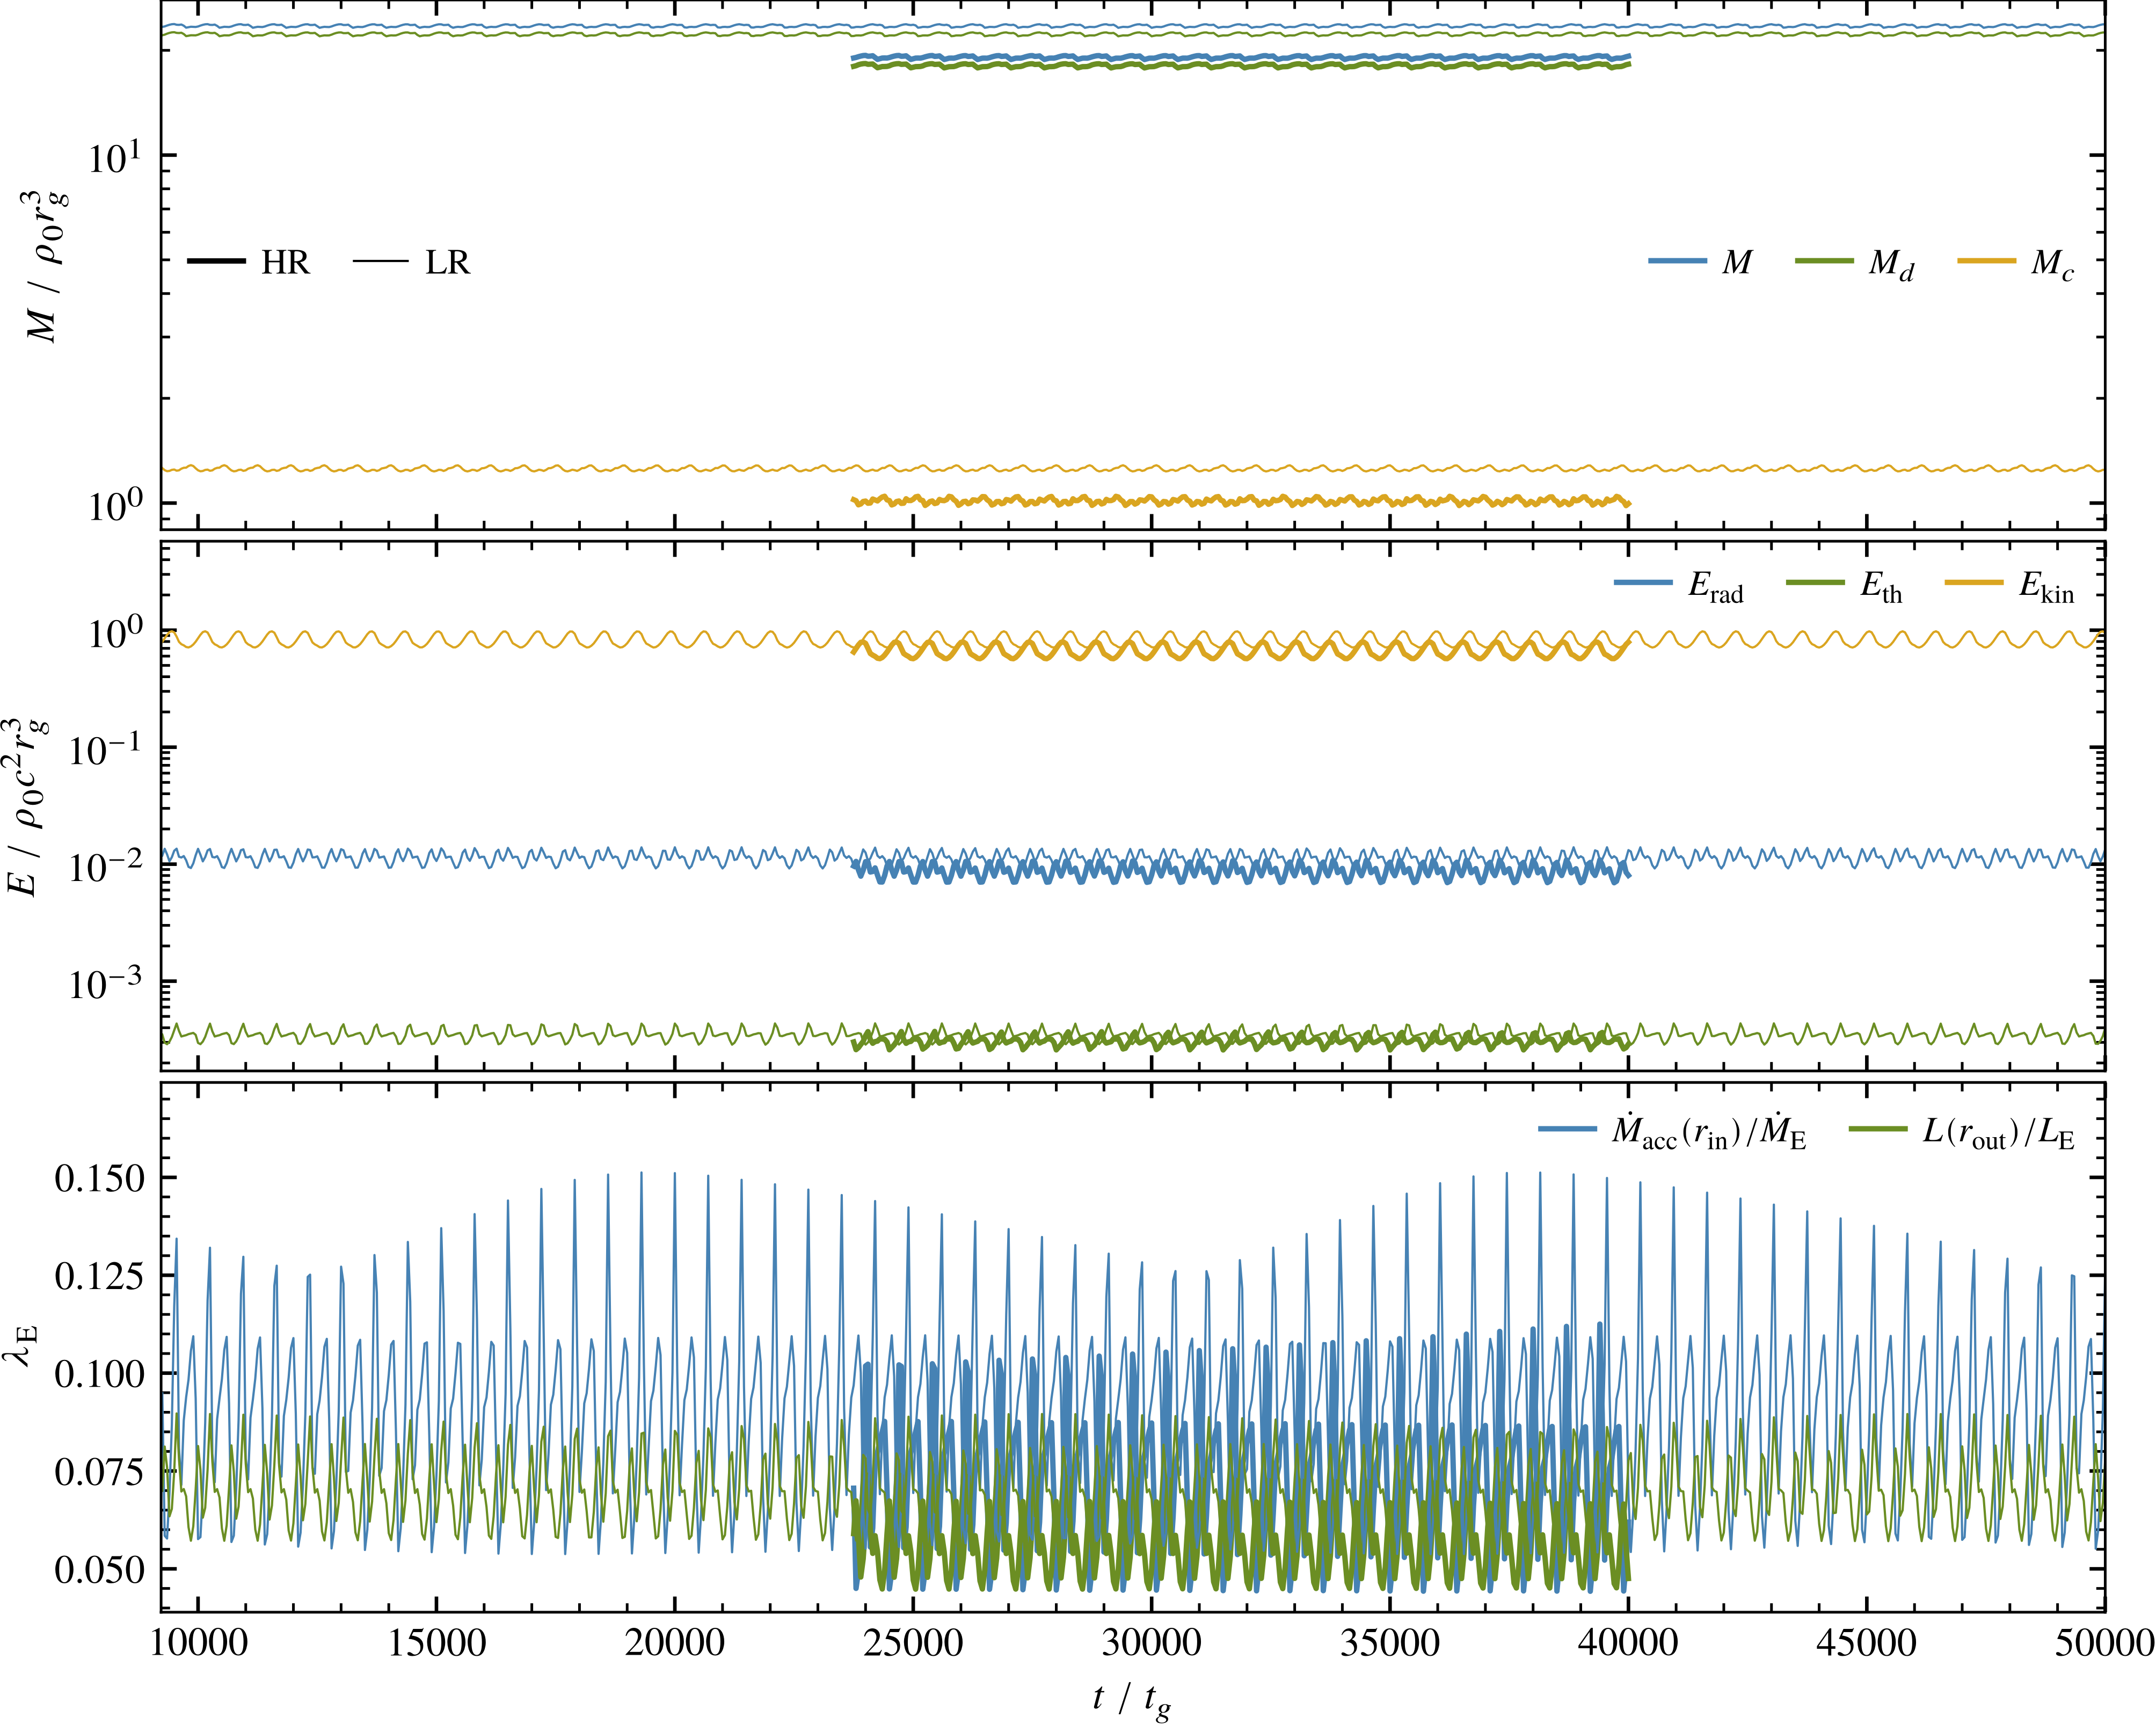
\includegraphics[width=\textwidth, draft=false]{plots/window_text.png}
		\caption{Masses, energies and Eddington ratios of accretion and luminosity of both runs in their steady states.}
		\label{fig:window}
	\end{figure*}

	\begin{figure*}[p]
		\centering
		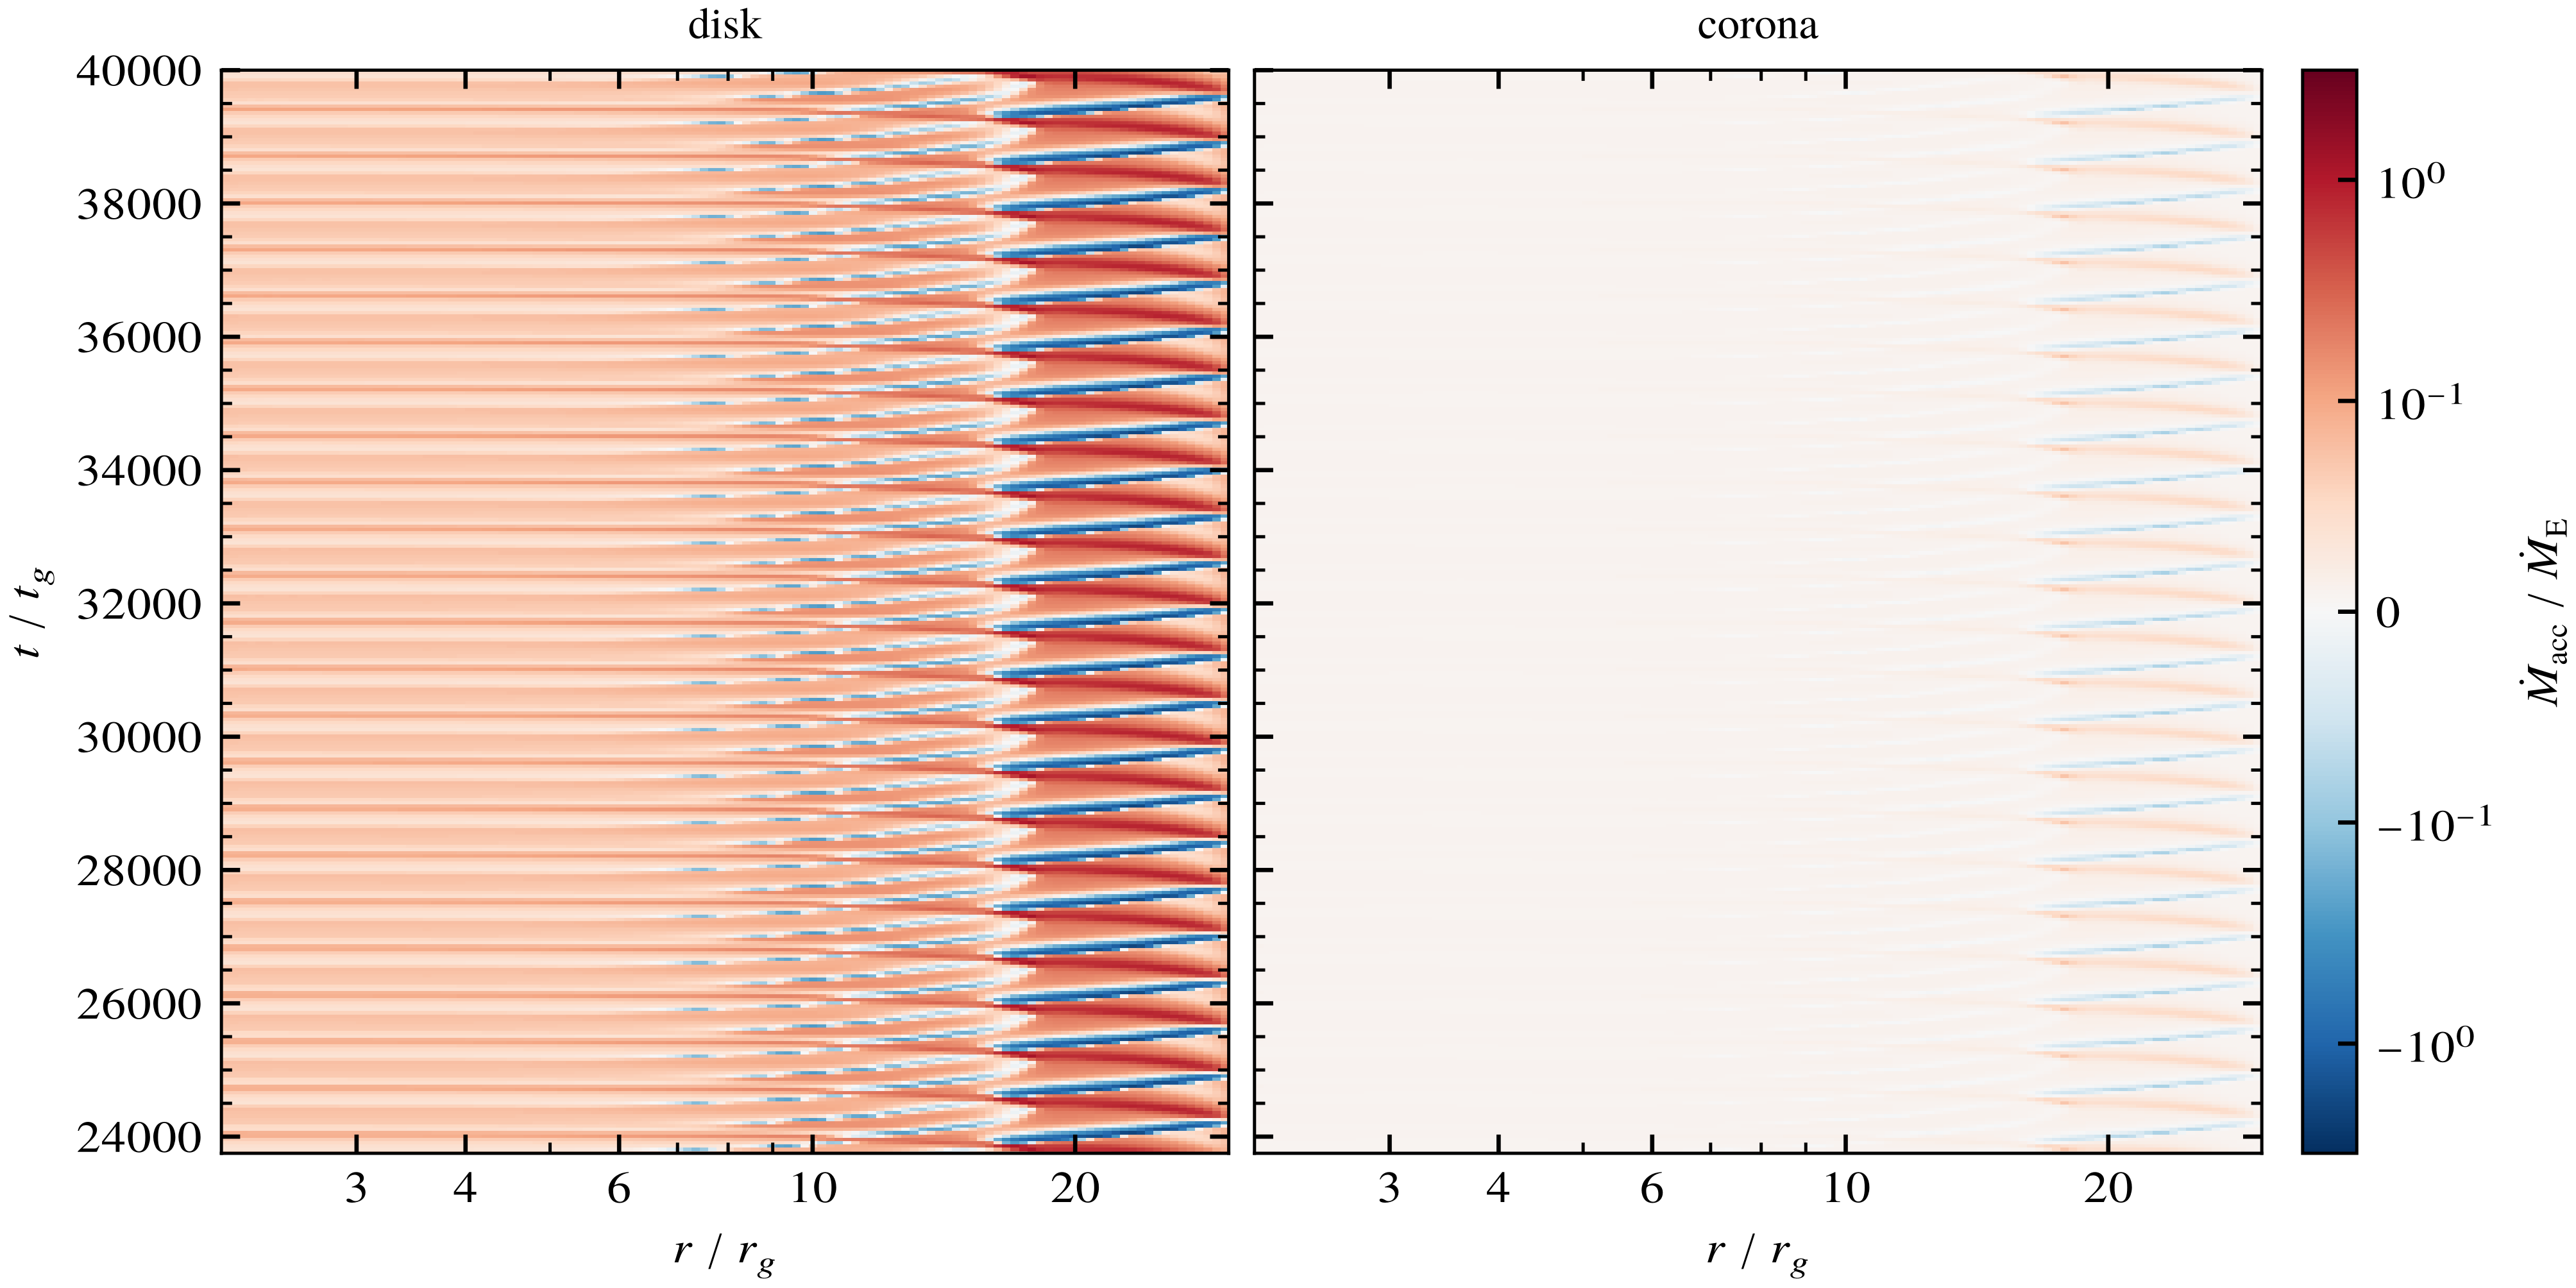
\includegraphics[width=\textwidth, draft=false]{plots/spacetime_mdot_text.png}
		\vspace{0.5\baselineskip}
		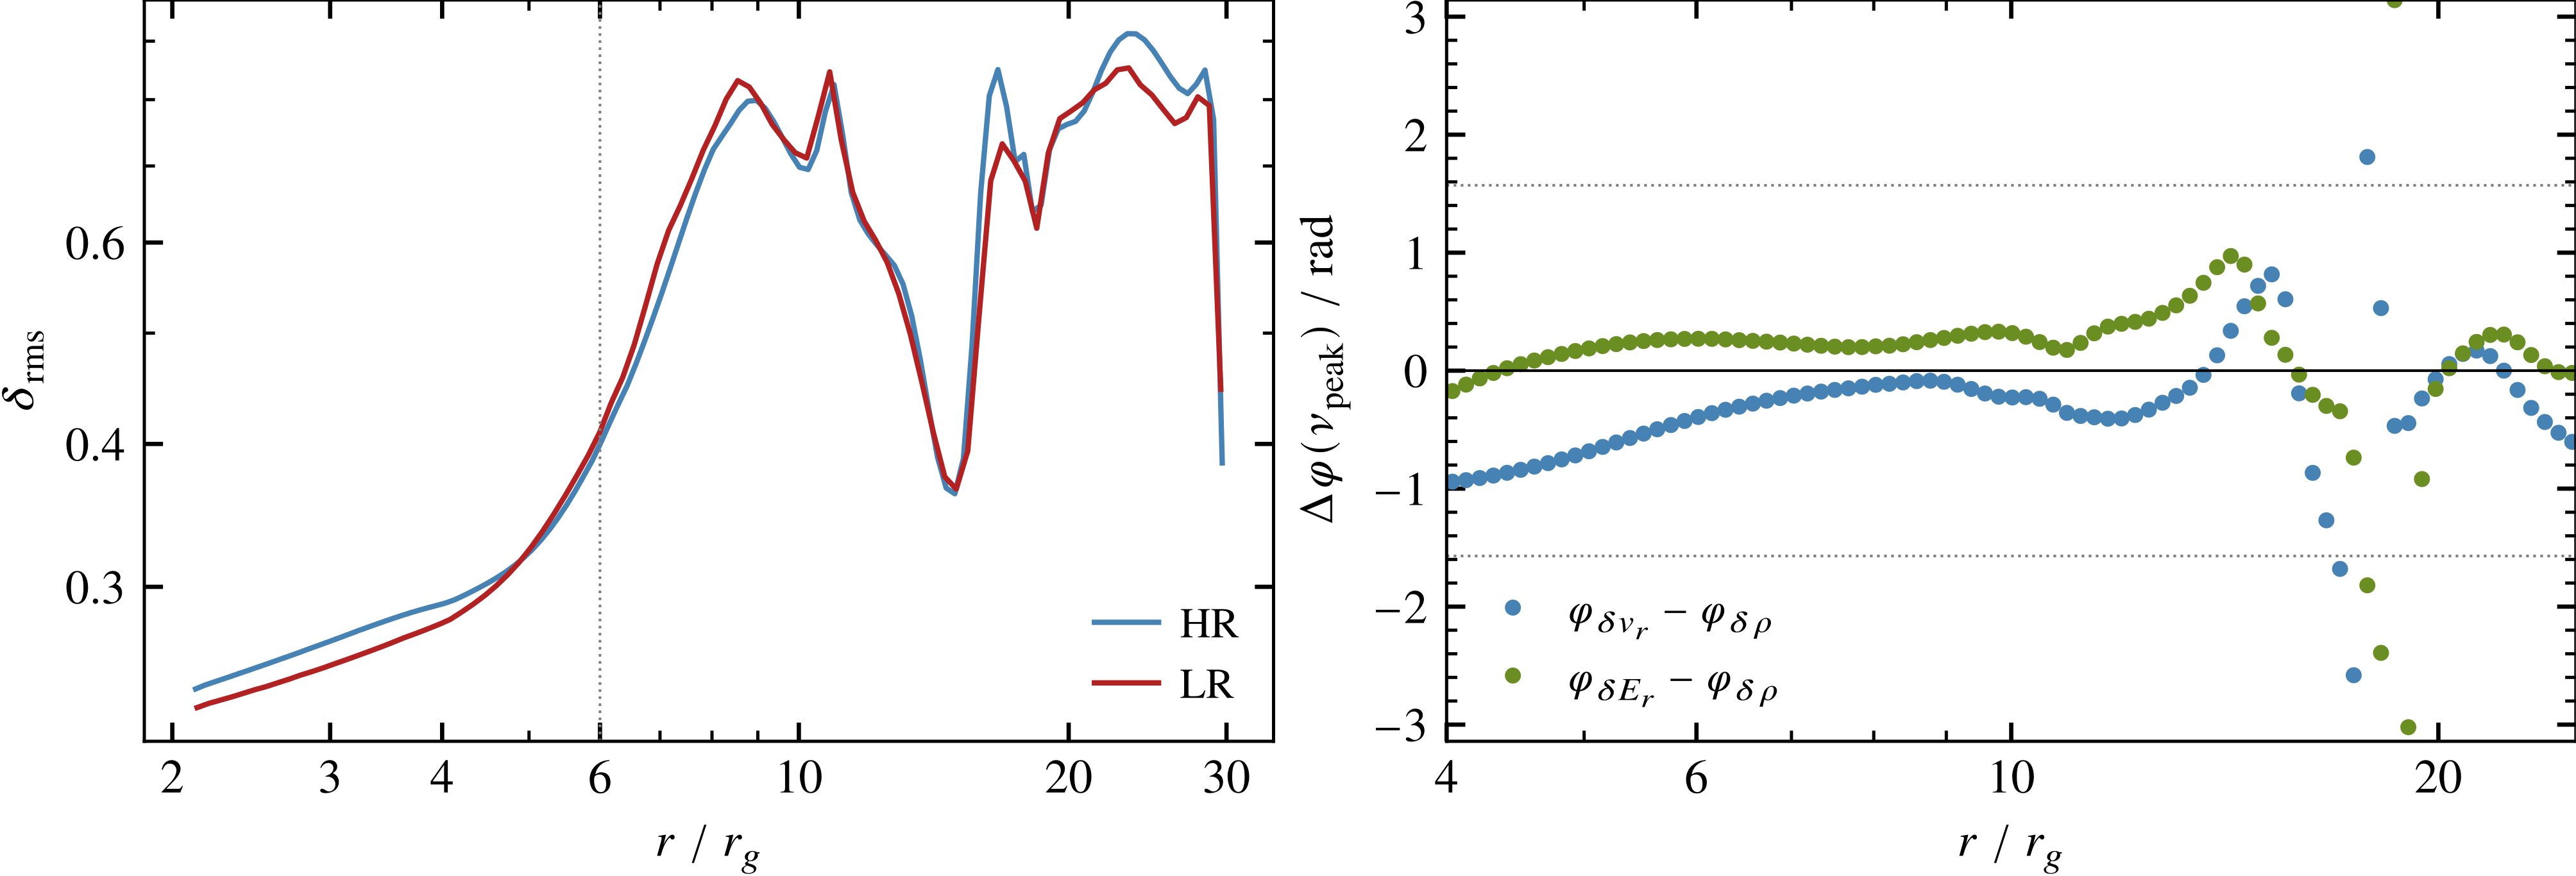
\includegraphics[width=\textwidth, draft=false]{plots/rms_cross_text.png}
		\caption{\textit{Top:} Accretion rate of disk and corona in HR over the steady state. \textit{Bottom:} Root mean square of the
				 surface density perturbation of both runs, and the phase differences of radial velocity and radiation energy relative
				 to density at the peak frequency in HR.}
		\label{fig:spacetime_mdot}
	\end{figure*}

	\begin{figure*}[p]
		\centering
		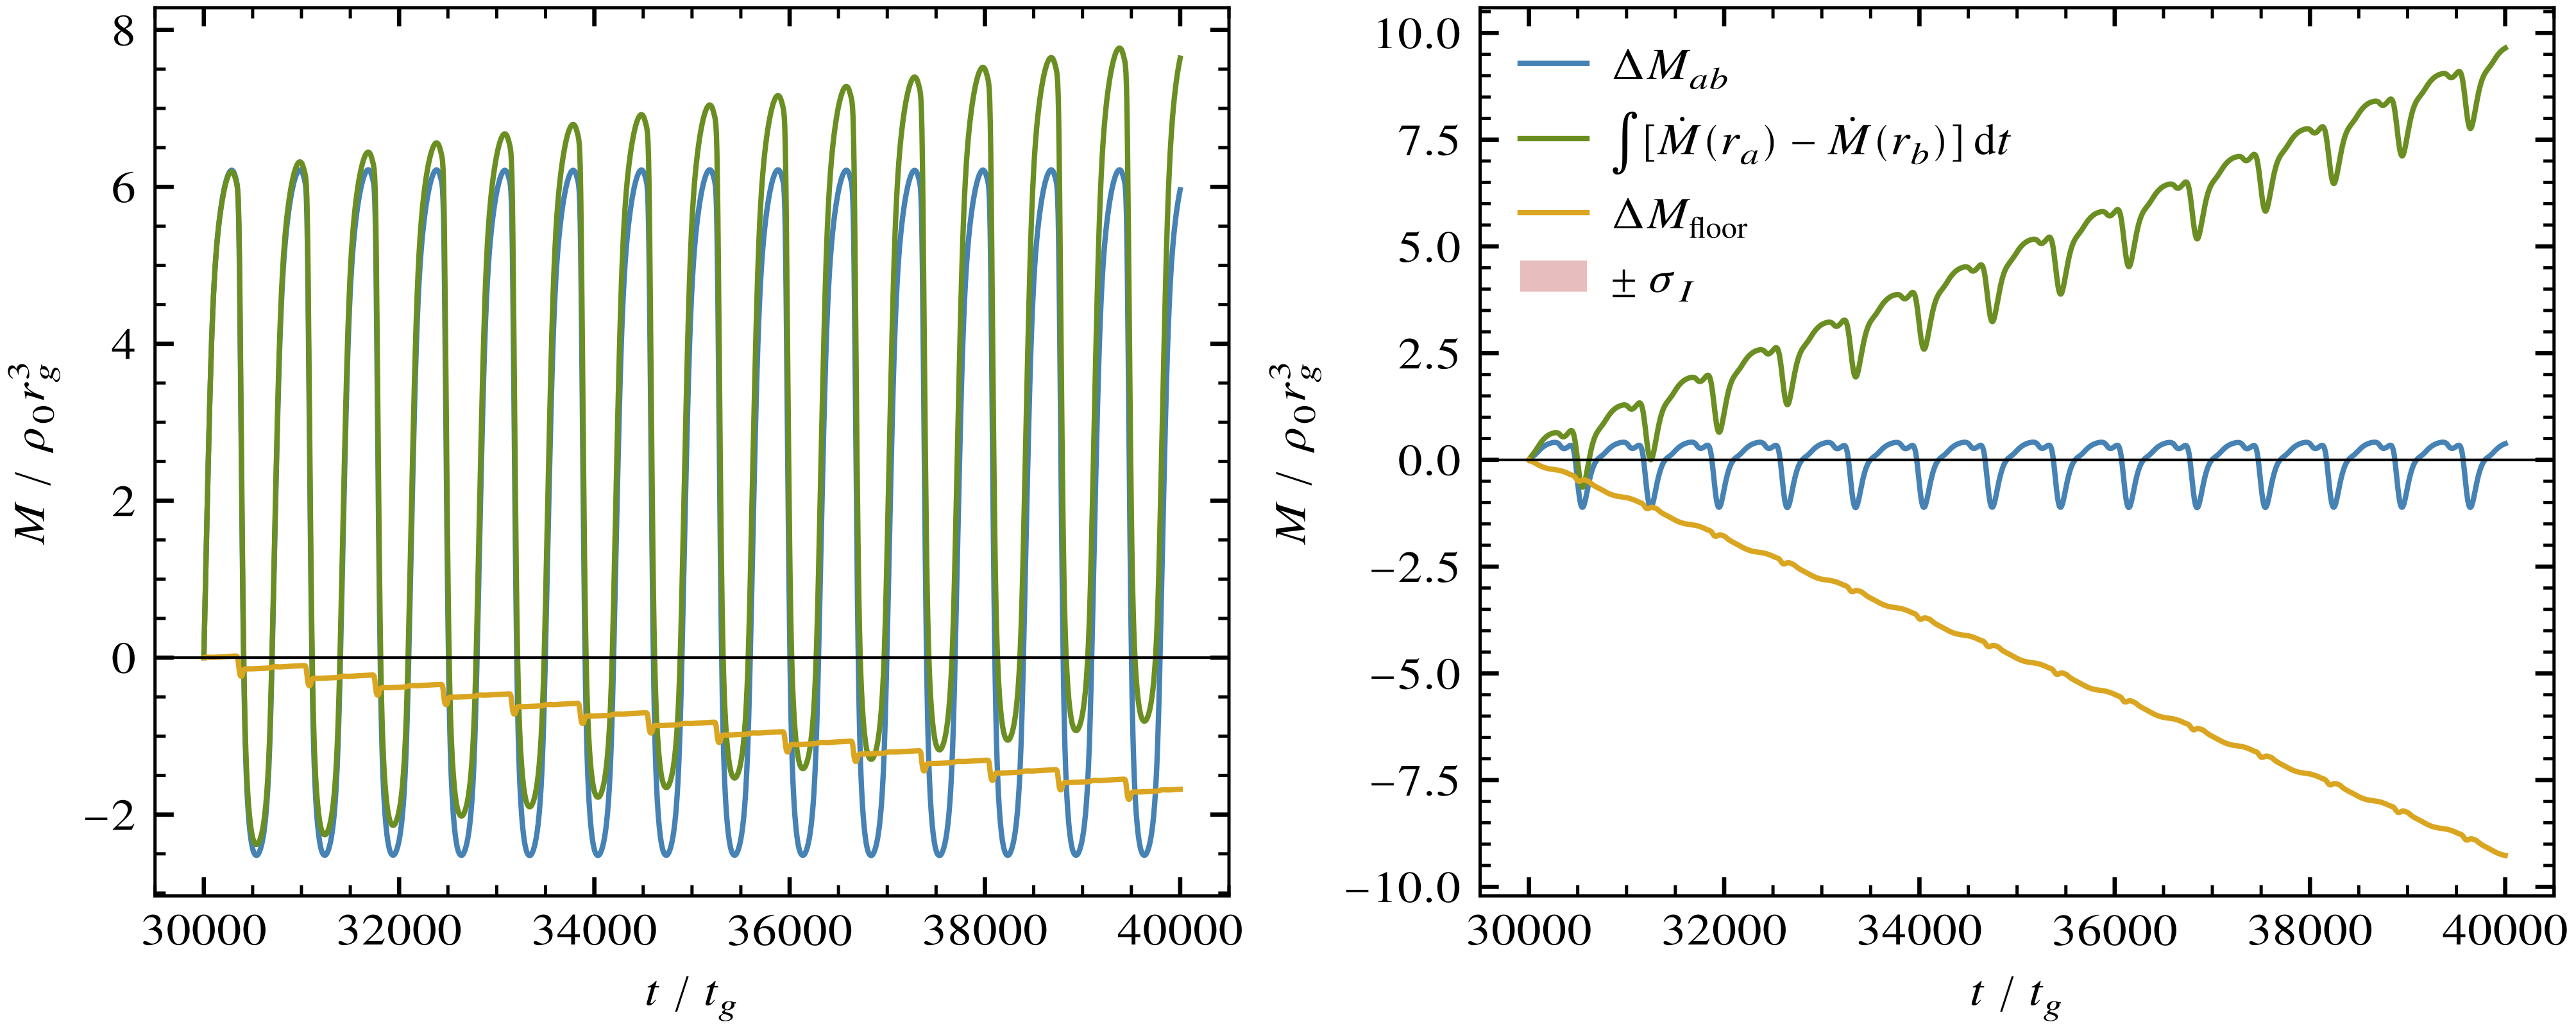
\includegraphics[width=\textwidth, draft=false]{plots/budget_text.png}
		\vspace{0.5\baselineskip}
		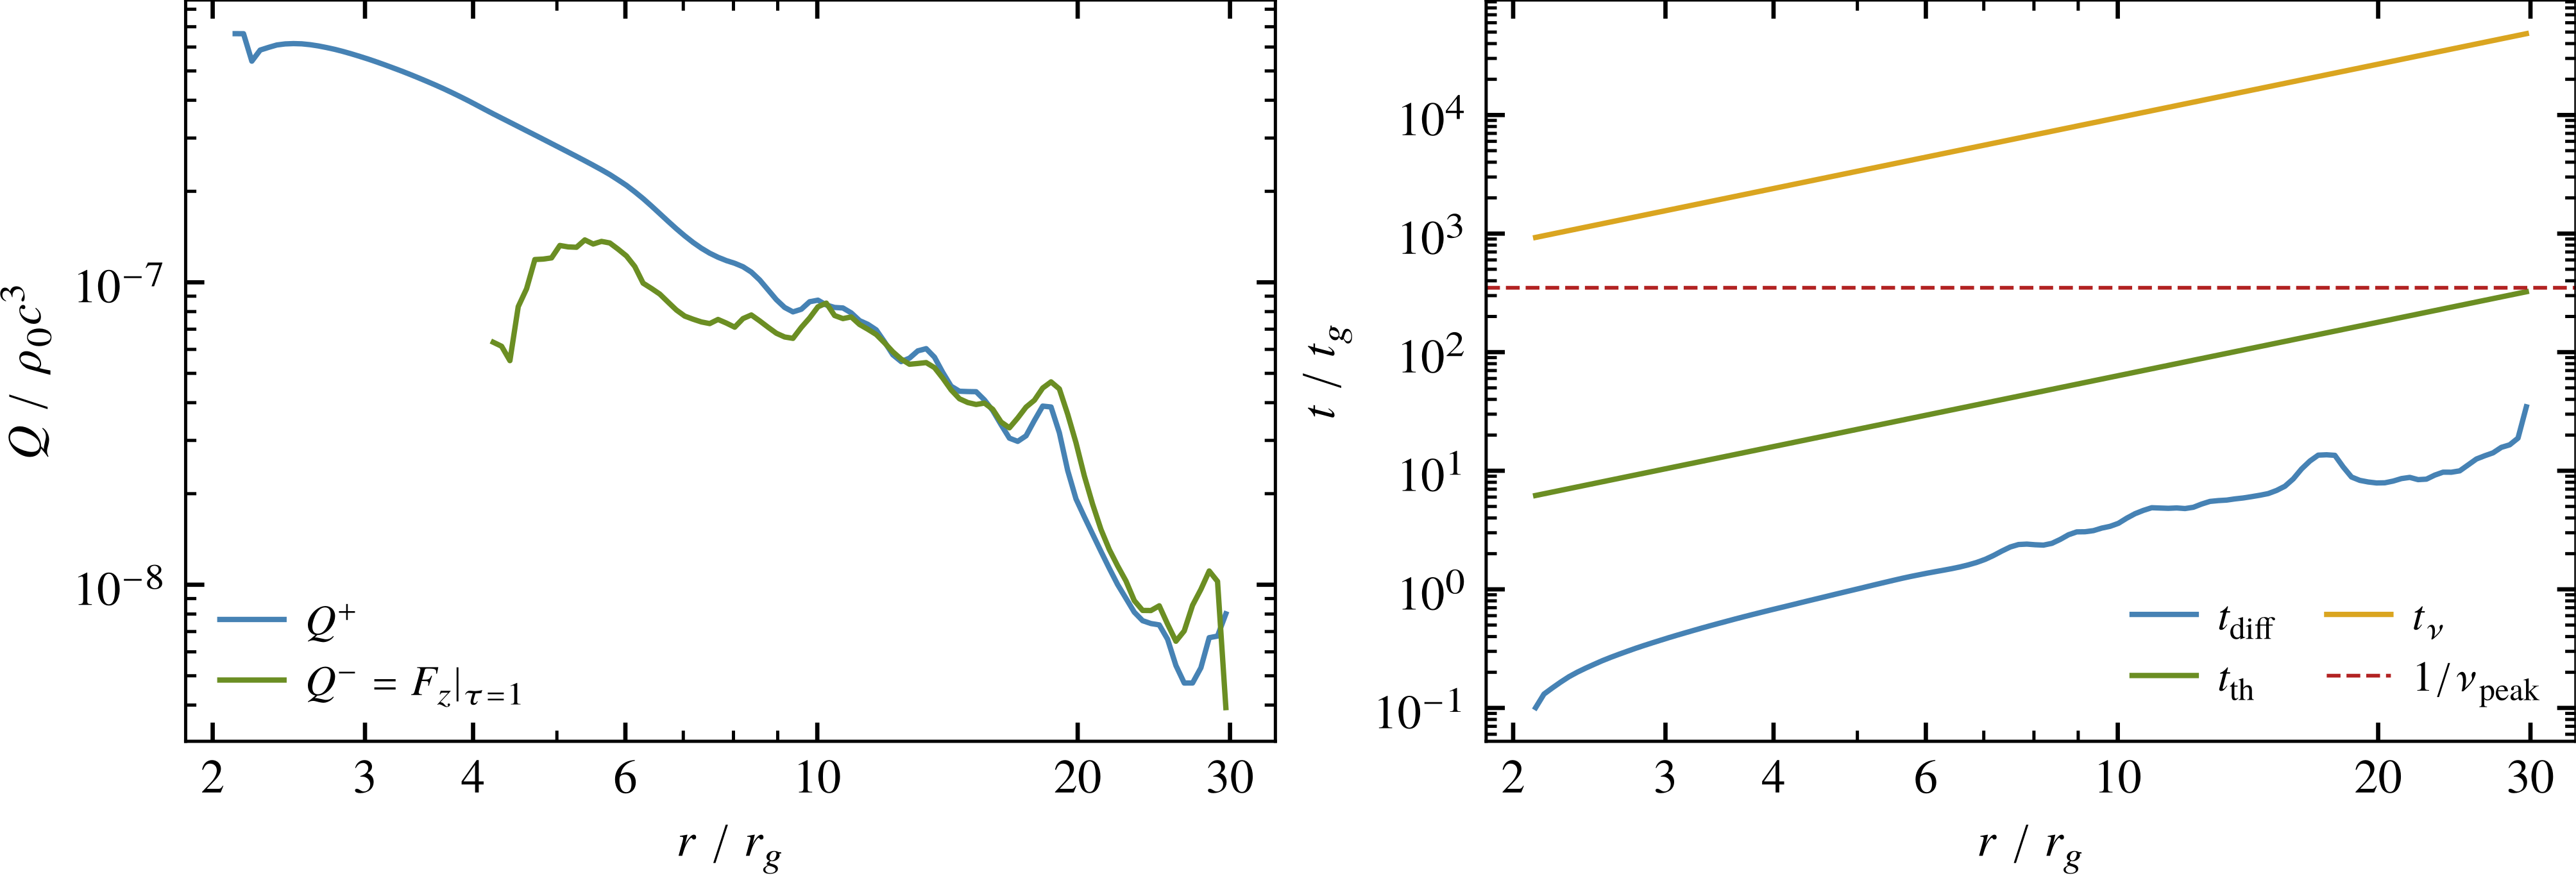
\includegraphics[width=\textwidth, draft=false]{plots/balance_text.png}
		\caption{\textit{Top:} Mass budget of HR between the radii \num{2.5} and \num{25} \textit{(left)} and for the full domain
				 \textit{(right)}. \textit{Bottom:} Vertically integrated heating and the flux at unit optical depth \textit{(left)} as
				 well as diffusion, thermal and viscous times compared with the wave period \textit{(right)}.}
		\label{fig:budget}
	\end{figure*}

	\begin{figure*}[p]
		\centering
		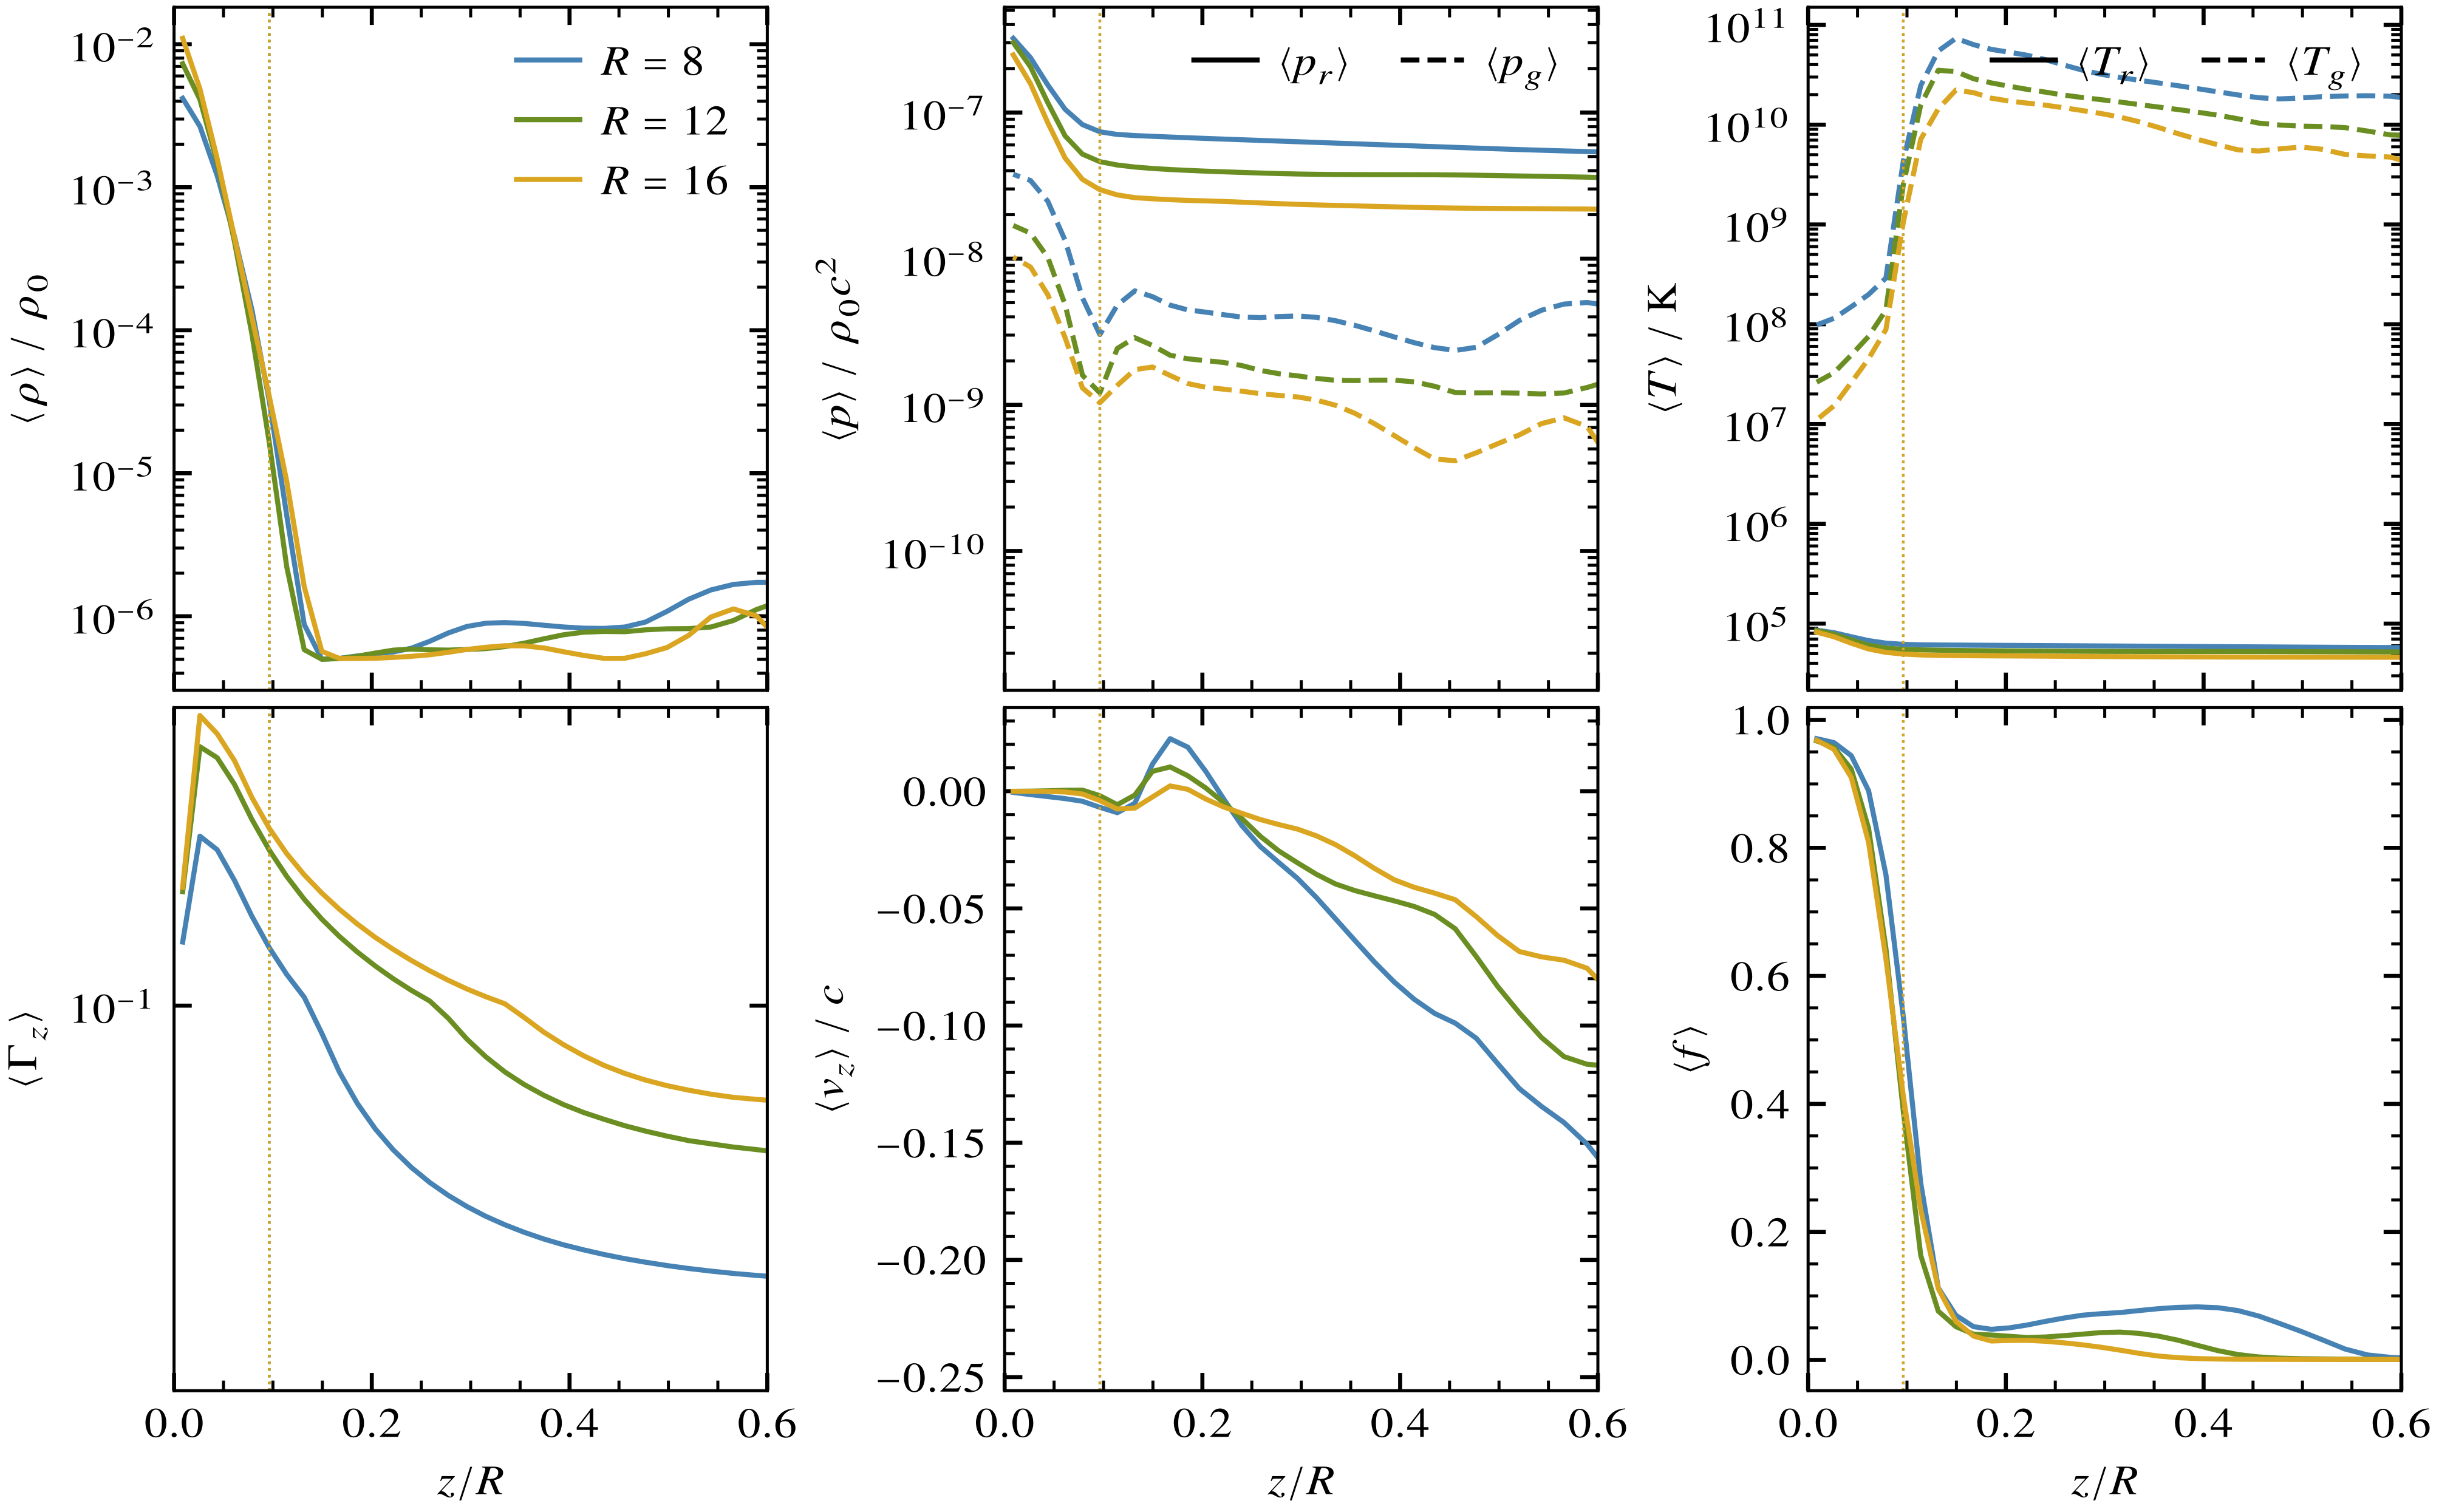
\includegraphics[width=\textwidth, draft=false]{plots/vertical_text.png}
		\caption{Time averaged vertical profiles of HR at three cylindrical radii. Dotted lines mark the disk surface where
				 $f = 0.5$ holds.}
		\label{fig:vertical}
	\end{figure*}

	\begin{figure*}[p]
		\centering
		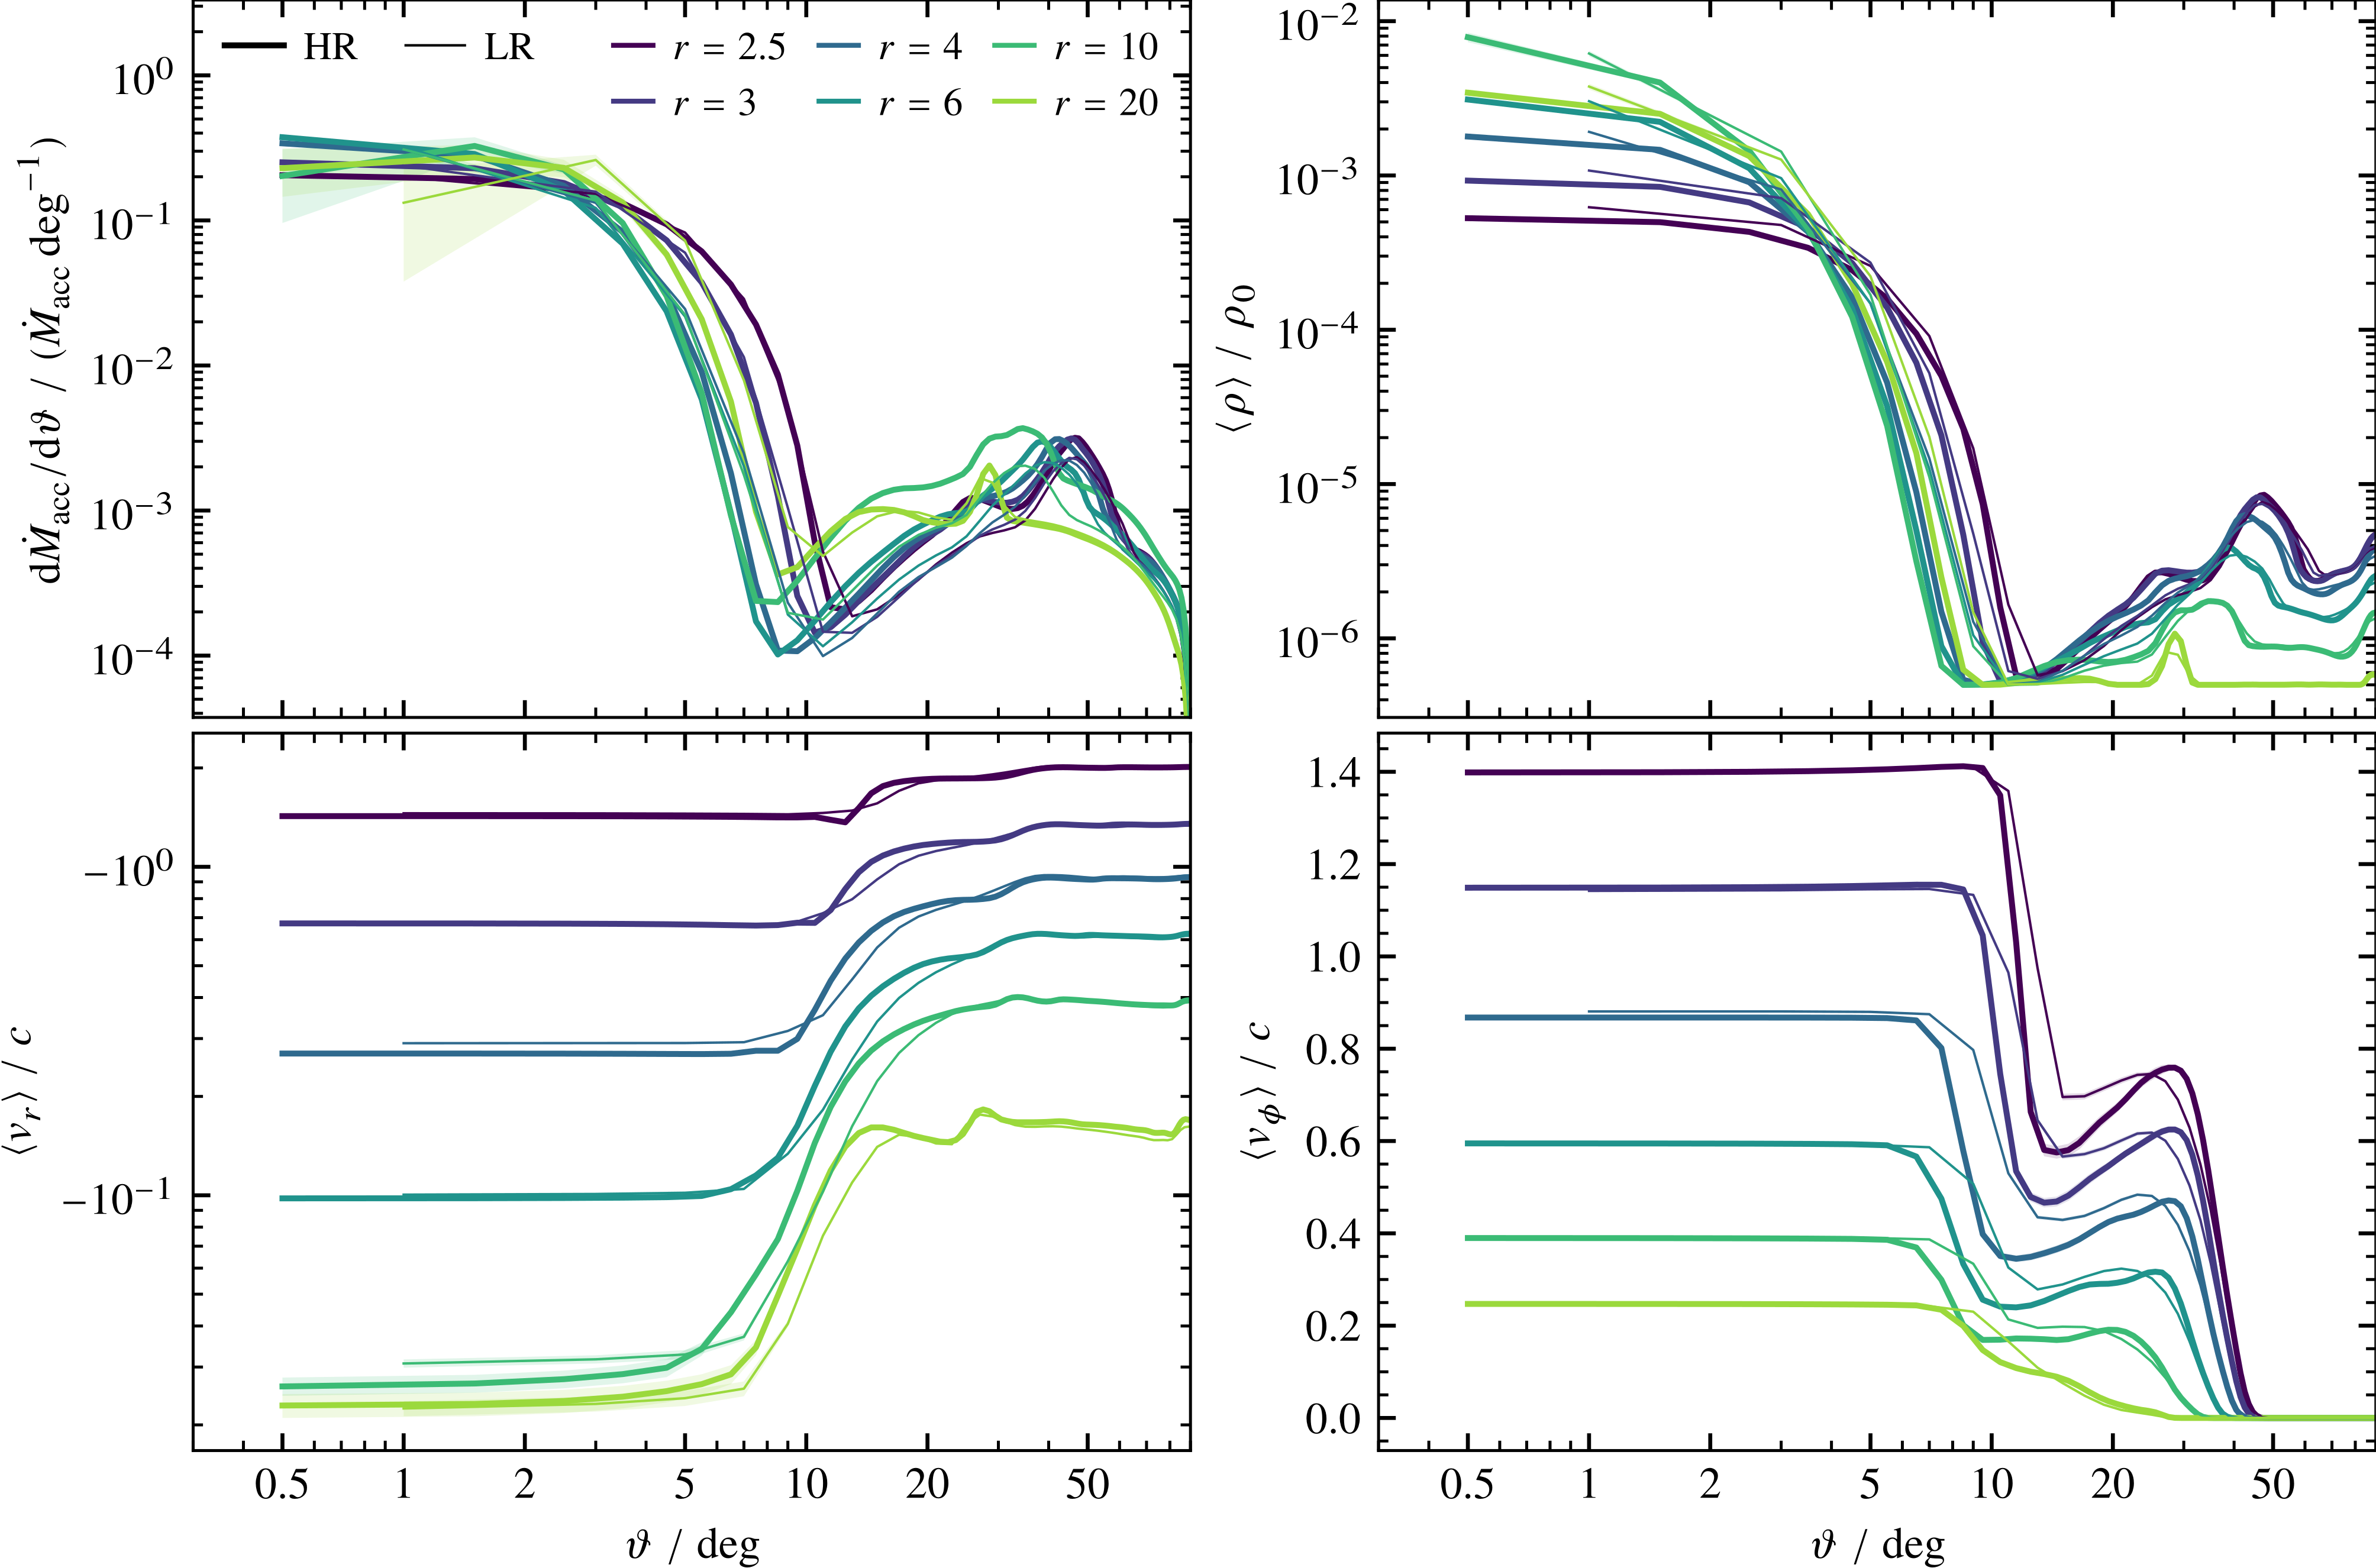
\includegraphics[width=\textwidth, draft=false]{plots/angular_text.png}
		\caption{Time averaged angular profiles of net inflow, density, radial and rotation velocity at several radii for both
				 runs.}
		\label{fig:angular_full}
	\end{figure*}

\end{document}
